\documentclass[]{book}
\usepackage{lmodern}
\usepackage{amssymb,amsmath}
\usepackage{ifxetex,ifluatex}
\usepackage{fixltx2e} % provides \textsubscript
\ifnum 0\ifxetex 1\fi\ifluatex 1\fi=0 % if pdftex
  \usepackage[T1]{fontenc}
  \usepackage[utf8]{inputenc}
\else % if luatex or xelatex
  \ifxetex
    \usepackage{mathspec}
  \else
    \usepackage{fontspec}
  \fi
  \defaultfontfeatures{Ligatures=TeX,Scale=MatchLowercase}
\fi
% use upquote if available, for straight quotes in verbatim environments
\IfFileExists{upquote.sty}{\usepackage{upquote}}{}
% use microtype if available
\IfFileExists{microtype.sty}{%
\usepackage{microtype}
\UseMicrotypeSet[protrusion]{basicmath} % disable protrusion for tt fonts
}{}
\usepackage[margin=2cm]{geometry}
\usepackage{hyperref}
\hypersetup{unicode=true,
            pdftitle={Note di R},
            pdfauthor={Federico Reali},
            pdfborder={0 0 0},
            breaklinks=true}
\urlstyle{same}  % don't use monospace font for urls
\usepackage{natbib}
\bibliographystyle{apalike}
\usepackage{color}
\usepackage{fancyvrb}
\newcommand{\VerbBar}{|}
\newcommand{\VERB}{\Verb[commandchars=\\\{\}]}
\DefineVerbatimEnvironment{Highlighting}{Verbatim}{commandchars=\\\{\}}
% Add ',fontsize=\small' for more characters per line
\usepackage{framed}
\definecolor{shadecolor}{RGB}{248,248,248}
\newenvironment{Shaded}{\begin{snugshade}}{\end{snugshade}}
\newcommand{\AlertTok}[1]{\textcolor[rgb]{0.94,0.16,0.16}{#1}}
\newcommand{\AnnotationTok}[1]{\textcolor[rgb]{0.56,0.35,0.01}{\textbf{\textit{#1}}}}
\newcommand{\AttributeTok}[1]{\textcolor[rgb]{0.77,0.63,0.00}{#1}}
\newcommand{\BaseNTok}[1]{\textcolor[rgb]{0.00,0.00,0.81}{#1}}
\newcommand{\BuiltInTok}[1]{#1}
\newcommand{\CharTok}[1]{\textcolor[rgb]{0.31,0.60,0.02}{#1}}
\newcommand{\CommentTok}[1]{\textcolor[rgb]{0.56,0.35,0.01}{\textit{#1}}}
\newcommand{\CommentVarTok}[1]{\textcolor[rgb]{0.56,0.35,0.01}{\textbf{\textit{#1}}}}
\newcommand{\ConstantTok}[1]{\textcolor[rgb]{0.00,0.00,0.00}{#1}}
\newcommand{\ControlFlowTok}[1]{\textcolor[rgb]{0.13,0.29,0.53}{\textbf{#1}}}
\newcommand{\DataTypeTok}[1]{\textcolor[rgb]{0.13,0.29,0.53}{#1}}
\newcommand{\DecValTok}[1]{\textcolor[rgb]{0.00,0.00,0.81}{#1}}
\newcommand{\DocumentationTok}[1]{\textcolor[rgb]{0.56,0.35,0.01}{\textbf{\textit{#1}}}}
\newcommand{\ErrorTok}[1]{\textcolor[rgb]{0.64,0.00,0.00}{\textbf{#1}}}
\newcommand{\ExtensionTok}[1]{#1}
\newcommand{\FloatTok}[1]{\textcolor[rgb]{0.00,0.00,0.81}{#1}}
\newcommand{\FunctionTok}[1]{\textcolor[rgb]{0.00,0.00,0.00}{#1}}
\newcommand{\ImportTok}[1]{#1}
\newcommand{\InformationTok}[1]{\textcolor[rgb]{0.56,0.35,0.01}{\textbf{\textit{#1}}}}
\newcommand{\KeywordTok}[1]{\textcolor[rgb]{0.13,0.29,0.53}{\textbf{#1}}}
\newcommand{\NormalTok}[1]{#1}
\newcommand{\OperatorTok}[1]{\textcolor[rgb]{0.81,0.36,0.00}{\textbf{#1}}}
\newcommand{\OtherTok}[1]{\textcolor[rgb]{0.56,0.35,0.01}{#1}}
\newcommand{\PreprocessorTok}[1]{\textcolor[rgb]{0.56,0.35,0.01}{\textit{#1}}}
\newcommand{\RegionMarkerTok}[1]{#1}
\newcommand{\SpecialCharTok}[1]{\textcolor[rgb]{0.00,0.00,0.00}{#1}}
\newcommand{\SpecialStringTok}[1]{\textcolor[rgb]{0.31,0.60,0.02}{#1}}
\newcommand{\StringTok}[1]{\textcolor[rgb]{0.31,0.60,0.02}{#1}}
\newcommand{\VariableTok}[1]{\textcolor[rgb]{0.00,0.00,0.00}{#1}}
\newcommand{\VerbatimStringTok}[1]{\textcolor[rgb]{0.31,0.60,0.02}{#1}}
\newcommand{\WarningTok}[1]{\textcolor[rgb]{0.56,0.35,0.01}{\textbf{\textit{#1}}}}
\usepackage{longtable,booktabs}
\usepackage{graphicx,grffile}
\makeatletter
\def\maxwidth{\ifdim\Gin@nat@width>\linewidth\linewidth\else\Gin@nat@width\fi}
\def\maxheight{\ifdim\Gin@nat@height>\textheight\textheight\else\Gin@nat@height\fi}
\makeatother
% Scale images if necessary, so that they will not overflow the page
% margins by default, and it is still possible to overwrite the defaults
% using explicit options in \includegraphics[width, height, ...]{}
\setkeys{Gin}{width=\maxwidth,height=\maxheight,keepaspectratio}
\IfFileExists{parskip.sty}{%
\usepackage{parskip}
}{% else
\setlength{\parindent}{0pt}
\setlength{\parskip}{6pt plus 2pt minus 1pt}
}
\setlength{\emergencystretch}{3em}  % prevent overfull lines
\providecommand{\tightlist}{%
  \setlength{\itemsep}{0pt}\setlength{\parskip}{0pt}}
\setcounter{secnumdepth}{5}
% Redefines (sub)paragraphs to behave more like sections
\ifx\paragraph\undefined\else
\let\oldparagraph\paragraph
\renewcommand{\paragraph}[1]{\oldparagraph{#1}\mbox{}}
\fi
\ifx\subparagraph\undefined\else
\let\oldsubparagraph\subparagraph
\renewcommand{\subparagraph}[1]{\oldsubparagraph{#1}\mbox{}}
\fi

%%% Use protect on footnotes to avoid problems with footnotes in titles
\let\rmarkdownfootnote\footnote%
\def\footnote{\protect\rmarkdownfootnote}

%%% Change title format to be more compact
\usepackage{titling}

% Create subtitle command for use in maketitle
\providecommand{\subtitle}[1]{
  \posttitle{
    \begin{center}\large#1\end{center}
    }
}

\setlength{\droptitle}{-2em}

  \title{Note di R}
    \pretitle{\vspace{\droptitle}\centering\huge}
  \posttitle{\par}
    \author{Federico Reali}
    \preauthor{\centering\large\emph}
  \postauthor{\par}
      \predate{\centering\large\emph}
  \postdate{\par}
    \date{06/06/2019}

\usepackage{booktabs}
\usepackage{amsthm}
\makeatletter
\def\thm@space@setup{%
  \thm@preskip=8pt plus 2pt minus 4pt
  \thm@postskip=\thm@preskip
}
\makeatother

\begin{document}
\maketitle

{
\setcounter{tocdepth}{1}
\tableofcontents
}
\hypertarget{premessa}{%
\chapter*{Premessa}\label{premessa}}
\addcontentsline{toc}{chapter}{Premessa}

Questo libro racchiude le note riguardanti il laboratorio di R del corso di Probabilità e Statistica Matematica dell'anno accademico 2018/2019.

Il materiale contenuto si intende ad uso degli studenti. Può contenere errori, typos ed imprecisioni.

Questo e-book è stato ottenuto grazie usando il pacchetto \textbf{bookdown} \citep{R-bookdown} e la guida \citep{xie2015}.

\hypertarget{primi-passi-con-r}{%
\chapter{Primi passi con R}\label{primi-passi-con-r}}


\includegraphics{./media/Rlogo.png}

In questa prima parte vedremo quali sono i passi base per istallare R e Rstudio sul nostro computer.

\hypertarget{perche-r}{%
\section{Perché R}\label{perche-r}}

\begin{quote}
R is a free software environment for statistical computing and graphics.
It compiles and runs on a wide variety of UNIX platforms, Windows and MacOS.

 The R Foundation
\end{quote}

R è un versatile linguaggio di programmazione che sta particolarmente a cuore alla comunità che si occupa di statistica, per questo esistono molte pagine volte ad insegnarne l'uso, così come molti blog e forum dove gli utenti possono cercare risposte alle loro domande realtive all'uso.

R è un software libero disponibile per le maggiori piattaforme, inclusi Windows, Mac e diverse distribuzioni di Linux.

Per esempio, possiamo trovare molte guide su come installare R sul nostro computer Windows, Mac o Linux. Una semplice ricerca su google produce innumerevoli guide e tutorial su come farlo.


\includegraphics{./media/Google_Install_R.png}

Noi seguiremo una via molto diretta che segue due passi fondamentali:

\begin{itemize}
\tightlist
\item
  l'istallazione di R vera e propria;
\item
  l'istallazione di un interfaccia.
\end{itemize}

Installeremo la {[}versione{]} (\url{https://www.r-project.org/}) di R rilasciata l'11/03/2019 e tra le innumerevoli interfacce per R, noi useremo \href{https://www.rstudio.com/products/rstudio/}{R Studio}. Si noti che tra pochi giorni sarà disponibile la versione 3.6.0.

\begin{figure}
\centering
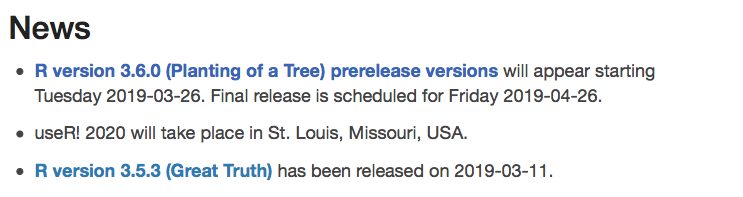
\includegraphics{./media/R_release_2019.png}
\caption{Release di R}
\end{figure}

\hypertarget{installare-r}{%
\section{Installare R}\label{installare-r}}

Procediamo con l'istallazione di R

\hypertarget{scaricare-r}{%
\subsection{Scaricare R}\label{scaricare-r}}

Le varie release di R sono disponibili attraverso il sito \href{https://cran.r-project.org/}{cran}, dove è possibilie selezionare il server più vicino da cui fare il download dei file di istallazione.

Ad esempio possiamo scegliere il server relativo all'\href{https://cran.stat.unipd.it/}{Università di Padova}. Da qui troviamo i link per scaricare le release di R per le varie piattaforme.

\begin{figure}
\centering
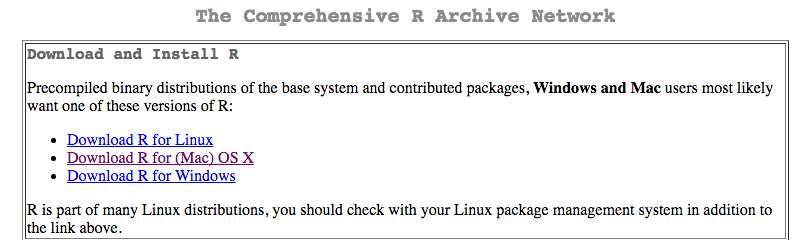
\includegraphics{./media/cran_unipa.png}
\caption{Il server cran ospitato presso l'Università di Padova}
\end{figure}

R è un progetto open source, quindi oltre agli installer è possibile scaricare il codice sorgente di R, ed è possibile apportare modifiche e/o compilarlo personalmente.

Noi scaricheremo invece l'applicazione relativa al vostro sistema operativo (nelle immagine Mac) e procederemo con l'installazione.

La pagina di download permette di scaricare anche versioni meno recenti di R.
Questo può essere importante qualora si usino delle estensioni (chiamate \textbf{\emph{pacchetti}}), che potrebbero non essere state aggiornate per l'ultima versione. Noi considereremo per questo tutorial l'istallazione della versione 3.5.3.

\begin{figure}
\centering
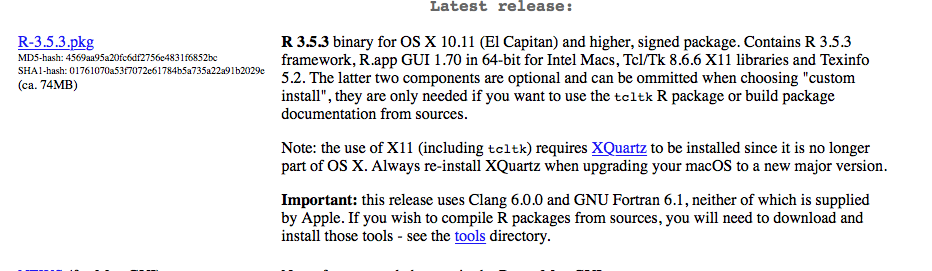
\includegraphics{./media/R353down.png}
\caption{Example image}
\end{figure}

Si noti che l'istallazione su Mac richiede l'istallazione di \href{https://www.xquartz.org/}{XQuartz}

Alcuni computer meno aggiornati potrebbero non supportare la versione più recente (tipo il mio). In tal caso, si consiglia l'istallazione della versione 3.3.3.

\begin{figure}
\centering
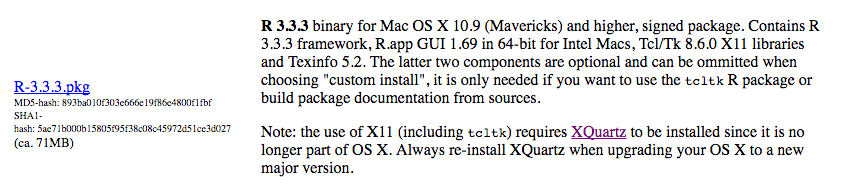
\includegraphics{./media/R330down.png}
\caption{Example image}
\end{figure}

Nel caso in cui si stesse installando R sulla distribuzione linux Ubuntu, è possibile farlo da terminale attraverso i comandi:

\begin{Shaded}
\begin{Highlighting}[]
\FunctionTok{sudo}\NormalTok{ apt-get update}
\FunctionTok{sudo}\NormalTok{ apt-get install r-base}
\end{Highlighting}
\end{Shaded}

Il sito descrive la procedura anche per le altre distribuzioni.

\hypertarget{installare-r-1}{%
\section{Installare R}\label{installare-r-1}}

Nell'istallazione su Mac o Windows si segue la procedura standard una volta scaricati i file.
Per installare R su linux, basta usare i comandi descritti precedentemente per Ubuntu, o utilizzare gli equivalenti per le altre distribuzioni.

\hypertarget{usare-r}{%
\section{Usare R}\label{usare-r}}

Una volta istallato R, è già possibile usarne tutte le funzionalità. Infatti andando in \textbf{Applicazioni} si può già trovare R tra esse. Pigiando la relativa icona si avvia la \textbf{R console}, una interfaccia molto semplice che però permette di usufruire di \textbf{tutte} le potenzialità del software.

\begin{figure}
\centering
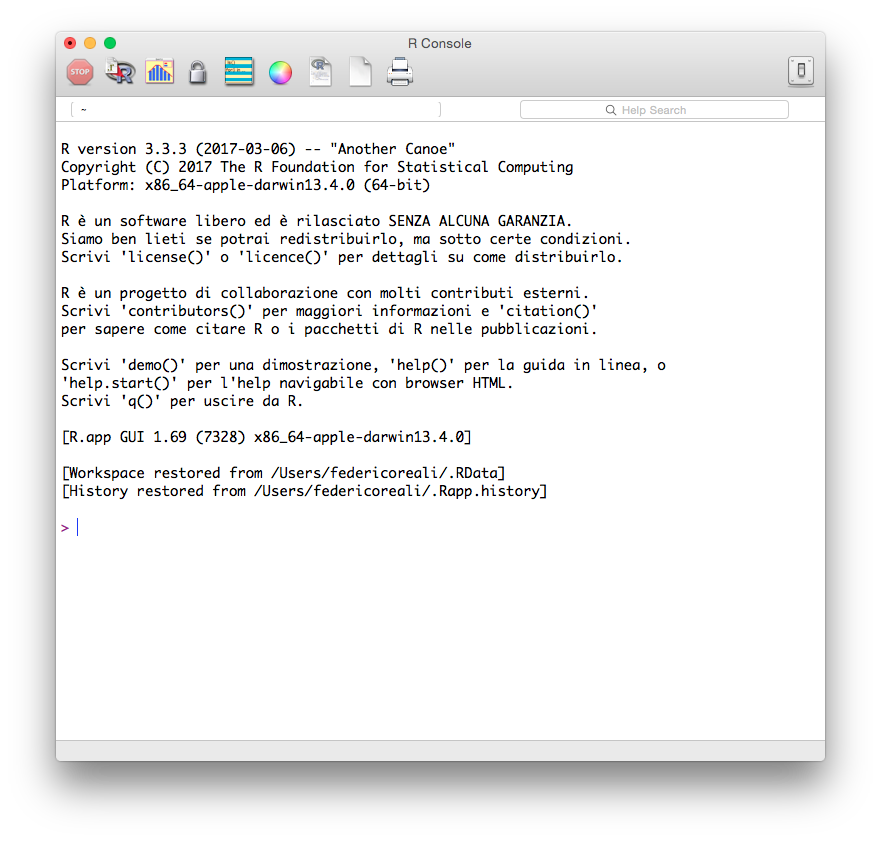
\includegraphics{./media/R_open.png}
\caption{Example image}
\end{figure}

Ad esempio digitando

\begin{Shaded}
\begin{Highlighting}[]
\DecValTok{2}\OperatorTok{+}\DecValTok{2}
\end{Highlighting}
\end{Shaded}

\begin{verbatim}
## [1] 4
\end{verbatim}

oppure

\begin{Shaded}
\begin{Highlighting}[]
\DecValTok{3}\OperatorTok{*}\DecValTok{5}
\end{Highlighting}
\end{Shaded}

\begin{verbatim}
## [1] 15
\end{verbatim}

è possibile utilizzare la console come calcolatrice. Ovviamente questo tipo di uso sfrutta solo una minima parte delle potenzialità del software.

Sebbene tutto quello che faremo sarà possibile farlo anche direttamente da console, noi useremo un software che si interfaccia ad R, ma che presenta un'interfaccia grafica più completa. Tale programma è \href{https://www.rstudio.com/products/rstudio/}{R Studio}.

\hypertarget{installare-r-studio}{%
\section{Installare R Studio}\label{installare-r-studio}}

Come R, anche R Studio è disponibile gratuitamente per utenti singoli, anche se sono previste anche versioni commerciali a pagamento. Inoltre è possibile \href{https://www.rstudio.com/products/rstudio/download2/}{scaricare} pacchetti di installazione sia per Windows, Mac e alcune distribuzioni di Linux.

\begin{figure}
\centering
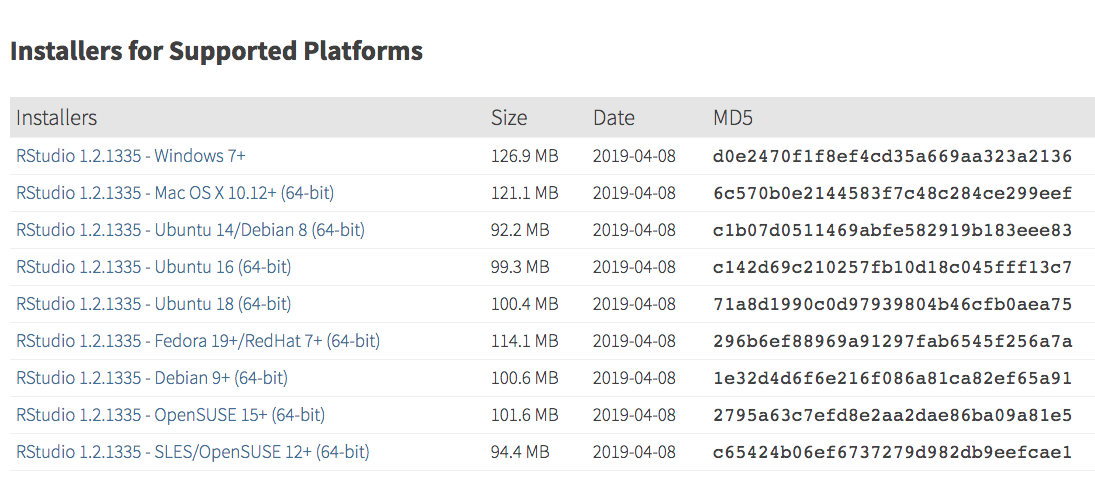
\includegraphics{./media/Rstudio_Versions_2019.png}
\caption{RStudio - Versions}
\end{figure}

Una volta scaricati i pacchetti di installazione, la procedura automatica dovrebbe installare R Studio per tutte le piattaforme (speriamo!).

\hypertarget{usare-r-studio}{%
\section{Usare R Studio}\label{usare-r-studio}}

Una volta installato R Studio, avviamolo e (se l'istallazione è andata a buon fine) dovrebbe apparire la schermata iniziale:

\begin{figure}
\centering
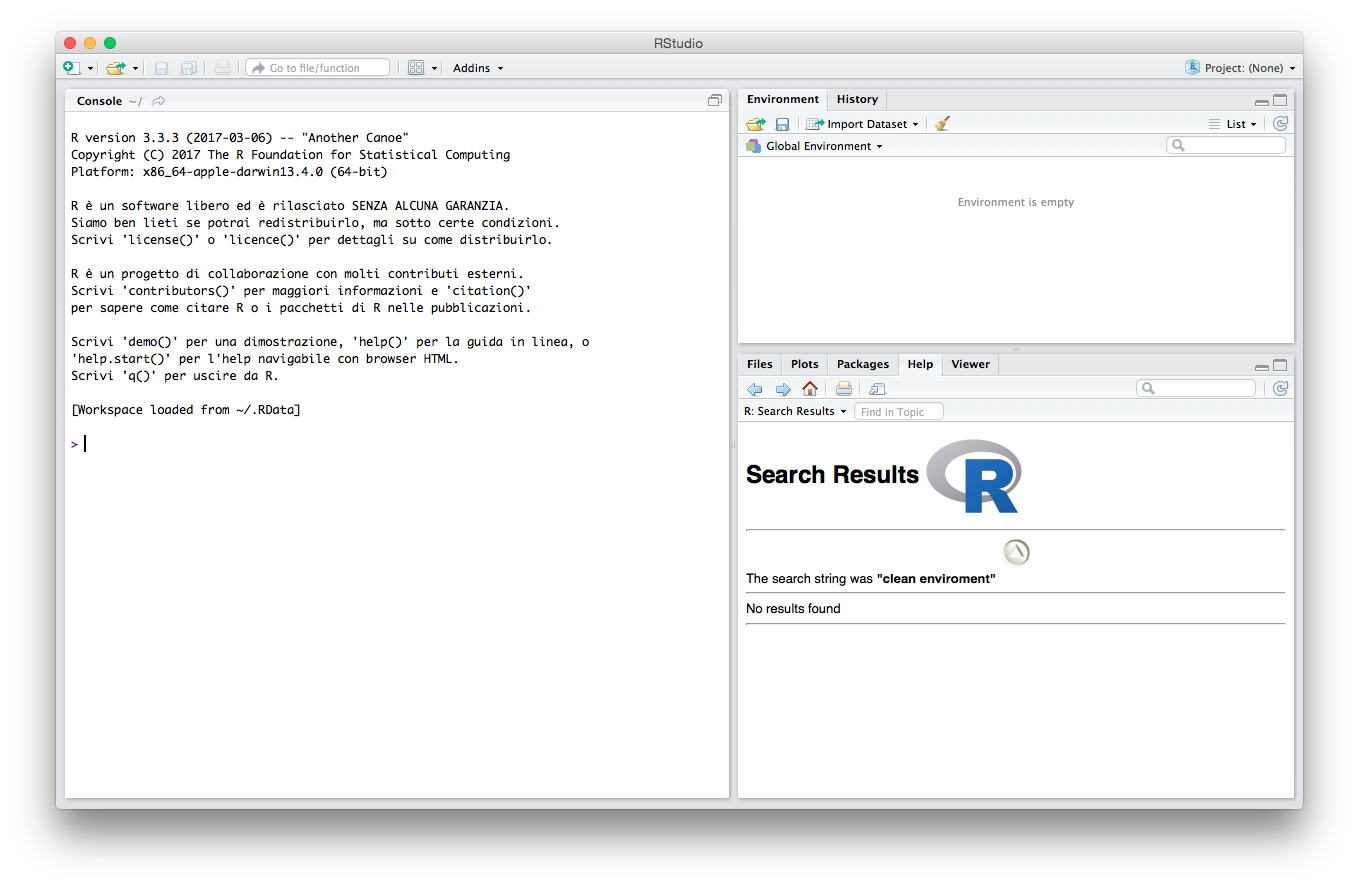
\includegraphics{./media/Rstudio_blank.png}
\caption{RStudio - Versions}
\end{figure}

L'interfaccia grafica si presenta con 3 principali finestre che riportano la console di R (la stessa che abbiamo visto prima singolarmente), la finestra \textbf{Enviroment} e \textbf{History} e quella contenente \textbf{Files}, \textbf{Plots}, \textbf{Packages}, \textbf{Help} e \textbf{Viewer}.

Per prima cosa controlliamo che tutti i pacchetti contenuti nell'installazione siano aggiornati. Selezionando da Tools:

\begin{figure}
\centering
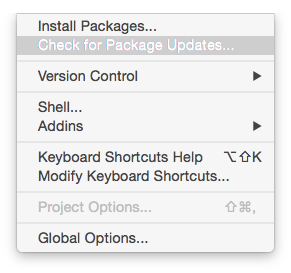
\includegraphics{./media/Rstudio_tool.png}
\caption{RStudio - Versions}
\end{figure}

Se risultano pacchetti da aggiornare, selezionateli tutti e aggiornateli. In caso non vi siano, R Studio vi dovrebbe avvisare.

\hypertarget{cartelle}{%
\subsection{Cartelle}\label{cartelle}}

E' possibile usare degli appositi comandi per capire in quale cartella sta lavorando R. Questo è essenziale se si vuole salvare dei file o leggerne il contenuto.

\begin{Shaded}
\begin{Highlighting}[]
\KeywordTok{getwd}\NormalTok{()}
\end{Highlighting}
\end{Shaded}

\begin{verbatim}
## [1] "/Users/federicoreali/Dropbox/Bonaccorsi/Calcolo delle probabilita e statistica matematica/2019/Rbook/Book"
\end{verbatim}

Questo comando \emph{get working directory} restituisce il path della cartella corrente. R può facilmente leggere o salvare file in questa cartella.

E' possibile impostare una cartella diversa. Ad esempio possiamo creare una cartella relativa al corso di \textbf{Calcolo delle probabilità e statistica matematica (CPeSM)} e possiamo creare lì dentro una cartella chiamata R, dove possiamo salvare i nostri file.

\begin{Shaded}
\begin{Highlighting}[]
\KeywordTok{setwd}\NormalTok{(}\StringTok{'IL-Vostro-path/CPeSM/R/Lezione1'}\NormalTok{)}
\end{Highlighting}
\end{Shaded}

Una volta capito dove siamo e dove dovremmo essere, possiamo iniziare ad usare una delle funzionalità per cui abbiamo scelto R Studio: la possibilità di creare degli script nella stessa interfaccia grafica e di lanciare comandi dagli stessi.

Selezioniamo \textbf{File\textbar{}New File\textbar{}R Script} apriamo in R Studio una nuova finestra che permette di editare (scrivere) uno script.

\begin{figure}
\centering
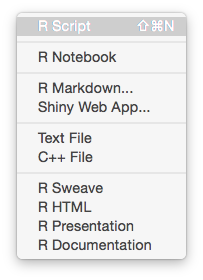
\includegraphics{./media/Rstudio_NewScript.png}
\caption{RStudio - Versions}
\end{figure}

\begin{figure}
\centering
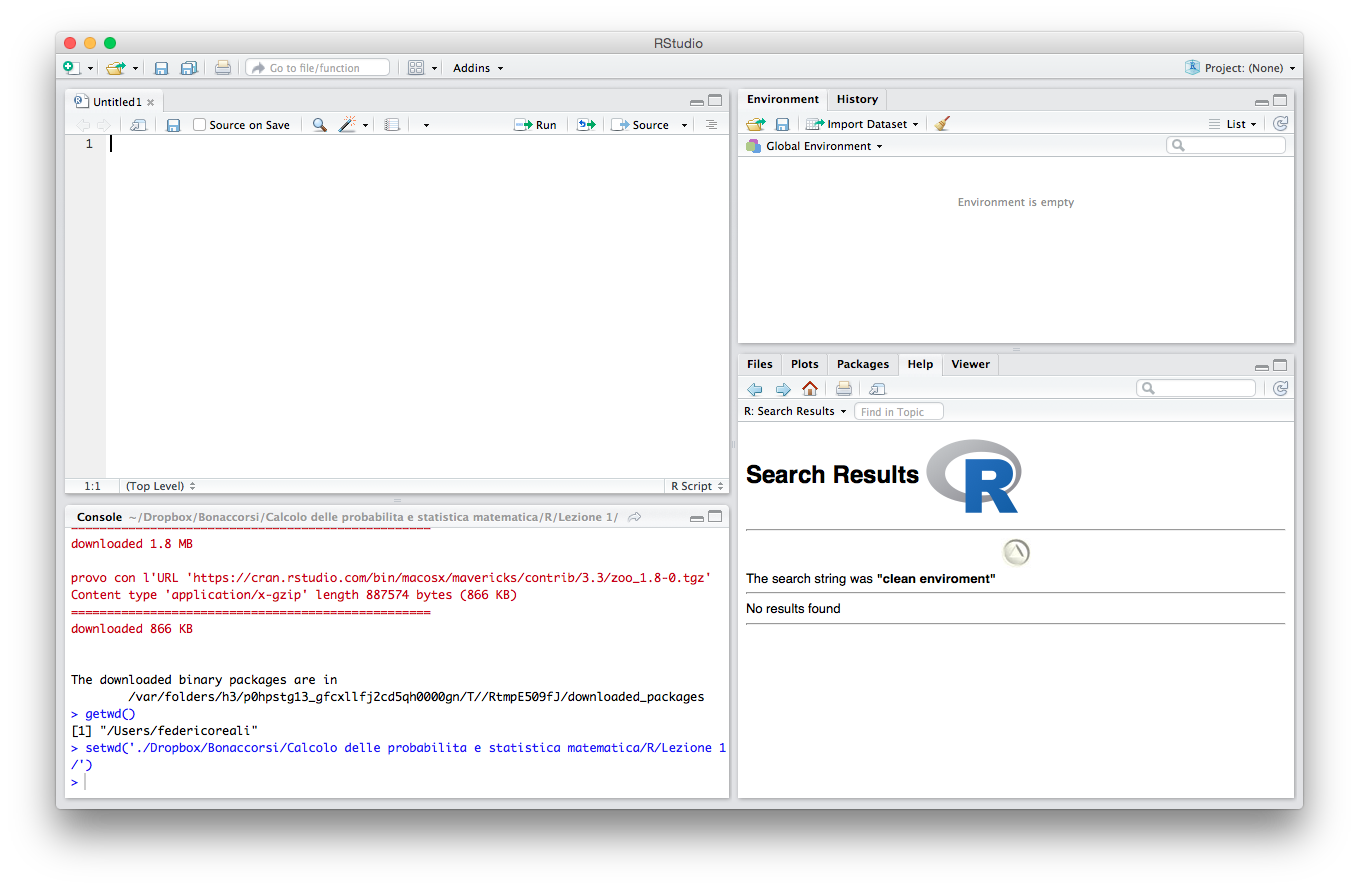
\includegraphics{./media/Rstudio_4tab.png}
\caption{RStudio - Versions}
\end{figure}

Ora non rimane che spendere un po' di tempo a familiarizzare con l'interfaccia e con R!

\hypertarget{link-utili}{%
\section{Link utili}\label{link-utili}}

\begin{itemize}
\tightlist
\item
  A questo \href{https://cran.r-project.org/doc/contrib/Mineo-dispensaR.pdf}{link} è possibile reperire delle utili dispense sull'uso di R.
\item
  A questo \href{https://cran.r-project.org/doc/contrib/Frascati-FormularioStatisticaR.pdf}{link} è possibile reperire un utile formulario che descrive moltissimi comandi di R.
\end{itemize}

\hypertarget{primi-comandi-di-r}{%
\chapter{Primi comandi di R}\label{primi-comandi-di-r}}

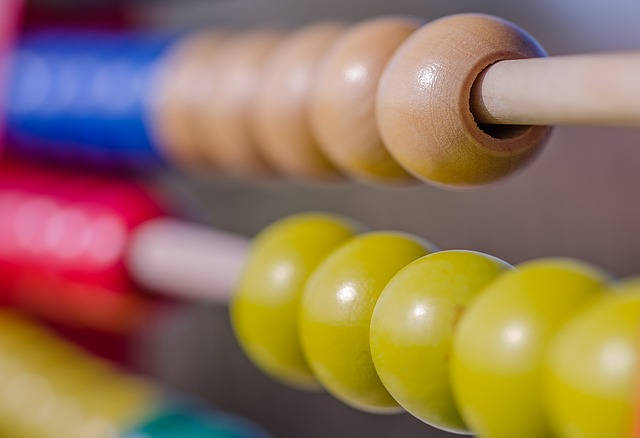
\includegraphics{./media/abacus.jpg}

\hypertarget{operazioni-aritmetiche}{%
\section{Operazioni Aritmetiche}\label{operazioni-aritmetiche}}

Come abbiamo già visto è possibile usare R per svolgere operazioni matematiche, usando i simboli standard.

Ad esempio, l'uso di \texttt{+} più tra due numeri farà comparire la loro somma.
In modo analogo è possibile farne la differenza (\texttt{-}), il prodotto (\texttt{*}) e la divisione(\texttt{/}).

\begin{Shaded}
\begin{Highlighting}[]
\DecValTok{2}\OperatorTok{+}\DecValTok{2} 
\end{Highlighting}
\end{Shaded}

\begin{verbatim}
## [1] 4
\end{verbatim}

\begin{Shaded}
\begin{Highlighting}[]
\DecValTok{2-2}
\end{Highlighting}
\end{Shaded}

\begin{verbatim}
## [1] 0
\end{verbatim}

\begin{Shaded}
\begin{Highlighting}[]
\DecValTok{2}\OperatorTok{*}\DecValTok{2}
\end{Highlighting}
\end{Shaded}

\begin{verbatim}
## [1] 4
\end{verbatim}

\begin{Shaded}
\begin{Highlighting}[]
\DecValTok{2}\OperatorTok{/}\DecValTok{2}
\end{Highlighting}
\end{Shaded}

\begin{verbatim}
## [1] 1
\end{verbatim}

Le potenze si possono esprimere usando il simbolo \texttt{\^{}}. Lo stesso simbolo si può utilizzare per il calcolo delle radici, anche se è possibile richiamare la radice quadrata usando il comando \texttt{sqrt()}. Si noti che tale funzione accetta anche valori complessi.

Per la divisione intera tra due numeri è possibile usare il simbolo \texttt{\%/\%}, mentre \texttt{\%\%} restituisce il resto di tale divisione.

Un altro comando di base che può risultare utile è il calcolo del valore assoluto ottenuto con il comando \texttt{abs()}.

In modo analogo sono già definite alcune delle funzioni che sono alla base dei calcoli matematici più frequenti. Le vedremo nei prossimi paragrafi.

\hypertarget{esponenziale-e-logaritmi}{%
\section{Esponenziale e logaritmi}\label{esponenziale-e-logaritmi}}

E' possibile calcolare i valori della funzione esponenziale usando il comando \texttt{exp()} mentre per il calcolo dei logaritmi è possibile usare più funzioni:
\texttt{log(),\ log10()} e \texttt{log2()} che restituiscono il logaritmo naturale, base 10 e base 2 rispettivamente. Il comando \texttt{log()} permette anche di specificare una base differente da \textbf{\emph{e}}, che è quella di default. Ad esempio, \texttt{log(\ 5\ ,\ base\ =\ 3)} restituisce il logaritmo in base 3 di 5.

\hypertarget{funzioni-trigonometriche}{%
\section{Funzioni Trigonometriche}\label{funzioni-trigonometriche}}

Le principali funzioni trigonometriche sono già implementate in R e si possono richiamare usando i comandi elencati sotto, i cui nomi richiamano le funzioni stesse. Va notato che l'input di queste funzioni è atteso in radianti, \textbf{non gradi}.

\begin{Shaded}
\begin{Highlighting}[]
\KeywordTok{sin}\NormalTok{() }\CommentTok{# seno}
\KeywordTok{cos}\NormalTok{() }\CommentTok{# cosen}
\KeywordTok{tan}\NormalTok{() }\CommentTok{# tangente}
\end{Highlighting}
\end{Shaded}

E' possibile utilizzare le stesse funzioni ma con desinenza \textbf{\emph{pi}} (\texttt{sinpi()}, \texttt{cospi()} e \texttt{tanpi()}) se si intende considerare dei multipli di pi-greco.

Anche le funzioni inverse sono già implementate e si possono richiamare con i comandi \texttt{acos(),\ asin(),\ atan()}.

\hypertarget{assegnazione-e-vettori}{%
\section{Assegnazione e vettori}\label{assegnazione-e-vettori}}

Fin ora abbiamo usato R per calcolare dei singoli valori, in modo analogo a come avremmo usato una calcolatrice. Tuttavia R permette di fare molto di più.

Come primo passo per scoprirne le potenzialità vedremo la possibilità di assegnare valori e di richiamarli successivamente, così come di lavorare con vettori o matrici, invece che con singoli valori.

Questa parte, così come alcune successive sono anche coperte dalle utili \href{https://cran.r-project.org/doc/contrib/Mineo-dispensaR.pdf}{dispense}, di cui ho già consigliato la lettura.

E' possibile assegnare un valore ad una variabile usando la freccina \texttt{-\textgreater{}}. Stesso risultato si può ottenere usando \texttt{=} oppure \texttt{assign()}, tuttavia il primo è decisamente il comando più usato e di più facile lettura. \href{http://stackoverflow.com/questions/1741820/assignment-operators-in-r-and}{Qui} è possibile leggere una discussione sulle differenze nell'uso di \texttt{=} o di \texttt{-\textgreater{}}.

\begin{Shaded}
\begin{Highlighting}[]
\NormalTok{x  <-}\StringTok{ }\DecValTok{6}
\end{Highlighting}
\end{Shaded}

Usando il precedente comando viene assegnato il valore 6 alla variabile x. In questo modo è possibile richiamarla successivamente, così come è possibile scrivere espressioni più complesse che coinvolgono x a prescindere dal suo valore. Questo sarà particolarmente utile se dovremo definire delle funzioni a cui è possibile passare per argomento diversi valori.
Si noti che il comando \texttt{6\ -\textgreater{}\ x} produce gli stessi risultati del precedente.

Oltre ad assegnare un singolo valore, è possibile considerati dei vettori.
Il comando

\begin{Shaded}
\begin{Highlighting}[]
\NormalTok{y <-}\StringTok{ }\KeywordTok{c}\NormalTok{(}\DecValTok{1}\NormalTok{,}\DecValTok{2}\NormalTok{,}\DecValTok{3}\NormalTok{,}\DecValTok{4}\NormalTok{)}
\NormalTok{y[}\DecValTok{1}\NormalTok{]}
\end{Highlighting}
\end{Shaded}

\begin{verbatim}
## [1] 1
\end{verbatim}

assegna a y i valori contenuti nel comando \texttt{c()}. Tale comando combina i valori in un vettore colonna ( ma viene visualizzato come riga). L'accesso ai vettori avviene attraverso indicandone il nome, seguito da parentesi quadre. Ovviamente è possibile svolgere operazioni aritmetiche anche tra vettori, usando la stessa sintassi vista prima.
Di default R considera operazioni puntuali tra vettori, cioè l'operazione richiesta viene svolta entrata per entrata. Questo richiede le dimensioni siano le stesse. Qualora non lo fossero, il contenuto del vettore più piccolo viene ripetuto un numero di volte sufficienti da rendere possibile l'operazione. Questo viene anche segnalato da un warning.

E' possibile ottenere le dimensioni di un vettore usando il comando \texttt{length()}.

Un comando utile tra vettori è \texttt{t()} che traspone il vettore passato per argomento.

\begin{Shaded}
\begin{Highlighting}[]
\NormalTok{z <-}\StringTok{ }\KeywordTok{t}\NormalTok{(y)}
\NormalTok{y}
\end{Highlighting}
\end{Shaded}

\begin{verbatim}
## [1] 1 2 3 4
\end{verbatim}

\begin{Shaded}
\begin{Highlighting}[]
\KeywordTok{print}\NormalTok{(z)}
\end{Highlighting}
\end{Shaded}

\begin{verbatim}
##      [,1] [,2] [,3] [,4]
## [1,]    1    2    3    4
\end{verbatim}

\begin{Shaded}
\begin{Highlighting}[]
\NormalTok{z}
\end{Highlighting}
\end{Shaded}

\begin{verbatim}
##      [,1] [,2] [,3] [,4]
## [1,]    1    2    3    4
\end{verbatim}

Chiamare una variabile senza indicare operazioni ne permette la stampa a video. Inserendo l'assegnazione tra parentesi tonde si ottiene lo stesso risultato. Anche il comando \texttt{print()} permetta la stampa a video. Inoltre questo comando, diversamente dai precedenti, permette di mostrare l'output anche quando è chiamata dentro una funzione o uno script.

Dal comando precedente vediamo che y e z hanno stessi valori ma dimensioni diverse. Tuttavia R permette di svolgere operazioni matematiche su di essi senza warning o errori.

Per svolgere operazioni tra vettori, come il prodotto righe per colonne si può considerare il comando \texttt{\%*\%}. In questo caso il risultato dipende dall'ordine.

\begin{Shaded}
\begin{Highlighting}[]
\NormalTok{y }\OperatorTok\StringTok{ }\NormalTok{z}
\end{Highlighting}
\end{Shaded}

\begin{verbatim}
##      [,1] [,2] [,3] [,4]
## [1,]    1    2    3    4
## [2,]    2    4    6    8
## [3,]    3    6    9   12
## [4,]    4    8   12   16
\end{verbatim}

\begin{Shaded}
\begin{Highlighting}[]
\NormalTok{z }\OperatorTok\StringTok{ }\NormalTok{y}
\end{Highlighting}
\end{Shaded}

\begin{verbatim}
##      [,1]
## [1,]   30
\end{verbatim}

\hypertarget{sequenze}{%
\section{Sequenze}\label{sequenze}}

Nel caso si debba indicare una successione di valori è possibile farlo senza indicarli espressamente tutti, purché essi siano una sequenza regolare.

Ad esempio con \texttt{a:b} possiamo usare i due punti per indicare una sequenza di valori con passo 1 da \emph{a} fino a \emph{b} . Per indicare un passo diverso possiamo usare il comando \texttt{seq(a,b,passo)} che produrrà una sequenza di elementi da \emph{a} fino a \emph{b} distanziati di un valore uguale al \emph{passo} indicato. Se il passo viene omesso è considerato 1 di default.

Per tutte le funzioni è possibile accedere all'help di R usando il comando \texttt{help(Nome\_funzione)}. Leggendo l'help di \texttt{seq()} vediamo ad esempio che possiamo anche indicare in ordine diverso i parametri, a patto di specificarli usando il nome indicato nell'help. Ad esempio \texttt{seq(to\ =\ b,\ by\ =\ passo,\ from\ =\ a)} restituisce lo stesso output di \texttt{seq(a,b,passo)}.

Inoltre è possibile ripetere un valore o un vettore usando il comando \texttt{rep()}, ad esempio \texttt{rep(1,5)} restituisce cinque volte il valore 1. Nel caso di un vettore, il comando ripeterà 5 volte il vettore.

\hypertarget{operazioni-su-vettori}{%
\section{Operazioni su vettori}\label{operazioni-su-vettori}}

Oltre alle operazioni che abbiamo già visto esistono altre funzioni di R appositamente pensate per i vettori. Ad esempio le funzioni \texttt{min} e \texttt{max} restituiscono, rispettivamente, il minimo ed il massimo valore contenuto in un vettore. Per accedere alla posizione di tali valori si combinano i precedenti comandi con \texttt{which}. Ad esempio

\begin{Shaded}
\begin{Highlighting}[]
\NormalTok{x <-}\StringTok{ }\KeywordTok{c}\NormalTok{(}\DecValTok{3}\NormalTok{, }\DecValTok{5}\NormalTok{, }\DecValTok{7}\NormalTok{, }\DecValTok{1}\NormalTok{, }\DecValTok{3}\NormalTok{, }\DecValTok{3}\NormalTok{, }\DecValTok{9}\NormalTok{, }\DecValTok{8}\NormalTok{)}
\KeywordTok{min}\NormalTok{(x)}
\end{Highlighting}
\end{Shaded}

\begin{verbatim}
## [1] 1
\end{verbatim}

\begin{Shaded}
\begin{Highlighting}[]
\KeywordTok{which.min}\NormalTok{(x)}
\end{Highlighting}
\end{Shaded}

\begin{verbatim}
## [1] 4
\end{verbatim}

\begin{Shaded}
\begin{Highlighting}[]
\KeywordTok{max}\NormalTok{(x)}
\end{Highlighting}
\end{Shaded}

\begin{verbatim}
## [1] 9
\end{verbatim}

\begin{Shaded}
\begin{Highlighting}[]
\KeywordTok{which.max}\NormalTok{(x)}
\end{Highlighting}
\end{Shaded}

\begin{verbatim}
## [1] 7
\end{verbatim}

Altre funzioni molto utili per lavorare con i vettori sono la funzione \texttt{sum()} che calcola la somma di tutti gli elementi di un vettore e la funzione \texttt{diff()}
che calcola la differenza di un valore da uno dei precedenti (è possibile indicare quanto prima ``guardare'').

\begin{Shaded}
\begin{Highlighting}[]
\KeywordTok{sum}\NormalTok{(x)}
\end{Highlighting}
\end{Shaded}

\begin{verbatim}
## [1] 39
\end{verbatim}

\begin{Shaded}
\begin{Highlighting}[]
\KeywordTok{diff}\NormalTok{(x)}
\end{Highlighting}
\end{Shaded}

\begin{verbatim}
## [1]  2  2 -6  2  0  6 -1
\end{verbatim}

\begin{Shaded}
\begin{Highlighting}[]
\KeywordTok{diff}\NormalTok{(x,}\DecValTok{2}\NormalTok{)}
\end{Highlighting}
\end{Shaded}

\begin{verbatim}
## [1]  4 -4 -4  2  6  5
\end{verbatim}

\hypertarget{operatori-relazionali-e-logici}{%
\section{Operatori relazionali e logici}\label{operatori-relazionali-e-logici}}

R ci permette anche di valutare espressioni relazionali o logiche. Il loro risultato sarà un valore logico indicato con TRUE o FALSE.

\begin{Shaded}
\begin{Highlighting}[]
\DecValTok{6} \OperatorTok{>}\StringTok{ }\DecValTok{10}
\end{Highlighting}
\end{Shaded}

\begin{verbatim}
## [1] FALSE
\end{verbatim}

\begin{Shaded}
\begin{Highlighting}[]
\DecValTok{6} \OperatorTok{<=}\StringTok{ }\DecValTok{10}
\end{Highlighting}
\end{Shaded}

\begin{verbatim}
## [1] TRUE
\end{verbatim}

\begin{Shaded}
\begin{Highlighting}[]
\NormalTok{is_bigger <-}\StringTok{ }\DecValTok{6}\OperatorTok{>}\StringTok{ }\DecValTok{10}
\NormalTok{is_bigger}
\end{Highlighting}
\end{Shaded}

\begin{verbatim}
## [1] FALSE
\end{verbatim}

\begin{Shaded}
\begin{Highlighting}[]
\KeywordTok{as.integer}\NormalTok{(is_bigger)}
\end{Highlighting}
\end{Shaded}

\begin{verbatim}
## [1] 0
\end{verbatim}

R permette di valutare diverse espressioni relazionari, oltre a maggiore (uguale) o minore (uguale). Ad esempio è possibile valutare se due valori o variabili siano diversi \texttt{!=} o uguali \texttt{==}. Questo può essere particolarmente utile quando si definiscono delle funzioni proprie e si valuta se una condizione è soddisfatta.

R permette anche di valutare gli operatori logici \texttt{\&} (and), \texttt{\textbar{}} (or), \texttt{xor} e \texttt{!} (not).

Questi operatori possono essere valutati sia su vettori logici, che di numeri qualsiasi. Nel secondo caso, tuttavia, tutto ciò che è diverso da zero conterà come TRUE, e solo lo 0 conterà come FALSE. Nel caso in cui si definiscano dei vettori misti (dove sono presenti sia valori logici che interi/reali/complessi), verranno tutti convertiti nel formato numerico presente.

\hypertarget{matrici}{%
\section{Matrici}\label{matrici}}

Come abbiamo visto i vettori sono considerati in generale vettori riga, e non è possibile generare una matrice usando il comando \texttt{c()}.

Tuttavia le matrici esistono e si possono definire usando la funzione \texttt{cbind()} che unisce i vettori passati come argomento in una matrice dove i vettori argomento sono le colonne. La funzione \texttt{rbind()} ha la stessa funzione, ma i vettori passati come argomento saranno le righe della matrice. In tutti e due i casi, i vettori passati come argomento devono avere stessa dimensione (no uno riga e uno colonna). La funzione \texttt{dim()} restituisce le dimensioni dell'oggetto passato come argomento. La funzione \texttt{length()} (che avevamo visto con i vettori) ci restituisce il \emph{prodotto} delle dimensioni.

\begin{Shaded}
\begin{Highlighting}[]
\NormalTok{a <-}\StringTok{ }\KeywordTok{cbind}\NormalTok{(}\KeywordTok{c}\NormalTok{(}\DecValTok{1}\NormalTok{, }\DecValTok{2}\NormalTok{, }\DecValTok{3}\NormalTok{), }\KeywordTok{c}\NormalTok{(}\DecValTok{4}\NormalTok{, }\DecValTok{5}\NormalTok{, }\DecValTok{6}\NormalTok{))}
\KeywordTok{dim}\NormalTok{(a)}
\end{Highlighting}
\end{Shaded}

\begin{verbatim}
## [1] 3 2
\end{verbatim}

\begin{Shaded}
\begin{Highlighting}[]
\NormalTok{b <-}\StringTok{ }\KeywordTok{rbind}\NormalTok{(}\KeywordTok{c}\NormalTok{(}\DecValTok{1}\NormalTok{, }\DecValTok{2}\NormalTok{, }\DecValTok{3}\NormalTok{), }\KeywordTok{c}\NormalTok{(}\DecValTok{4}\NormalTok{, }\DecValTok{5}\NormalTok{, }\DecValTok{6}\NormalTok{))}
\KeywordTok{dim}\NormalTok{(b)}
\end{Highlighting}
\end{Shaded}

\begin{verbatim}
## [1] 2 3
\end{verbatim}

\begin{Shaded}
\begin{Highlighting}[]
\NormalTok{a}
\end{Highlighting}
\end{Shaded}

\begin{verbatim}
##      [,1] [,2]
## [1,]    1    4
## [2,]    2    5
## [3,]    3    6
\end{verbatim}

\begin{Shaded}
\begin{Highlighting}[]
\NormalTok{b}
\end{Highlighting}
\end{Shaded}

\begin{verbatim}
##      [,1] [,2] [,3]
## [1,]    1    2    3
## [2,]    4    5    6
\end{verbatim}

E' possibile variare la dimensione di un oggetto usando gli stessi comandi \texttt{length} e \texttt{dim} come assegnazioni.

\begin{Shaded}
\begin{Highlighting}[]
\KeywordTok{dim}\NormalTok{(a) <-}\StringTok{ }\KeywordTok{c}\NormalTok{(}\DecValTok{2}\NormalTok{,}\DecValTok{3}\NormalTok{)}
\NormalTok{a}
\end{Highlighting}
\end{Shaded}

\begin{verbatim}
##      [,1] [,2] [,3]
## [1,]    1    3    5
## [2,]    2    4    6
\end{verbatim}

Il comando precedente cambia la forma della matrice, secondo la forma indicata. Tali comandi vanno comunque usati con attenzione, visto che non si ha controllo su come il contenuto verrà ridistribuito.

Altra utile funzione per creare matrici è la funzione \texttt{array()} che chiede di specificare gli elementi della matrice e le dimensioni. Risultato analogo si può otenere con la funzione \texttt{matrix(elementi,\ num\ righe,\ num\ colonne)}. Si noti che con \texttt{array()} è possibile definire strutture con più di due dimensioni.

Gli elementi una matrice si accedono usando le parentesi quadre, indicando la posizione dell'elemento.

\begin{Shaded}
\begin{Highlighting}[]
\NormalTok{a[}\DecValTok{2}\NormalTok{,}\DecValTok{3}\NormalTok{]}
\end{Highlighting}
\end{Shaded}

\begin{verbatim}
## [1] 6
\end{verbatim}

Se si intende selezionare un'intera riga o colonna, basta lasciare vuoto tale campo. Per esempio \texttt{a{[}1,{]}} restitusce l'intera prima riga.

Alcune funzioni come \texttt{contour(),\ persp(),\ image()} permettono di ottenere dei grafici, partendo da matrici.

\hypertarget{stringhe-vettori-di-caratteri}{%
\section{Stringhe (vettori di caratteri)}\label{stringhe-vettori-di-caratteri}}

R permette di manipolare anche vettori di caratteri, o stringhe, che possono essere salvati anche come vettori. Le stringhe vengono delimitate da doppie virgolette \texttt{"\ "} (o anche semplici virgolette \texttt{\textquotesingle{}\ \textquotesingle{}}).

\begin{Shaded}
\begin{Highlighting}[]
\NormalTok{nomi <-}\StringTok{ }\KeywordTok{c}\NormalTok{(}\StringTok{"Francesco"}\NormalTok{, }\StringTok{"Sofia"}\NormalTok{, }\StringTok{"Alessandro"}\NormalTok{)}
\NormalTok{nomi[}\DecValTok{1}\NormalTok{]}
\end{Highlighting}
\end{Shaded}

\begin{verbatim}
## [1] "Francesco"
\end{verbatim}

\begin{Shaded}
\begin{Highlighting}[]
\NormalTok{nomi_e_numeri <-}\StringTok{ }\KeywordTok{c}\NormalTok{(}\StringTok{"Francesco"}\NormalTok{, }\StringTok{"Sofia"}\NormalTok{, }\StringTok{"Alessandro"}\NormalTok{, }\DecValTok{45}\NormalTok{)}
\end{Highlighting}
\end{Shaded}

In R non possono convivere nello stesso array caratteri e numeri. Se ad esempio nell'assegnazione indichiamo nomi e numeri, questi ultimi verranno convertiti in caratteri.

Una funzione molto utile per maneggiare stringhe, ma anche altri risultati, è la funzione \texttt{paste()} che concatena dei vettori dopo averli trasformati in stringhe.

\begin{Shaded}
\begin{Highlighting}[]
\KeywordTok{paste}\NormalTok{(}\DecValTok{1}\OperatorTok{:}\DecValTok{12}\NormalTok{) }
\end{Highlighting}
\end{Shaded}

\begin{verbatim}
##  [1] "1"  "2"  "3"  "4"  "5"  "6"  "7"  "8"  "9"  "10" "11" "12"
\end{verbatim}

\begin{Shaded}
\begin{Highlighting}[]
\NormalTok{(nth <-}\StringTok{ }\KeywordTok{paste0}\NormalTok{(}\DecValTok{1}\OperatorTok{:}\DecValTok{12}\NormalTok{, }\KeywordTok{c}\NormalTok{(}\StringTok{"st"}\NormalTok{, }\StringTok{"nd"}\NormalTok{, }\StringTok{"rd"}\NormalTok{, }\KeywordTok{rep}\NormalTok{(}\StringTok{"th"}\NormalTok{, }\DecValTok{9}\NormalTok{))))}
\end{Highlighting}
\end{Shaded}

\begin{verbatim}
##  [1] "1st"  "2nd"  "3rd"  "4th"  "5th"  "6th"  "7th"  "8th"  "9th"  "10th"
## [11] "11th" "12th"
\end{verbatim}

Questa funzione può essere molto utile, ad esempio, se si devono creare vettori di nomi per delle variabili.

Per capire il tipo di dati contenuto in un vettore possiamo usare il comando \texttt{typeof()} o \texttt{class()}.

\hypertarget{liste-e-data-frame}{%
\section{Liste e data frame}\label{liste-e-data-frame}}

Possiamo pensare ad una matrice come ad un metodo efficace per immagazzinare informazioni numeriche, ed è così! Però se il tipo di informazioni che dobbiamo immagazzinare è misto, ad esempio contiene sia numeri che caratteri, la loro efficienza viene meno e si possono preferire altri metodi.

Una lista è un insieme ordinato di oggetti. Si possono definire liste usando il comando \texttt{list()}.

\begin{Shaded}
\begin{Highlighting}[]
\NormalTok{c <-}\StringTok{ }\KeywordTok{list}\NormalTok{(}\DataTypeTok{destinazione =} \KeywordTok{c}\NormalTok{(}\StringTok{"London"}\NormalTok{, }\StringTok{"Madrid"}\NormalTok{), }\DataTypeTok{compagnia =} \KeywordTok{c}\NormalTok{(}\StringTok{"Ryanair"}\NormalTok{, }\StringTok{"EasyJet"}\NormalTok{), }\DataTypeTok{costo =} \KeywordTok{c}\NormalTok{(}\DecValTok{60}\NormalTok{, }\DecValTok{80}\NormalTok{), }\DataTypeTok{valuta =} \KeywordTok{c}\NormalTok{(}\StringTok{"£"}\NormalTok{, }\StringTok{"$"}\NormalTok{) )}
\end{Highlighting}
\end{Shaded}

Si può accedere al contenuto di una lista sia per posizione con le doppie parentesi \texttt{c{[}{[}2{]}{]}} oppure per nome \texttt{c{[}{[}"compagnia"{]}{]}} o \texttt{c\$compagnia}. Tutti i precedenti comandi restituiscono il contenuto della lista definito da \emph{compagnia}. Se vogliamo accedere direttamente ad un elemento possiamo usare indifferentemente i comandi \texttt{c{[}{[}2{]}{]}{[}2{]}}, \texttt{c{[}{[}"compagnia"{]}{]}{[}2{]}} o \texttt{c\$compagnia{[}2{]}}.

\hypertarget{data-frame}{%
\subsection{Data frame}\label{data-frame}}

Un'altra struttura dati che permette di immagazzinate dati di tipo misto sono i \emph{data frame}. Questa struttura è di gran lunga la più usata per leggere e manipolare dati in R.

I \emph{data frame} sono liste di tipo ``data.frame'' contenenti variabili con lo stesso numero di righe, il cui identificativo è univoco.

\begin{Shaded}
\begin{Highlighting}[]
\NormalTok{L3 <-}\StringTok{ }\NormalTok{LETTERS[}\DecValTok{1}\OperatorTok{:}\DecValTok{3}\NormalTok{]}
\NormalTok{fac <-}\StringTok{ }\KeywordTok{sample}\NormalTok{(L3, }\DecValTok{10}\NormalTok{, }\DataTypeTok{replace =} \OtherTok{TRUE}\NormalTok{)}
\NormalTok{(d <-}\StringTok{ }\KeywordTok{data.frame}\NormalTok{(}\DataTypeTok{x =} \DecValTok{1}\NormalTok{, }\DataTypeTok{y =} \DecValTok{1}\OperatorTok{:}\DecValTok{10}\NormalTok{, }\DataTypeTok{fac =}\NormalTok{ fac))}
\end{Highlighting}
\end{Shaded}

\begin{verbatim}
##    x  y fac
## 1  1  1   B
## 2  1  2   B
## 3  1  3   C
## 4  1  4   C
## 5  1  5   C
## 6  1  6   C
## 7  1  7   B
## 8  1  8   A
## 9  1  9   B
## 10 1 10   A
\end{verbatim}

\begin{Shaded}
\begin{Highlighting}[]
\KeywordTok{data.frame}\NormalTok{(}\DecValTok{1}\NormalTok{, }\DecValTok{1}\OperatorTok{:}\DecValTok{10}\NormalTok{, fac)}
\end{Highlighting}
\end{Shaded}

\begin{verbatim}
##    X1 X1.10 fac
## 1   1     1   B
## 2   1     2   B
## 3   1     3   C
## 4   1     4   C
## 5   1     5   C
## 6   1     6   C
## 7   1     7   B
## 8   1     8   A
## 9   1     9   B
## 10  1    10   A
\end{verbatim}

\begin{Shaded}
\begin{Highlighting}[]
\CommentTok{## The "same" with automatic column names:}
\KeywordTok{data.frame}\NormalTok{(}\KeywordTok{rep}\NormalTok{(}\DecValTok{1}\NormalTok{,}\DecValTok{10}\NormalTok{), }\DecValTok{1}\OperatorTok{:}\DecValTok{10}\NormalTok{, fac)}
\end{Highlighting}
\end{Shaded}

\begin{verbatim}
##    rep.1..10. X1.10 fac
## 1           1     1   B
## 2           1     2   B
## 3           1     3   C
## 4           1     4   C
## 5           1     5   C
## 6           1     6   C
## 7           1     7   B
## 8           1     8   A
## 9           1     9   B
## 10          1    10   A
\end{verbatim}

\begin{Shaded}
\begin{Highlighting}[]
\KeywordTok{data.frame}\NormalTok{(}\DecValTok{1}\NormalTok{, }\DecValTok{1}\OperatorTok{:}\DecValTok{10}\NormalTok{, }\KeywordTok{sample}\NormalTok{(L3, }\DecValTok{10}\NormalTok{, }\DataTypeTok{replace =} \OtherTok{TRUE}\NormalTok{))}
\end{Highlighting}
\end{Shaded}

\begin{verbatim}
##    X1 X1.10 sample.L3..10..replace...TRUE.
## 1   1     1                              C
## 2   1     2                              B
## 3   1     3                              C
## 4   1     4                              B
## 5   1     5                              A
## 6   1     6                              C
## 7   1     7                              B
## 8   1     8                              A
## 9   1     9                              A
## 10  1    10                              C
\end{verbatim}

\hypertarget{tidy-data-please}{%
\subsection{Tidy data, please!}\label{tidy-data-please}}

\begin{quote}
A huge amount of effort is spent cleaning data to get it ready for
analysis, but there has been little research on how to make data cleaning as easy and effective as possible. This paper tackles a small, but important, component of data cleaning: data tidying. \textbf{Tidy datasets} are easy to manipulate, model and visualize, and \textbf{have a specific structure: each variable is a column, each observation is a row, and each type of observational unit is a table}. This framework makes it easy to tidy messy datasets because only a small set of tools are needed to deal with a wide range of un-tidy datasets. This structure also makes it easier to develop tidy tools for data analysis, tools that both input and output tidy datasets. The advantages of a consistent data structure and matching tools are demonstrated with a case study free from mundane data manipulation chores.

 \href{https://www.jstatsoft.org/article/view/v059i10}{Tidy data} - Hadley Wickham
\end{quote}

Visto l'importanza dei dati nel mondo moderno e l'innegabile importanza del tempo nella nostra società, evitiamo di perdere troppo tempo a risistemare i nostri dati e cerchiamo di uniformarci ai \emph{tidy data} da quando creiamo un dataset in poi. Questo ci farà risparmiare molto tempo e migliorerà la ripetibilità delle nostre analisi!

\hypertarget{programmazione-in-r}{%
\section{Programmazione in R}\label{programmazione-in-r}}

R permette di eseguire comandi che permetto l'iterazione, la valutazione di espressioni condizionali e la definizione di funzioni.

\hypertarget{condizioni-if}{%
\subsection{Condizioni: if}\label{condizioni-if}}

\begin{Shaded}
\begin{Highlighting}[]
\ControlFlowTok{if}\NormalTok{ (condizione) comando1 }\ControlFlowTok{else}\NormalTok{ comando2}
\CommentTok{#Oppure}
\KeywordTok{ifelse}\NormalTok{(condizione,comando1,comando2)}
\end{Highlighting}
\end{Shaded}

La prima espressione verifica una \emph{condizione} \textbf{solo} su singolo elemento. Al contrario, il comando \texttt{ifelse} permette di vettorializzare il controllo. Se la \emph{condizione} è va valutata su un vettore, il comando \texttt{ifelse} la valuta su tutte le entrate e applica \emph{comando1} se soddisfatta per quell'entrata e \emph{comando2} in caso contrario. Qualora venisse passato un vettore all'espressione \texttt{if}, questo valuterebbe la \emph{condizione} solo rispetto al primo elemento del vettore ed eseguirebbe il comando opportuno.

Si possono raggruppare più comandi usando le parentesi graffe e il punto e virgola. Ad esempio, nell'\texttt{if} è possibile in questo modo fare più operazioni per ogni caso.

\hypertarget{iterazioni-for---while---repeat}{%
\subsection{Iterazioni: for - while - repeat}\label{iterazioni-for---while---repeat}}

Si possono iterare dei comandi usando i comandi \texttt{for}, \texttt{while}o \texttt{repeat}.

\begin{Shaded}
\begin{Highlighting}[]
\ControlFlowTok{for}\NormalTok{ (i }\ControlFlowTok{in}\NormalTok{ sequenza) comando1}
\end{Highlighting}
\end{Shaded}

\texttt{for} permette di iterare comando1 al variare di una variabile, in questo caso \emph{i}. Questa espressione è molto utile quando si visitano dei vettori e alle diverse entrate viene applicato comando1. Usando le parentesi graffe è possibile indicare più comandi.

\begin{Shaded}
\begin{Highlighting}[]
\ControlFlowTok{while}\NormalTok{ (condizione) comando1}
\end{Highlighting}
\end{Shaded}

\texttt{while} ripete comando1 finche la condizione è vera. L'uso di \texttt{while} può essere rischioso qualora la condizione sia sempre soddisfatta e si rimanga bloccati in un \emph{loop infinito}.

\texttt{repeat} ripete semplicemente un comando. \texttt{break} permette di interrompere qualsiasi iterazione ed è l'unico modo per fermare un ciclo \texttt{repeat}.

\hypertarget{definire-funzioni}{%
\subsection{Definire funzioni}\label{definire-funzioni}}

R permette all'utente di definire funzioni, attraverso il comando \texttt{function}.

\begin{Shaded}
\begin{Highlighting}[]
\NormalTok{nomeFunzione <-}\StringTok{ }\ControlFlowTok{function}\NormalTok{( lista_argomenti ) comando1}
\KeywordTok{return}\NormalTok{(valore)}
\end{Highlighting}
\end{Shaded}

La sintassi precedente permette di definire una funzione chiamata \emph{nomeFunzione} che valuterà comando1 e restituirà \emph{valore}.

L'uso di funzioni \emph{user-defined} permette di richiamare nei passaggi successivi la funzione che è stata definita passando diversi argomenti. Usando le parentesi graffe è possibile specificare più comandi.

\begin{Shaded}
\begin{Highlighting}[]
\NormalTok{my_fun <-}\StringTok{ }\ControlFlowTok{function}\NormalTok{( a , b , c) \{}
\KeywordTok{return}\NormalTok{(a}\OperatorTok{*}\NormalTok{b }\OperatorTok{+}\StringTok{ }\NormalTok{c)    }
\NormalTok{\}}
\end{Highlighting}
\end{Shaded}

\begin{Shaded}
\begin{Highlighting}[]
\NormalTok{my_fun2 <-}\StringTok{ }\ControlFlowTok{function}\NormalTok{( a , b , c) \{}
\NormalTok{    y <-}\StringTok{ }\NormalTok{a}\OperatorTok{**}\NormalTok{b }
\KeywordTok{return}\NormalTok{(y }\OperatorTok{+}\StringTok{ }\NormalTok{a}\OperatorTok{*}\NormalTok{b }\OperatorTok{+}\StringTok{ }\NormalTok{c)    }
\NormalTok{\}}
\end{Highlighting}
\end{Shaded}

Si possono salvare funzioni e script (usando l'estensione .R), che possono essere poi eseguiti attraverso il comando \texttt{source(“nome\_della\_funzione.R”)}. Per richiamare tali funzioni è essenziale che siano nella cartella di lavoro, altrimenti va indicato il path per raggiungere il file.

\hypertarget{esercizi}{%
\section{Esercizi}\label{esercizi}}

\hypertarget{esercizio-1}{%
\subsection{Esercizio 1}\label{esercizio-1}}

Si trovino 2 modi differenti per calcolare la somma dai cavalli vapore (hp) di quelle auto contenute in mtcars che hanno più di 100 cavalli (hp).
\emph{Suggerimento:} In un caso si definisca una funzione apposita (senza usare funzioni di libreria) e nell'altro si usino i comandi visti, così da ottenere il risultato con una sola riga di comandi.

\hypertarget{esercizio-2}{%
\subsection{Esercizio 2}\label{esercizio-2}}

Si definisca una funzione chiamata my\_max che senza usare funzioni di libreria restituisce il massimo di un vettore.

\hypertarget{esercizio-3}{%
\subsection{Esercizio 3}\label{esercizio-3}}

Si definisca una funzione chiamata funzione my\_mean che senza usare funzioni di libreria restituisce la media di un vettore.

\hypertarget{esercizio-4}{%
\subsection{Esercizio 4}\label{esercizio-4}}

Si definisca una funzione chiamata my\_cov che verifica se una matrice può essere la matrice di covarianza di due variabili aleatorie.

\hypertarget{link-utili-1}{%
\section{Link utili}\label{link-utili-1}}

\begin{itemize}
\tightlist
\item
  Esistono molti corsi online gratuiti o a pagamento che insegnano le basi di R. Tra i tanti segnalo quello di \href{https://www.datacamp.com/courses/free-introduction-to-r}{Data Camp} che è gratuito (in inglese). Come questo ne esistono innumerevoli, sia in inglese che in italiano.
\end{itemize}

\hypertarget{lavorare-con-i-dati}{%
\chapter{Lavorare con i dati}\label{lavorare-con-i-dati}}

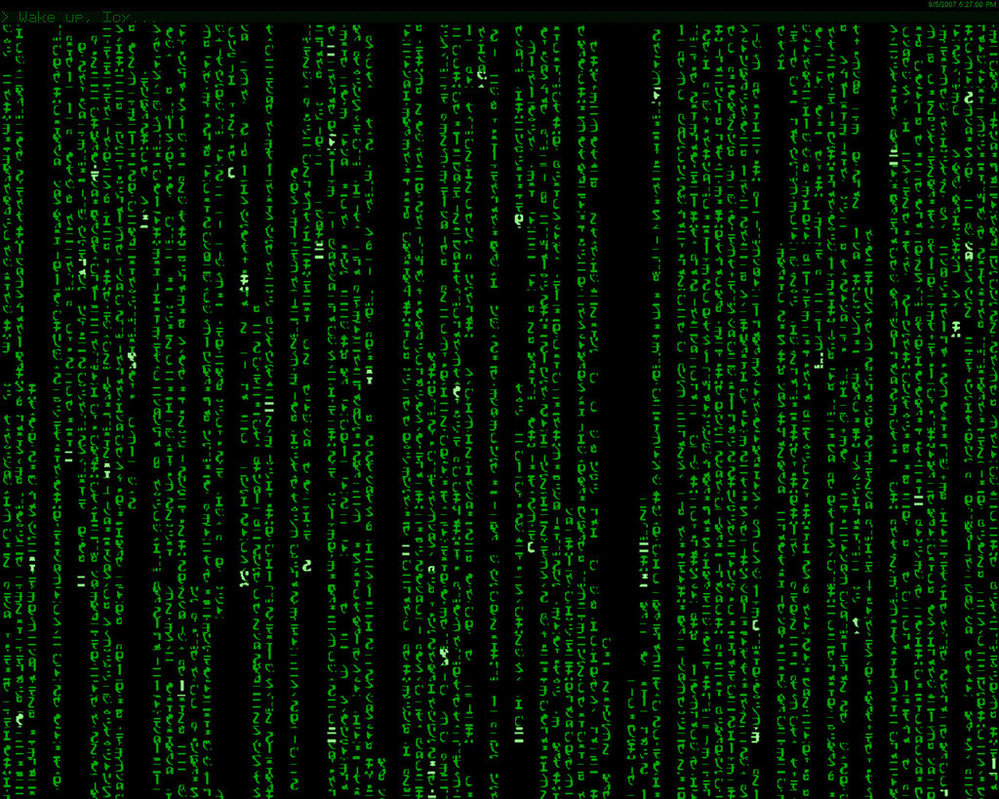
\includegraphics{./media/Data_matrix.jpg}

\hypertarget{before-starting-again}{%
\subsection*{Before Starting (again)!}\label{before-starting-again}}
\addcontentsline{toc}{subsection}{Before Starting (again)!}

Abbiamo già visto come spostare la \emph{working directory} in R Studio. Usando i comandi \texttt{getwd()} e \texttt{setwd()} ricordiamoci di selezionare la cartella relativa a questo corso. Per la lezione di oggi vediamo di organizzare la cartella del corso nel seguente modo.
La cartella, chiamata \emph{R}, deve contenere a sua volta due cartelle: \emph{data} e \emph{source}. Nella prima salveremo i dataset che ci interessano, nella seconda lo script R della lezione.

\hypertarget{pacchetti}{%
\section{Pacchetti}\label{pacchetti}}

R, come molti altri linguaggi di programmazione, ha un core di funzioni già scritte che sono disponibili all'utente, come quelle che abbiamo visto nelle lezioni precedenti. Tuttavia, con il passare del tempo, sono state sviluppate sempre più funzioni che risolvono nuovi problemi e aumentano le potenzialità di R. Tuttavia non è possibile, ne desiderabile, aggiungere tutte queste funzioni al pacchetto base di R: questo lo renderebbe più lento, occuperebbe più memoria e sarebbe pieno di funzioni che l'utente medio non userebbe!

Questa filosofia è applicata a molti altri linguaggi di programmazione che propongono un set fondamentale di funzioni accessibile a tutti (\emph{base}), e la possibilità di istallare o caricare delle estensioni per svolgere ulteriori compiti particolari.

In R queste estensioni sono i \emph{pacchetti} (package). Si può accedere alla lista dei pacchetti installati usando il comando \texttt{library()}, senza indicare argomento. Se si indica come argomento il nome di un pacchetto, R caricherà il pacchetto ed il suo contenuto sarà disponibile per l'utente.

Ad esempio, possiamo caricare il pacchetto \emph{MASS}, che ci sarà utile in seguito, con il comando \texttt{library(MASS)}.

Non tutti i pacchetti sono già installati in R, ad esempio il pacchetto \emph{hflights} non lo è.

\begin{Shaded}
\begin{Highlighting}[]
\KeywordTok{library}\NormalTok{(hflights)}
\end{Highlighting}
\end{Shaded}

Il comando da errore in quanto il pacchetto non è installato e lo possiamo installare usando il comando:

\begin{Shaded}
\begin{Highlighting}[]
\KeywordTok{install.packages}\NormalTok{(}\StringTok{'hflights'}\NormalTok{)}
\KeywordTok{library}\NormalTok{(hflights)}
\CommentTok{# ora il pacchetto viene caricato senza errori!}
\end{Highlighting}
\end{Shaded}

Alcuni pacchetti potrebbero dipendere da altri pacchetti non installati per funzionare. Per indicare a R di installare anche le dipendenze, basta inserire nel comando, dopo il nome del pacchetto l'istruzione \texttt{install.packages(\ nome\_pacchetto\ ,\ dependencies\ =\ TRUE)}.

Il comando \texttt{search()} elenca i pacchetti caricati nella sessione.

I pacchetti possono essere prodotti da qualsiasi utente e solitamente sono reperibili usando il comando indicato sopra. Di default R Studio si appoggia al sito \href{https://cran.r-project.org/}{cran} per reperire i pacchetti.

Qualora il pacchetto desiderato non fosse presente, è possibile indicare un diverso server. Ad esempio, il comando seguente permette di installare un pacchetto presente nei server di Bioconductor.

\begin{Shaded}
\begin{Highlighting}[]
\KeywordTok{source}\NormalTok{(}\StringTok{"https://bioconductor.org/biocLite.R"}\NormalTok{)}
\KeywordTok{biocLite}\NormalTok{(}\StringTok{"RnaSeqTutorial"}\NormalTok{)}
\end{Highlighting}
\end{Shaded}

Analogamente, R Studio permette di installare i pacchetti manualmente, dal menù \textbf{Tools \textbar{} Install Packages\ldots{} \textbar{} Install from: \textbar{} Package Archive File}.

L'uso del nome del pacchetto seguito da \texttt{::}, permette di accedere le funzioni e i dataset contenuti nel pacchetto. Questo è molto utile nel caso di omonimia tra funzioni. Specificando il pacchetto si può essere sicuri di usare la funzione desiderata.

\hypertarget{manipolare-dati}{%
\section{Manipolare dati}\label{manipolare-dati}}

R fornisce alcuni dataset già disponibili all'uso, mentre altri se ne possono aggiungere usando specifici pacchetti.

Ad esempio, nella lezione precedente abbiamo lavorato con il dataset \emph{mtcars} che è già disponibile. Usando i comandi precedenti abbiamo in realtà richiamato il pacchetto MASS che contiene diversi dataset e installato \emph{hflights} che contiene un altro dataset che ci tornerà utile.

\hypertarget{leggere-e-scrivere-file}{%
\subsection{Leggere e scrivere file}\label{leggere-e-scrivere-file}}

Quando si parla di dati o dataset, è possibile acquisirne in diversi modi, non solo attraverso i pacchetti. Uno dei modi più semplici e intuitivi è la lettura da file. Esistono molti formati di che possono contenere dati. I più semplici e diffusi sono i file \emph{.csv} (comma sepatated values) o i \emph{.tsv} (tab separated values).

Uno dei comandi più usati per leggere file è il comando \texttt{read.table()}. Questo permette di leggere un file e di salvarlo come data frame. Facciamo un esempio pratico.

Consideriamo il dataset \href{http://extras.springer.com/2012/978-1-4614-1301-1}{body temperature} che contiene i dati relativi alla temperatura corporea di alcuni pazienti. Salviamo il dataset nella cartella \emph{data} e leggiamolo usando la funzione \texttt{read.table()}.

\begin{Shaded}
\begin{Highlighting}[]
\NormalTok{BodyTemperature <-}\StringTok{ }\KeywordTok{read.table}\NormalTok{(}\DataTypeTok{file =} \StringTok{"./data/BodyTemperature.txt"}\NormalTok{, }\DataTypeTok{header =} \OtherTok{TRUE}\NormalTok{, }\DataTypeTok{sep =} \StringTok{" "}\NormalTok{)}
\end{Highlighting}
\end{Shaded}

La funzione read.csv accetta anche \emph{url} come argomento. In questo modo R scaricherà da solo il dataset e lo salverà nella variabile indicata.

\begin{Shaded}
\begin{Highlighting}[]
\NormalTok{BodyTemperature <-}\StringTok{ }\KeywordTok{read.csv}\NormalTok{(}\KeywordTok{url}\NormalTok{(}\StringTok{'http://extras.springer.com/2012/978-1-4614-1301-1/BodyTemperature.txt'}\NormalTok{), }\DataTypeTok{sep=}\StringTok{" "}\NormalTok{)}
\KeywordTok{head}\NormalTok{(BodyTemperature)}
\end{Highlighting}
\end{Shaded}

\begin{verbatim}
##   Gender Age HeartRate Temperature
## 1      M  33        69        97.0
## 2      M  32        72        98.8
## 3      M  42        68        96.2
## 4      F  33        75        97.8
## 5      F  26        68        98.8
## 6      M  37        79       101.3
\end{verbatim}

Gli argomenti del comando, oltre a specificare il percorso in cui si trova il file da leggere, indicano che sono presenti degli \emph{header}, cioè intestazioni che riportano il nome delle variabili, e che il separatore usato nel file per indicare i diversi elementi delle righe è lo spazio. Lo spazio è il separatore di default di \texttt{read.table()} ma è possibile indicarne di diversi. Se il file fosse stato un csv (\emph{comma separated values}) avremmo indicato \texttt{sep=","}. Allo stesso modo avremmo potuto usare la funzione \texttt{read.csv()} che considera la virgola come separatore di default. Se i valori fossero stati separati da punto e virgola avremmo potuto usare \texttt{read.csv2()} e \texttt{read.delim()} se separate da tab (\t).

In modo del tutto simile, la funzione \texttt{write.table()} permette di scrivere un data frame (o una variabile) in un file. Ad esempio, il comando seguente scrive il dataset scaricato da internet nella cartella data come file csv.

\begin{Shaded}
\begin{Highlighting}[]
\KeywordTok{write.csv}\NormalTok{(BodyTemperature, }\StringTok{"./data/BodyTemperature.txt"}\NormalTok{)}
\end{Highlighting}
\end{Shaded}

\hypertarget{esplorare-i-file}{%
\subsection{Esplorare i file}\label{esplorare-i-file}}

Una volta letto o caricato il dataset che ci interessa è ora di iniziare ad analizzare i \href{http://phdcomics.com/comics.php?f=1816}{dati} che contiene. Spesso i dataset sono accompagnati da delle descrizioni che ne spiegano il contenuto ed è buona regola leggerle.

Possiamo visualizzare la testa del dataset o la coda, usando i comandi \texttt{head()} e \texttt{tail()} o anche visualizzare l'intero dataset in una finestra di R Studio usando il comando \texttt{View()}. Possiamo conoscerne le dimensioni con la funzione \texttt{dim()} e possiamo conoscere i nomi delle colonne con la funzione \texttt{names()}.
\texttt{str()} restituisce invece informazioni sulla struttura del dataset. In R Studio, l'equivalente di questo comando è accessibile nella finesta \textbf{Environment}. L'uso di queste funzioni è sempre utile per iniziare a capire i dati con cui si ha a che fare.

Una funzione utilissima è \texttt{summary()}. Questa restituisce diverse informazioni per le \emph{variabili numeriche}: minimo, massimo, media e i quartili. Va specificato \emph{numeriche} in quanto un data frame potrebbe anche contenere delle variabili non numeriche. Nel caso di BodyTemperature ad esempio, la prima colonna è la variabile categorica del sesso del paziente.

Altre funzione utili sono le funzioni come \texttt{mean()} e \texttt{sd()} che ci restituiscono media e standard deviation dell'argomento passato.
Le funzioni \texttt{IQR()} e \texttt{range()} restituiscono la distanza interquartile ed il range.

Un utile comando per applicare funzioni pensate per elementi scalari agli elementi di un array o una matrice è la funzione \texttt{apply()}. Tale funzione è utile anche per applicare funzioni lungo una sola dimensione. Le varianti \texttt{lapply()} e \texttt{tapply()} funzionano in modo simile. Un altro comando per la manipolazione di dati è \texttt{round()} che arrotonda un valore o un vettore all'intero più vicino, o indicando il numero di cifre decimali, arrotonda fino alle cifre decimali indicati.

Altre funzioni utili sono \texttt{sort()}, che ordina gli elementi di un vettore, \texttt{unique()} che rimuove le entrate ripetute da array o data frame. Le funzioni come \texttt{any()} e \texttt{which()} verificano se una condizione è soddisfatta. La prima restituisce \texttt{TRUE} se almeno un elemento che verifica la condizione, mentre \texttt{which()} che riporta l'indice degli elementi che la soddisfano.

Vediamo alcuni esempi con il dataset \texttt{BodyTemperature}.

\hypertarget{factors}{%
\subsection{Factors}\label{factors}}

A volte alcune variabili categoriche sono salvate come variabili numeriche. Esploriamo ad esempio il dataset \emph{birthwt} (birth weight) contenuto nel pacchetto MASS. Possiamo notare che alcune variabili, sebbene siano numeriche, rappresentano delle categorie: ad esempio fumatori o no, o ipertesi o no. Tuttavia, se usiamo il comando \texttt{summary()}, vediamo che vengono trattate come variabili numeriche. Il comando \texttt{as.factor()} permette di convertire variabili numeriche in variabili categoriche.

\begin{Shaded}
\begin{Highlighting}[]
\KeywordTok{library}\NormalTok{(MASS)}
\NormalTok{birthwt1 <-}\StringTok{ }\NormalTok{birthwt}
\NormalTok{birthwt1}\OperatorTok{$}\NormalTok{race <-}\StringTok{ }\KeywordTok{as.factor}\NormalTok{(birthwt1}\OperatorTok{$}\NormalTok{race)}
\end{Highlighting}
\end{Shaded}

Dalla descrizione delle variabili fornita da R Studio nella finestra \textbf{Environment}, possiamo vedere che dopo l'assegnazione, race è indicato come factor, non più integer.

La funzione \texttt{table()} costruisce una contingency table tra le combinazioni di factors mentre \texttt{levels()} restituisce gli attributi di livello di una variabile. Usando \texttt{levels()} è anche possibile assegnare o variare gli attributi di livello.

\hypertarget{missing-data}{%
\section{Missing data}\label{missing-data}}

Spesso i dati forniti contengono valori non affidabili, oppure ci sono errori in qualche riga o ancora mancano dei valori. Questo è un grande problema, sia perché, se non riconosciuti in anticipo, questi valori possono influenzare i nostri risultati, sia perché non esistono protocolli standard per affrontare questi casi.

Alcuni elementi posso non essere stati inseriti ed essi solitamente vengono segnalati con NA (not available). R ha una funzione dedicata per trovare questi elementi: \texttt{is.na()}. Tale funzione restituisce valori booleani per indicare se il contenuto è NA o no. Analogamente, \texttt{na.omit()} restituisce l'argomento privato delle righe contenenti NA.

In modo del tutto analogo funziona il comando \texttt{is.nan()} che però verifica se il contenuto è NaN (not a number). Esistono anche i controlli \texttt{is.infinite()} e \texttt{is.finite()} che verificano se ci sono valori \texttt{Inf/-Inf}.

\hypertarget{manipolare-i-dati}{%
\section{Manipolare i dati}\label{manipolare-i-dati}}

Abbiamo ampiamente visto come lavorare e manipolare i dati. Tuttavia un importante funzione che permette di raggruppare i dati non è stata spiegata in classe: si tratta di \texttt{aggregate()}. Tale comando, permette di applicare una funzione ad un sottoinsieme dei dati, seguendo uno schema preciso. Vediamo alcuni esempi.

Altro utile comando è \texttt{merge()} che permette di unire dataframe indicando il campo da usare per confrontare le entrate. In modo più semplice, e dopo essersi assicurati che le osservazioni siano ``allineate'', è possibile usare anche i comandi \texttt{rbin()} e \texttt{cbind()} che sono già stati trattati.

\hypertarget{distribuzioni-di-probabilita}{%
\section{Distribuzioni di probabilità}\label{distribuzioni-di-probabilita}}

R ci permette di accedere a molte distribuzioni di probabilità attraverso delle apposite funzioni che sono contenuto nel pacchetto \emph{stast}, che va quindi caricato.

Le distribuzioni sono accessibili attraverso delle funzioni che richiamano il nome della distribuzione, ad esempio con \emph{norm}, \emph{binom} e \emph{gamma}, solo per citarne alcune, si accede alla distribuzione normale, binomiale e gamma. A tale nome si aggiunge un \emph{prefisso}, che serve a specificare se si è interessati alla funzione densità (\emph{d}), alla distribuzione (\emph{p}), alla funzione che riporta i quantili (\emph{q}) o se si vogliono generare dei numeri usando tale distribuzione (\emph{r}).

Cercando \emph{distribution} nell'help è possibile accedere all'elenco di tutte le distribuzioni di R. Il fatto che R permetta di accedere facilmente alle distribuzioni tornerà particolarmente utile quando lavoreremo con gli intervalli di confidenza, e potremmo interrogare R, piuttosto che lavorare con la versione tabulare delle stesse.

Va segnalata, almeno per la distribuzione normale, che esiste la funzione \texttt{qqnorm} che permette di confrontare graficamente i quantili dei propri dati con quelli della distribuzione normale. Questo è un modo per verificare graficamente (e quindi non formalmente) se i propri dati seguono una distribuzione normale. Insieme alla richiesta che le misurazioni siano indipendenti, queste due sono delle ipotesi che abbiamo visto molto spesso, specialmente nell'uso di teoremi limite.

\hypertarget{visualizzare-i-dati}{%
\chapter{Visualizzare i dati}\label{visualizzare-i-dati}}

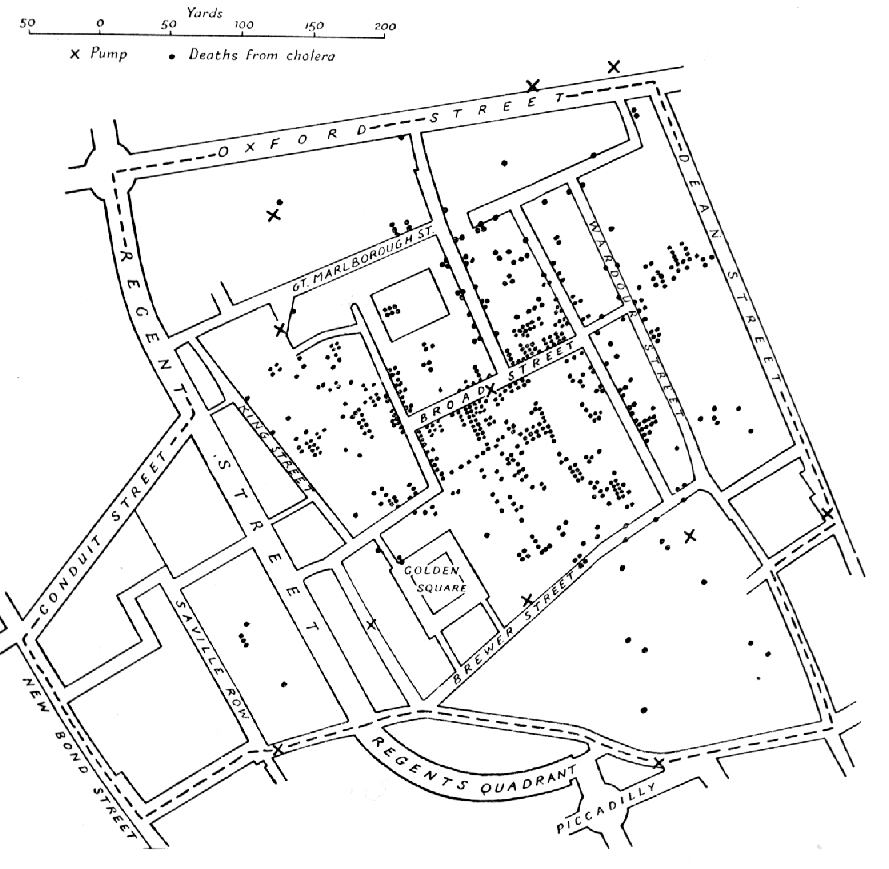
\includegraphics{./media/Cholera.jpg}
This \href{https://it.wikipedia.org/wiki/John_Snow_(medico)}{John Snow} knew something!

La visualizzazione dei dati permettere di individuare trend, connessioni e carpire informazioni dai dati che in forma tabulare non sono ovvie.

I comandi che seguono aiutano in tali indagini. Tutti questi comandi possono essere personalizzati usando diversi colori, personalizzando le label degli assi o affiancando le immagini.

Un pacchetto che permette non solo di produrre immagini (un po' più belle), ma anche di utilizzare funzioni avanzate è \href{http://ggplot2.org/}{ggplot2} che però non tratteremo in questo corso.

Oltre ad introdurre alcune funzioni che permettono di ottenere dei grafici, esploreremo anche alcuni dataset.

\hypertarget{box-plot}{%
\section{Box plot}\label{box-plot}}

A lezione abbiamo già incontrato i boxplot. Usando R è molto semplice produrre dei boxplot usando gli appositi comandi. Vediamoli usando il dataset \emph{birthwt}, contenuto in MASS.

\begin{Shaded}
\begin{Highlighting}[]
\KeywordTok{library}\NormalTok{(MASS)}
\KeywordTok{boxplot}\NormalTok{(birthwt}\OperatorTok{$}\NormalTok{bwt)}
\end{Highlighting}
\end{Shaded}

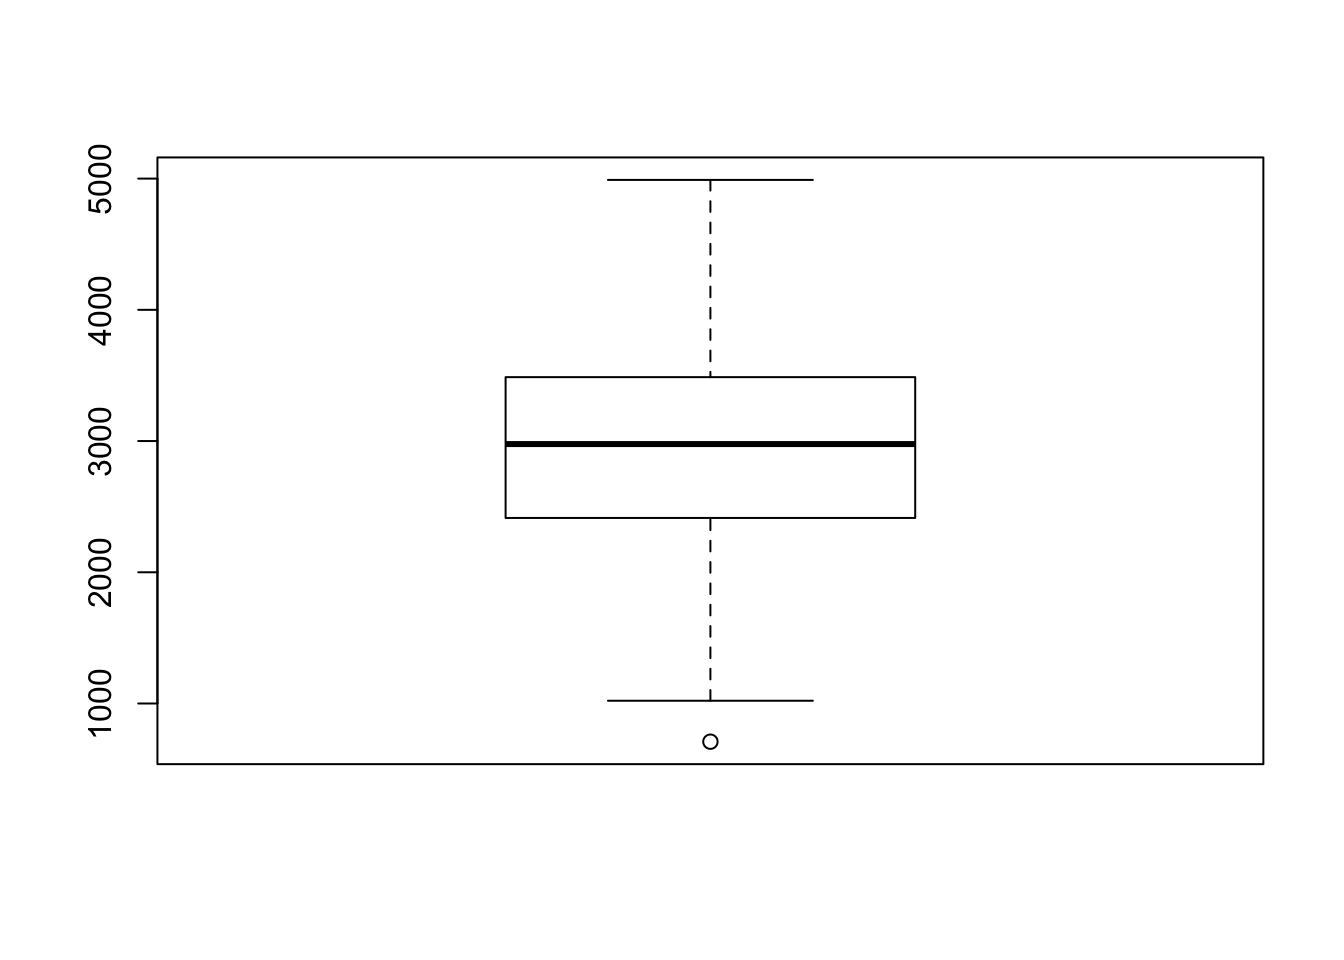
\includegraphics{bookdown_files/figure-latex/unnamed-chunk-37-1.pdf}

La seguente notazione permette di produrre più boxplot relativi a bwt, divisi rispetto alla variabile race.

\begin{Shaded}
\begin{Highlighting}[]
\KeywordTok{boxplot}\NormalTok{(bwt }\OperatorTok{~}\StringTok{ }\NormalTok{race, }\DataTypeTok{data =}\NormalTok{ birthwt )}
\end{Highlighting}
\end{Shaded}

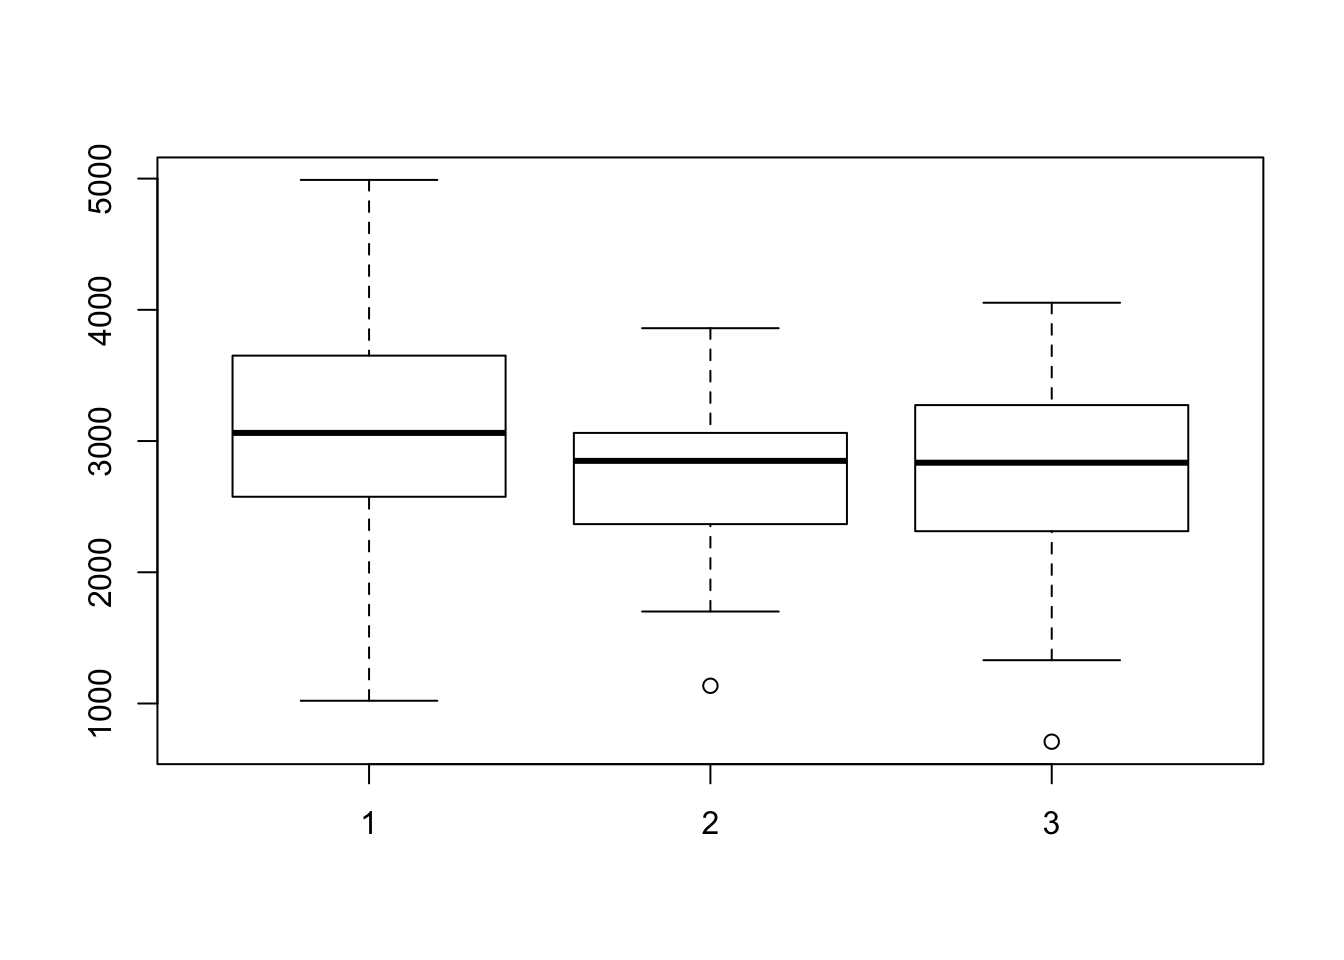
\includegraphics{bookdown_files/figure-latex/unnamed-chunk-38-1.pdf}

\emph{Esercizio}
Si investighi la variabile lwt rispetto a race e smoke.

\emph{Esercizio}
Si noti che il pacchetto \emph{car} contiene una funzione chiamata \texttt{Boxplot()}, con la maiuscola, che vicino ai potenziali outliers indica l'indice dell'elemento. Si replichino i precedenti boxplot usando tale funzione.

\hypertarget{istogrammi-e-scatter-plost}{%
\section{Istogrammi e scatter plost}\label{istogrammi-e-scatter-plost}}

Usando il comando \texttt{hist()} è possibile ottenere degli istogrammi per le variabili, passando gli argomenti in modo analogo ai boxplot.

Analogamente, con i comandi \texttt{plot(x,y)} or \texttt{scatterplot(x,y)} è possibile rappresentare i dati come punti.

Vedremo che questo può essere molto utile per ottenere degli indizi sulle relazioni tra variabili.

\hypertarget{analizzare-il-dataset-body-temperature}{%
\section{Analizzare il dataset Body Temperature}\label{analizzare-il-dataset-body-temperature}}

BodyTemperature è un dataset che contiene la misurazione di quattro variabili (sesso, età, frequenza cardiaca e temperatura corporea ascellare) di 100 pazienti. Possiamo leggere importare il file specificando invece che il percorso, l'indirizzo url.

\begin{Shaded}
\begin{Highlighting}[]
\NormalTok{BodyTemperature <-}\StringTok{ }\KeywordTok{read.csv}\NormalTok{(}\KeywordTok{url}\NormalTok{(}\StringTok{'http://extras.springer.com/2012/978-1-4614-1301-1/BodyTemperature.txt'}\NormalTok{))}
\end{Highlighting}
\end{Shaded}

Se però visualizziamo questo dataset qualosa non torna.
Il comando giusto specifica quale separatore viene considerato: in questo caso lo spazio, che è diverso da quello di default di \texttt{read.csv}. In modo analogo avremmo potuto leggere i dati usando \texttt{read.table()}. Tuttavia, controllaimo bene l'output per capire se effettivamente il dataset è stato letto nel modo giusto!

\begin{Shaded}
\begin{Highlighting}[]
\NormalTok{BodyTemperature <-}\StringTok{ }\KeywordTok{read.table}\NormalTok{(}\KeywordTok{url}\NormalTok{(}\StringTok{'http://extras.springer.com/2012/978-1-4614-1301-1/BodyTemperature.txt'}\NormalTok{))}
\end{Highlighting}
\end{Shaded}

\begin{Shaded}
\begin{Highlighting}[]
\NormalTok{BodyTemperature <-}\StringTok{ }\KeywordTok{read.csv}\NormalTok{(}\KeywordTok{url}\NormalTok{(}\StringTok{'http://extras.springer.com/2012/978-1-4614-1301-1/BodyTemperature.txt'}\NormalTok{), }\DataTypeTok{sep=} \StringTok{" "}\NormalTok{)}
\end{Highlighting}
\end{Shaded}

Esploriamo un po' il dataset per capirne il contenuto e le variabili

\begin{Shaded}
\begin{Highlighting}[]
\KeywordTok{str}\NormalTok{(BodyTemperature)}
\end{Highlighting}
\end{Shaded}

\begin{verbatim}
## 'data.frame':    100 obs. of  4 variables:
##  $ Gender     : Factor w/ 2 levels "F","M": 2 2 2 1 1 2 1 1 1 2 ...
##  $ Age        : int  33 32 42 33 26 37 32 45 31 49 ...
##  $ HeartRate  : int  69 72 68 75 68 79 71 73 77 81 ...
##  $ Temperature: num  97 98.8 96.2 97.8 98.8 ...
\end{verbatim}

\begin{Shaded}
\begin{Highlighting}[]
\KeywordTok{head}\NormalTok{(BodyTemperature)}
\end{Highlighting}
\end{Shaded}

\begin{verbatim}
##   Gender Age HeartRate Temperature
## 1      M  33        69        97.0
## 2      M  32        72        98.8
## 3      M  42        68        96.2
## 4      F  33        75        97.8
## 5      F  26        68        98.8
## 6      M  37        79       101.3
\end{verbatim}

\begin{Shaded}
\begin{Highlighting}[]
\KeywordTok{names}\NormalTok{(BodyTemperature)}
\end{Highlighting}
\end{Shaded}

\begin{verbatim}
## [1] "Gender"      "Age"         "HeartRate"   "Temperature"
\end{verbatim}

Solo a scopo didattico, vediamo l'applicazione di uno dei comandi visti: \texttt{levels()}:

\begin{Shaded}
\begin{Highlighting}[]
\NormalTok{BodyTemperature}\OperatorTok{$}\NormalTok{GenderLong <-}\StringTok{ }\NormalTok{BodyTemperature}\OperatorTok{$}\NormalTok{Gender}
\KeywordTok{levels}\NormalTok{(BodyTemperature}\OperatorTok{$}\NormalTok{GenderLong) <-}\StringTok{ }\KeywordTok{c}\NormalTok{(}\StringTok{"Female"}\NormalTok{, }\StringTok{"Male"}\NormalTok{)}
\end{Highlighting}
\end{Shaded}

\begin{Shaded}
\begin{Highlighting}[]
\KeywordTok{summary}\NormalTok{(BodyTemperature)}
\end{Highlighting}
\end{Shaded}

\begin{verbatim}
##  Gender      Age          HeartRate      Temperature    
##  F:51   Min.   :21.00   Min.   :61.00   Min.   : 96.20  
##  M:49   1st Qu.:33.75   1st Qu.:69.00   1st Qu.: 97.70  
##         Median :37.00   Median :73.00   Median : 98.30  
##         Mean   :37.62   Mean   :73.66   Mean   : 98.33  
##         3rd Qu.:42.00   3rd Qu.:78.00   3rd Qu.: 98.90  
##         Max.   :50.00   Max.   :87.00   Max.   :101.30
\end{verbatim}

\begin{Shaded}
\begin{Highlighting}[]
\KeywordTok{range}\NormalTok{(BodyTemperature[,}\OperatorTok{-}\DecValTok{1}\NormalTok{])}
\end{Highlighting}
\end{Shaded}

\begin{verbatim}
## [1]  21.0 101.3
\end{verbatim}

In modo analogo possiamo cercare di ottenere la distanza interquartile per i gli elementi del dataset con \texttt{IQR(BodyTemperature{[},2:4{]})}, tuttavia questo ci da errore.

Possiamo aggirare questa limitazione usando il comando \texttt{apply()}. La stessa funzione la possiamo usare per individuare, ad esempio, il valore minimo rispetto alle variabili (numeriche) e quale indice lo assume.

\begin{Shaded}
\begin{Highlighting}[]
\KeywordTok{apply}\NormalTok{(BodyTemperature[,}\OperatorTok{-}\DecValTok{1}\NormalTok{], }\DecValTok{2}\NormalTok{, IQR )}
\end{Highlighting}
\end{Shaded}

\begin{verbatim}
##         Age   HeartRate Temperature 
##        8.25        9.00        1.20
\end{verbatim}

\begin{Shaded}
\begin{Highlighting}[]
\KeywordTok{apply}\NormalTok{(BodyTemperature[,}\OperatorTok{-}\DecValTok{1}\NormalTok{], }\DecValTok{2}\NormalTok{, min )}
\end{Highlighting}
\end{Shaded}

\begin{verbatim}
##         Age   HeartRate Temperature 
##        21.0        61.0        96.2
\end{verbatim}

\begin{Shaded}
\begin{Highlighting}[]
\KeywordTok{apply}\NormalTok{(BodyTemperature[,}\OperatorTok{-}\DecValTok{1}\NormalTok{], }\DecValTok{2}\NormalTok{, which.min )}
\end{Highlighting}
\end{Shaded}

\begin{verbatim}
##         Age   HeartRate Temperature 
##          37          28           3
\end{verbatim}

Possiamo notare che la temperatura non è espressa in gradi Celsius (°C), bensì in Fahrenheit (F). Usando delle semplici operazioni di base possiamo trasformare le temperature in gradi Celsius e salvare questi nuovi dati nella colonna che chiamiamo \emph{TempC}.

\begin{Shaded}
\begin{Highlighting}[]
\NormalTok{fromFtoC <-}\StringTok{ }\ControlFlowTok{function}\NormalTok{(dataF) \{}
\KeywordTok{return}\NormalTok{((dataF }\OperatorTok{-}\StringTok{ }\DecValTok{32}\NormalTok{)}\OperatorTok{*}\NormalTok{(}\DecValTok{5}\OperatorTok{/}\DecValTok{9}\NormalTok{)) }
\NormalTok{\}}
\NormalTok{BodyTemperature}\OperatorTok{$}\NormalTok{TempC <-}\StringTok{ }\NormalTok{(BodyTemperature}\OperatorTok{$}\NormalTok{Temperature }\DecValTok{-32}\NormalTok{)}\OperatorTok{*}\DecValTok{5}\OperatorTok{/}\DecValTok{9}

\KeywordTok{head}\NormalTok{(BodyTemperature)}
\end{Highlighting}
\end{Shaded}

\begin{verbatim}
##   Gender Age HeartRate Temperature    TempC
## 1      M  33        69        97.0 36.11111
## 2      M  32        72        98.8 37.11111
## 3      M  42        68        96.2 35.66667
## 4      F  33        75        97.8 36.55556
## 5      F  26        68        98.8 37.11111
## 6      M  37        79       101.3 38.50000
\end{verbatim}

\hypertarget{visualizzare-il-dataset-bodytemperature}{%
\section{Visualizzare il dataset BodyTemperature}\label{visualizzare-il-dataset-bodytemperature}}

Passiamo ora a visualizzare il contenuto del dateset.

\begin{Shaded}
\begin{Highlighting}[]
\KeywordTok{hist}\NormalTok{(BodyTemperature}\OperatorTok{$}\NormalTok{TempC )}
\end{Highlighting}
\end{Shaded}

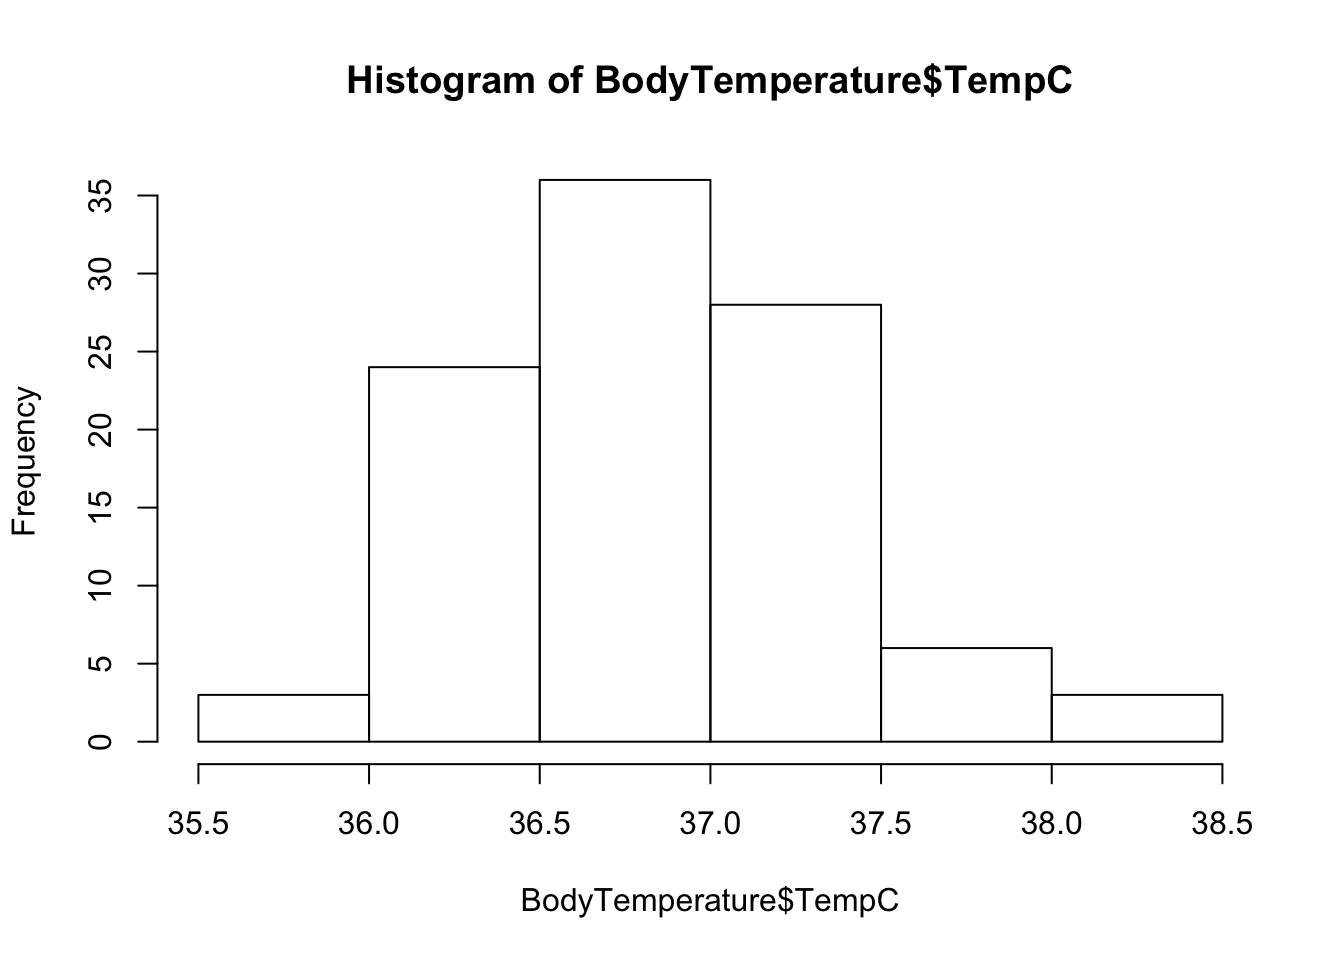
\includegraphics{bookdown_files/figure-latex/unnamed-chunk-48-1.pdf}

\begin{Shaded}
\begin{Highlighting}[]
\KeywordTok{boxplot}\NormalTok{(TempC }\OperatorTok{~}\StringTok{ }\NormalTok{Gender, }\DataTypeTok{data =}\NormalTok{ BodyTemperature)}
\end{Highlighting}
\end{Shaded}

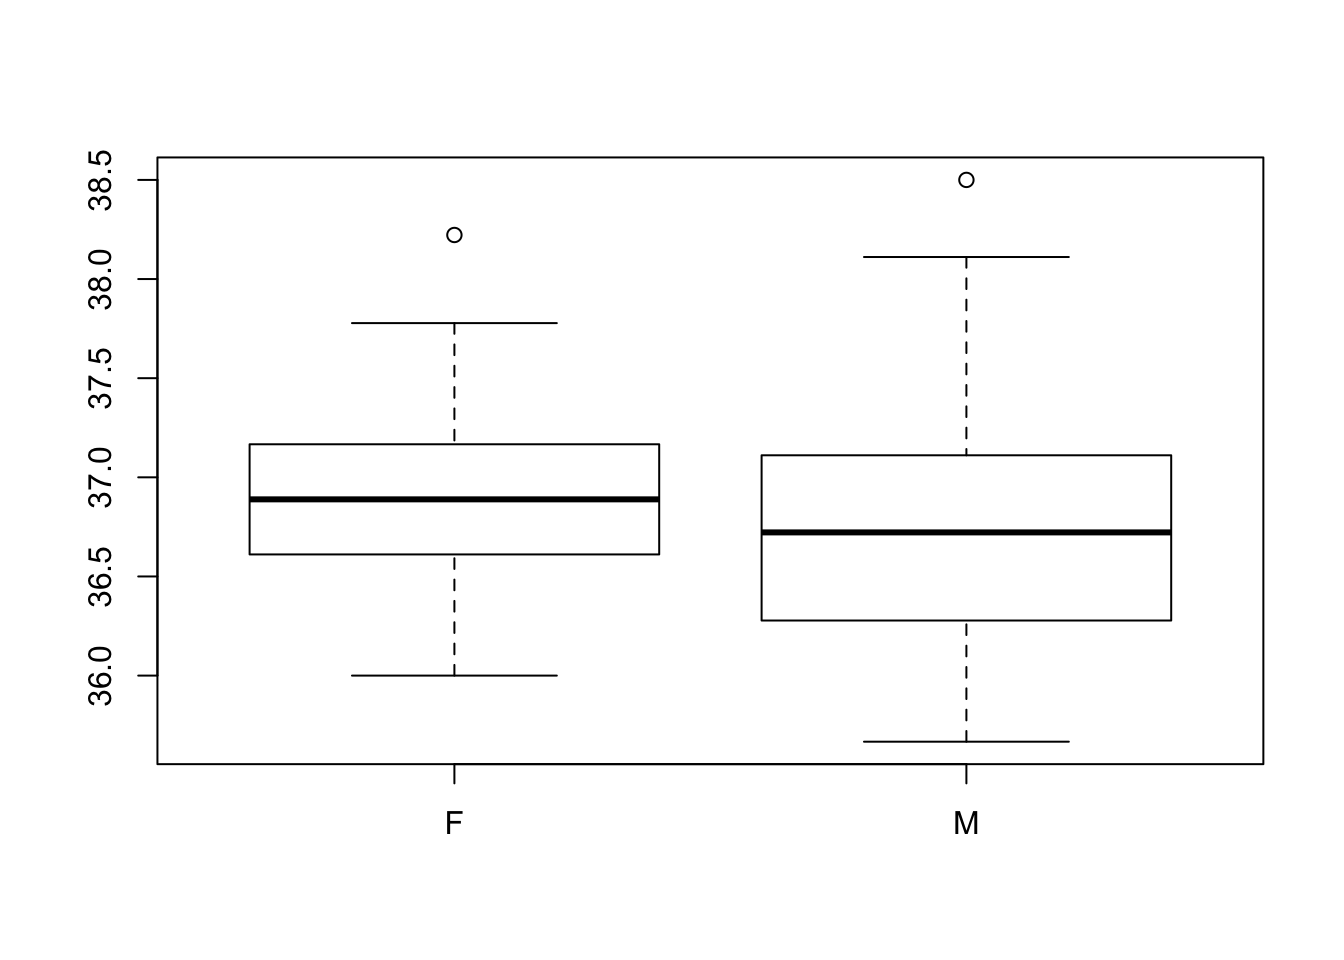
\includegraphics{bookdown_files/figure-latex/unnamed-chunk-49-1.pdf}

Vediamo ora come affiancare diversi plot e usiamo alcuni dei parametri delle funzioni di plot.

\begin{Shaded}
\begin{Highlighting}[]
\KeywordTok{par}\NormalTok{(}\DataTypeTok{mfrow=}\KeywordTok{c}\NormalTok{(}\DecValTok{1}\NormalTok{, }\DecValTok{2}\NormalTok{))}
\KeywordTok{hist}\NormalTok{(BodyTemperature}\OperatorTok{$}\NormalTok{TempC, }\DataTypeTok{main =} \StringTok{""}\NormalTok{, }\DataTypeTok{xlab =} \StringTok{"°C"}\NormalTok{)}
\KeywordTok{boxplot}\NormalTok{(TempC }\OperatorTok{~}\StringTok{ }\NormalTok{Gender, }\DataTypeTok{data =}\NormalTok{ BodyTemperature, }\DataTypeTok{xlab =} \StringTok{"Gender"}\NormalTok{, }\DataTypeTok{ylab =} \StringTok{"Temperature [°C]"}\NormalTok{)}
\end{Highlighting}
\end{Shaded}

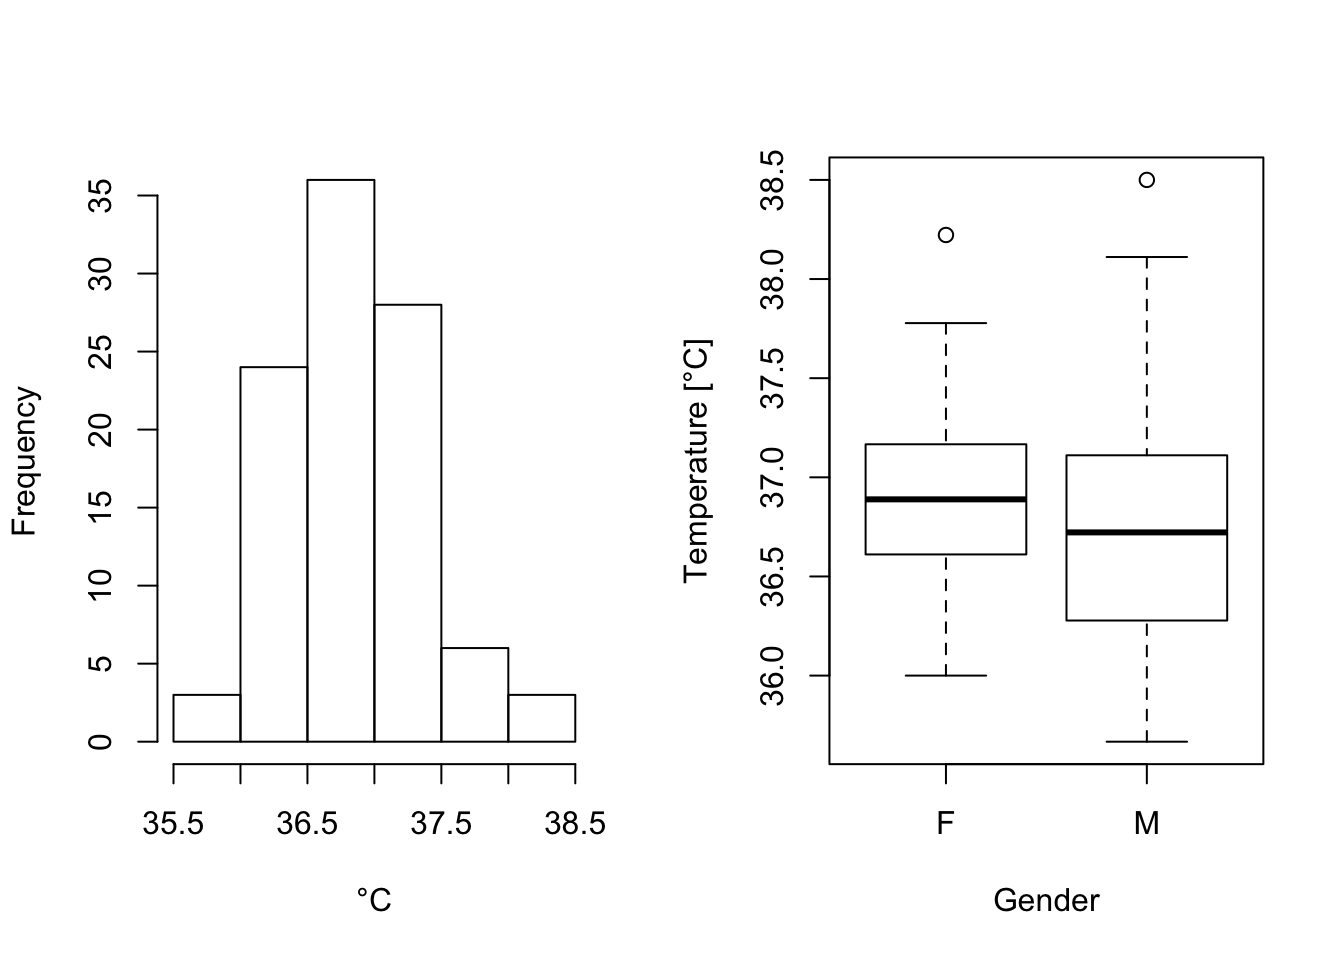
\includegraphics{bookdown_files/figure-latex/unnamed-chunk-50-1.pdf}

\begin{Shaded}
\begin{Highlighting}[]
\KeywordTok{par}\NormalTok{(}\DataTypeTok{mfrow=}\KeywordTok{c}\NormalTok{(}\DecValTok{1}\NormalTok{, }\DecValTok{2}\NormalTok{))}
\KeywordTok{boxplot}\NormalTok{(BodyTemperature}\OperatorTok{$}\NormalTok{TempC , }\DataTypeTok{ylab =} \StringTok{"Temperature [°C]"}\NormalTok{)}
\KeywordTok{boxplot}\NormalTok{(TempC }\OperatorTok{~}\StringTok{ }\NormalTok{Gender, }\DataTypeTok{data =}\NormalTok{ BodyTemperature, }\DataTypeTok{xlab =} \StringTok{"Gender"}\NormalTok{)}
\end{Highlighting}
\end{Shaded}

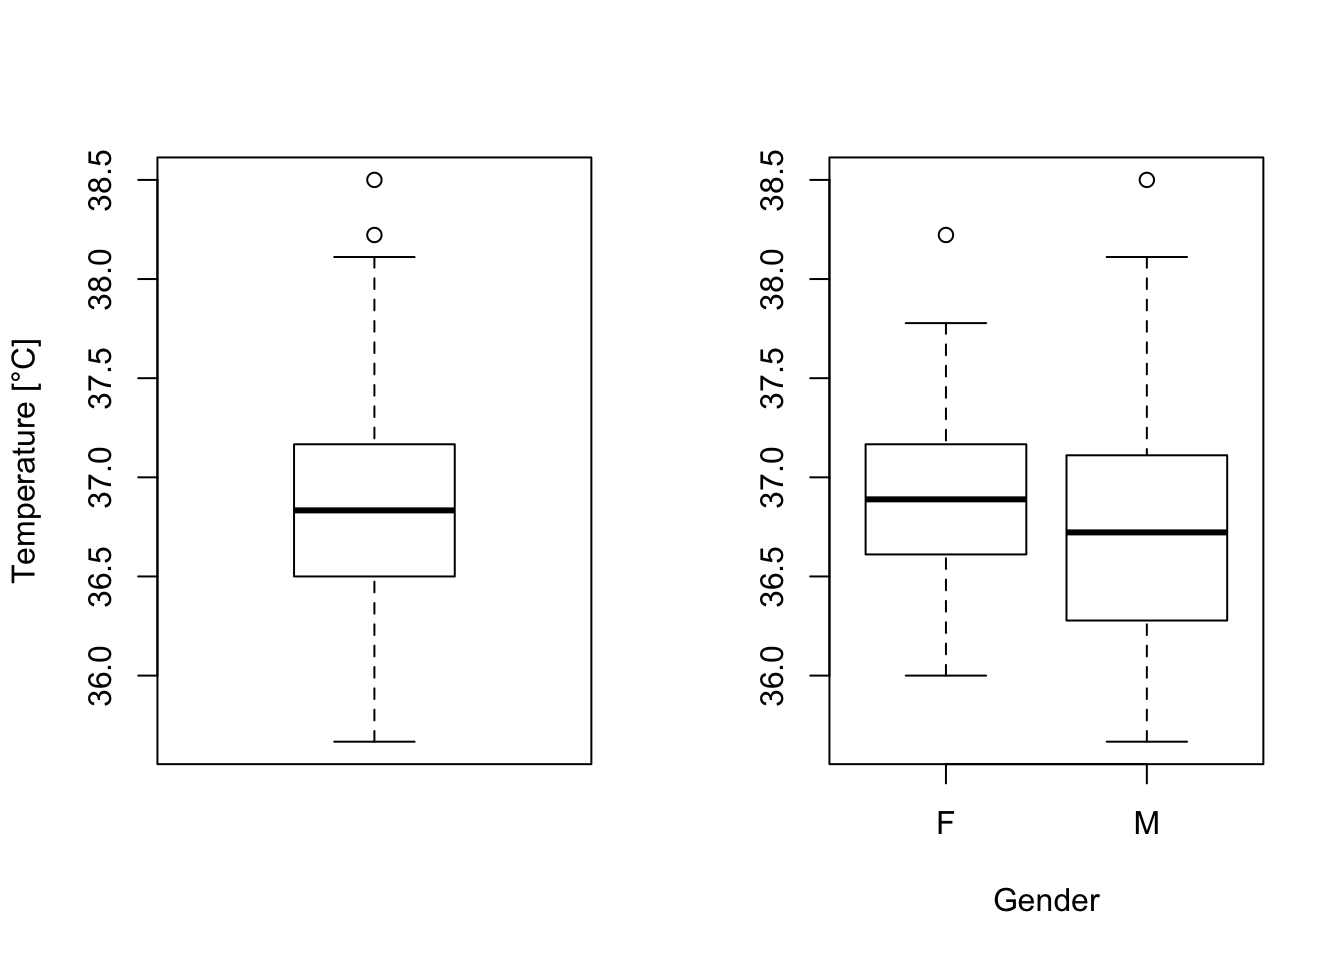
\includegraphics{bookdown_files/figure-latex/unnamed-chunk-51-1.pdf}

\begin{Shaded}
\begin{Highlighting}[]
\KeywordTok{par}\NormalTok{(}\DataTypeTok{mfrow=}\KeywordTok{c}\NormalTok{(}\DecValTok{1}\NormalTok{, }\DecValTok{2}\NormalTok{))}
\KeywordTok{boxplot}\NormalTok{(BodyTemperature}\OperatorTok{$}\NormalTok{TempC , }\DataTypeTok{ylab =} \StringTok{"Temperature [°C]"}\NormalTok{)}
\KeywordTok{boxplot}\NormalTok{(TempC }\OperatorTok{~}\StringTok{ }\NormalTok{Gender, }\DataTypeTok{data =}\NormalTok{ BodyTemperature, }\DataTypeTok{xlab =} \StringTok{"Gender"}\NormalTok{)}
\KeywordTok{title}\NormalTok{(}\StringTok{"Boxplots for Temperature"}\NormalTok{, }\DataTypeTok{outer =}\NormalTok{ T, }\DataTypeTok{line =} \DecValTok{-2}\NormalTok{)}
\end{Highlighting}
\end{Shaded}

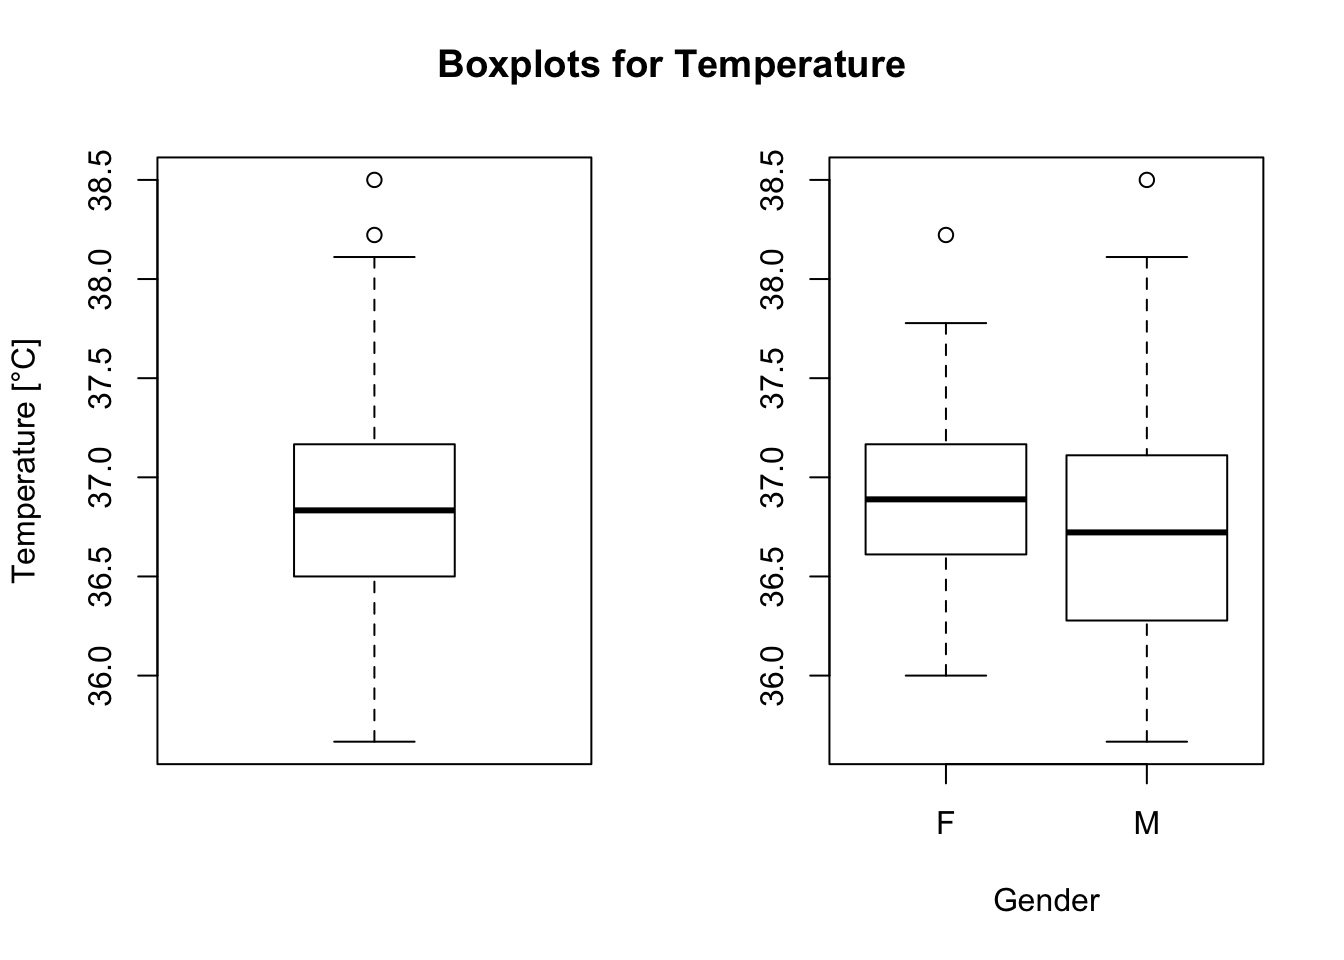
\includegraphics{bookdown_files/figure-latex/unnamed-chunk-52-1.pdf}

\begin{Shaded}
\begin{Highlighting}[]
\KeywordTok{par}\NormalTok{(}\DataTypeTok{mfrow=}\KeywordTok{c}\NormalTok{(}\DecValTok{2}\NormalTok{, }\DecValTok{2}\NormalTok{))}
\KeywordTok{hist}\NormalTok{((BodyTemperature}\OperatorTok{$}\NormalTok{TempC) , }\DataTypeTok{xlab =} \StringTok{"Temperature [°C]"}\NormalTok{, }\DataTypeTok{main =} \StringTok{""}\NormalTok{)}
\KeywordTok{boxplot}\NormalTok{(TempC }\OperatorTok{~}\StringTok{ }\NormalTok{Gender, }\DataTypeTok{data =}\NormalTok{ BodyTemperature, }\DataTypeTok{xlab =} \StringTok{"Gender"}\NormalTok{)}
\KeywordTok{hist}\NormalTok{(BodyTemperature}\OperatorTok{$}\NormalTok{TempC[BodyTemperature}\OperatorTok{$}\NormalTok{Gender }\OperatorTok{==}\StringTok{ "F"}\NormalTok{],}\DataTypeTok{freq =} \OtherTok{FALSE}\NormalTok{ ,}\DataTypeTok{main =} \StringTok{"Female"}\NormalTok{, }\DataTypeTok{col =} \StringTok{"pink"}\NormalTok{, }\DataTypeTok{xlab =} \StringTok{"Temperature [°C]"}\NormalTok{)}
\KeywordTok{hist}\NormalTok{(BodyTemperature}\OperatorTok{$}\NormalTok{TempC[BodyTemperature}\OperatorTok{$}\NormalTok{Gender }\OperatorTok{==}\StringTok{ "M"}\NormalTok{],}\DataTypeTok{freq =} \OtherTok{FALSE}\NormalTok{ ,}\DataTypeTok{main =} \StringTok{"Male"}\NormalTok{, }\DataTypeTok{col =} \StringTok{"skyblue"}\NormalTok{ , }\DataTypeTok{xlab =} \StringTok{"Temperature [°C]"}\NormalTok{)}
\end{Highlighting}
\end{Shaded}

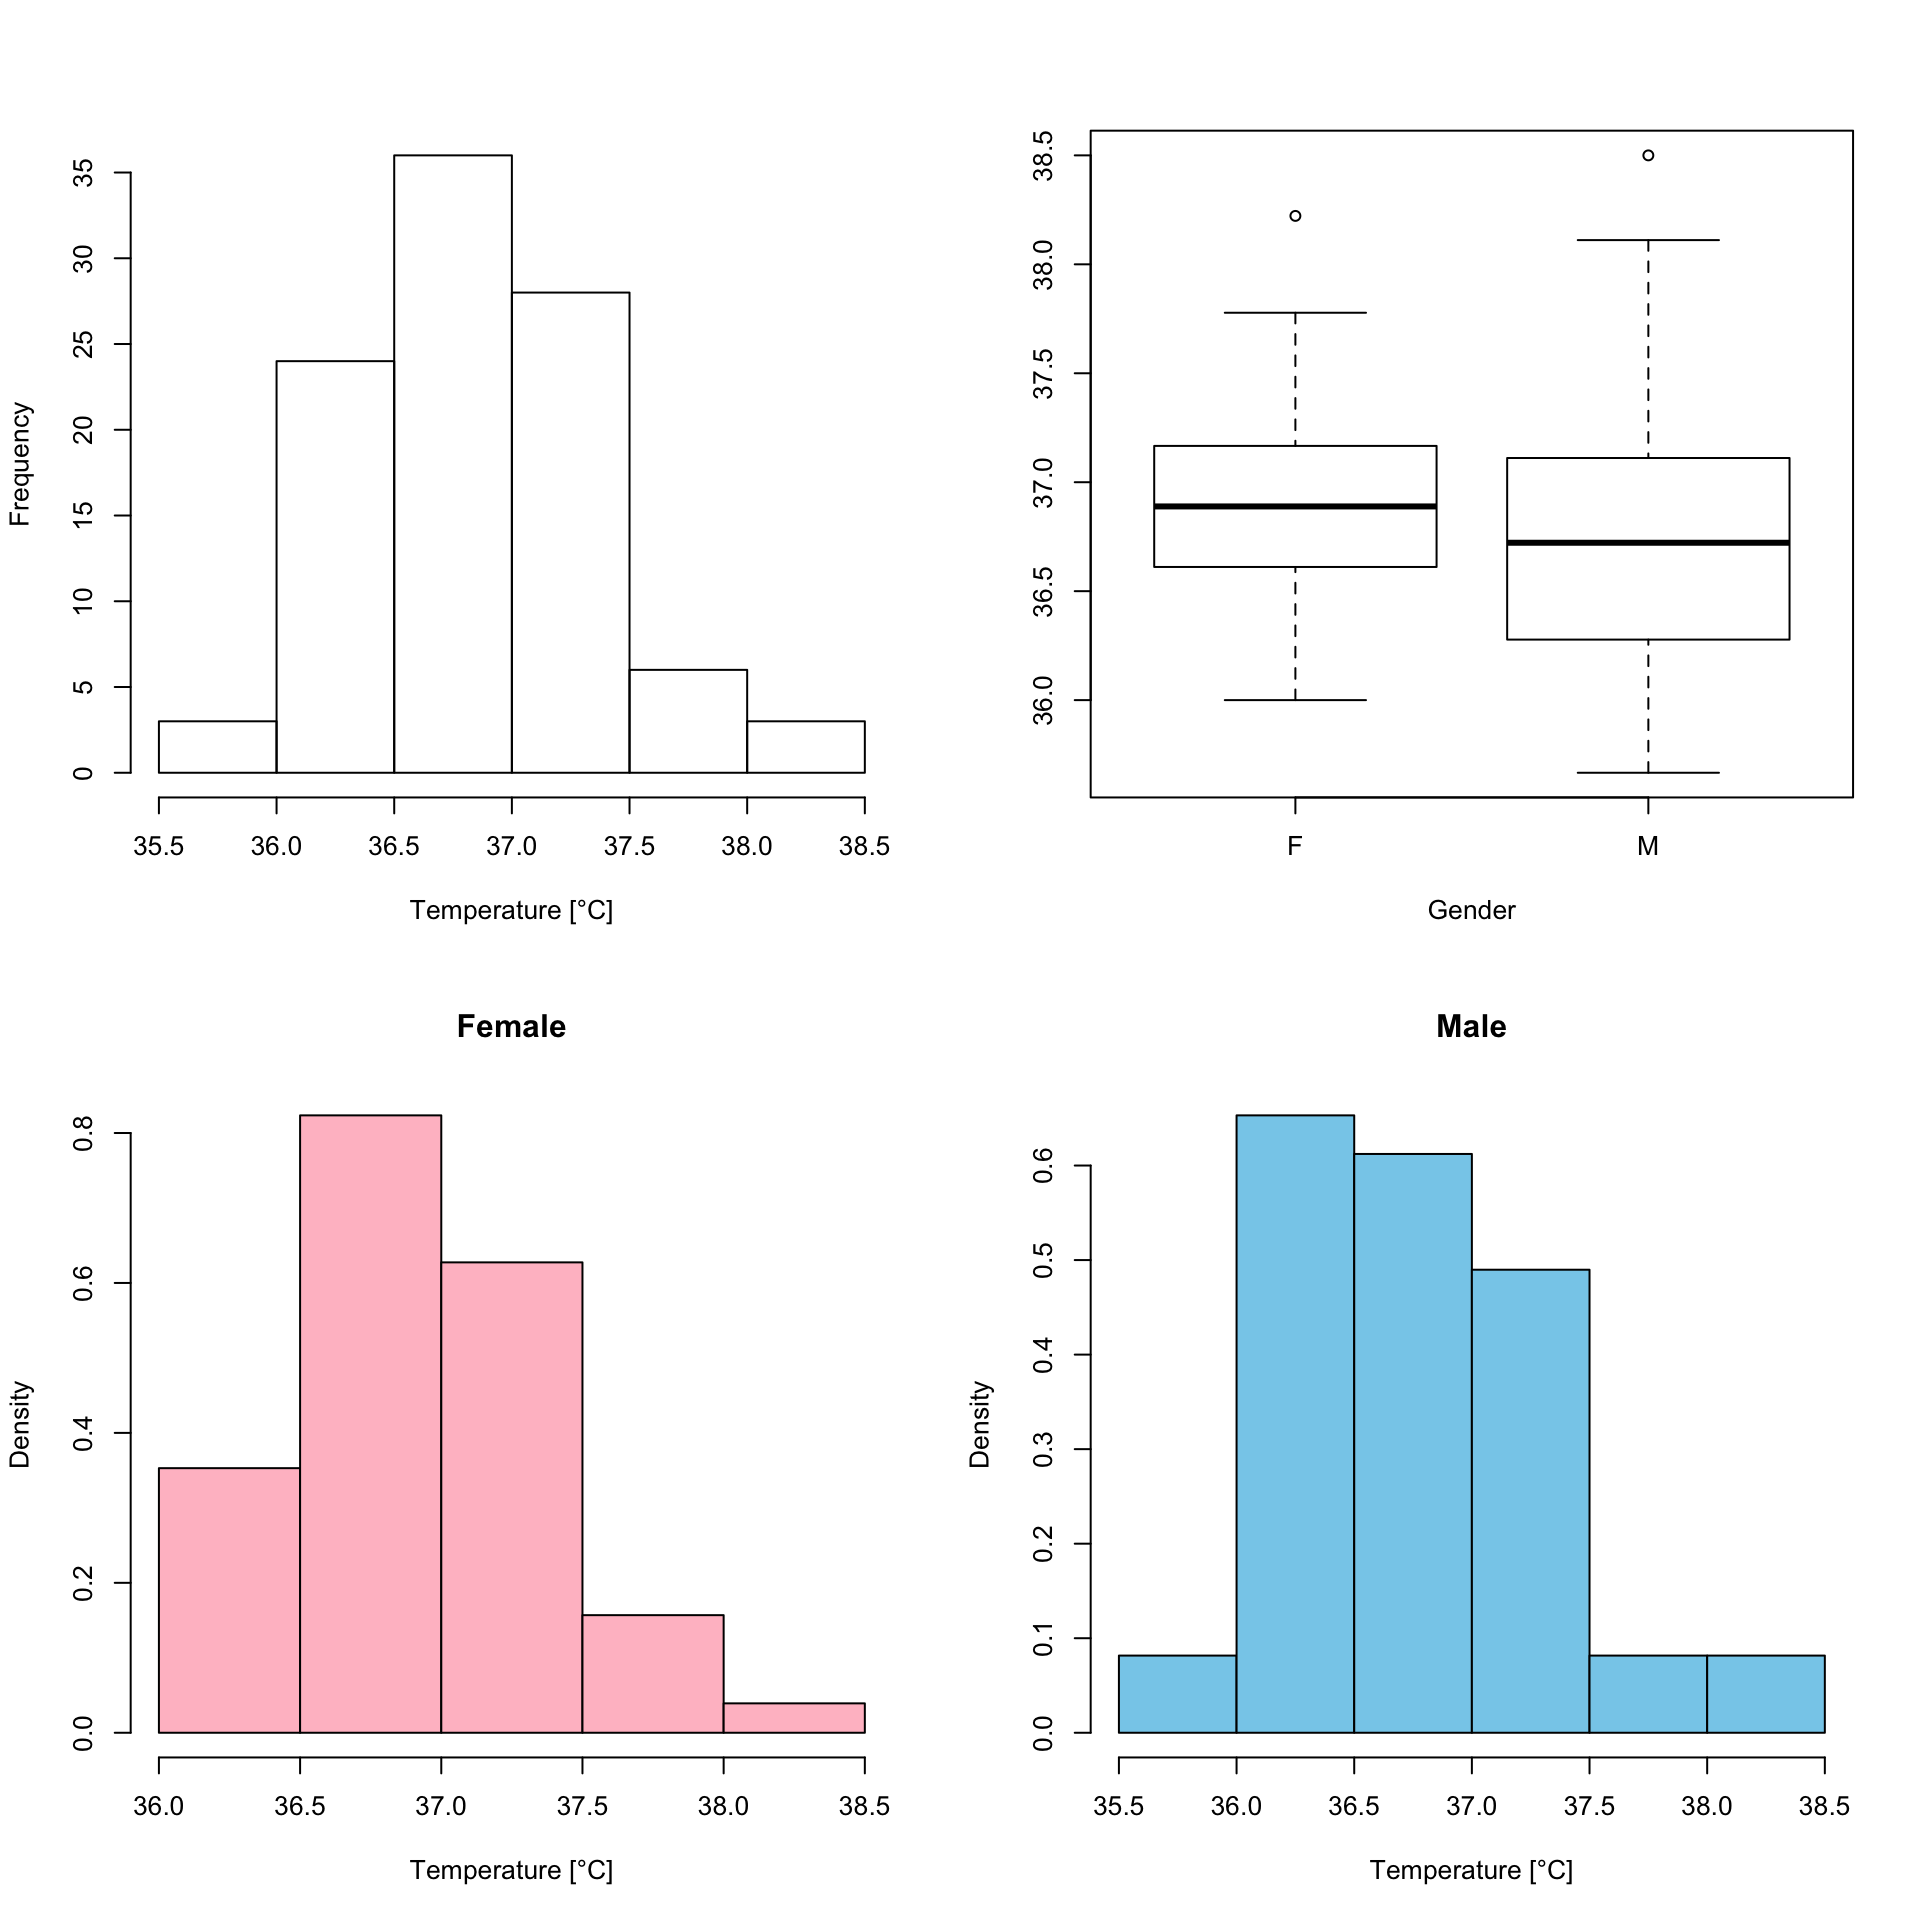
\includegraphics{bookdown_files/figure-latex/unnamed-chunk-53-1.pdf}

Esistono altri comandi che si possono abbinare a quelli di visualizzazione visti fin qui, ad esempio \texttt{abline()}, \texttt{text()} e \texttt{lines()}.

\emph{Esercizio} Usare l'help per capire le funzionalità dei comandi precedenti e si usino per aggiungere informazioni ai grafici precedenti.

\hypertarget{analizzare-il-dataset-pima.tr2}{%
\section{Analizzare il dataset Pima.tr2}\label{analizzare-il-dataset-pima.tr2}}

\begin{Shaded}
\begin{Highlighting}[]
\KeywordTok{library}\NormalTok{(MASS) }\CommentTok{# necessario per accedere al dataset}
\KeywordTok{str}\NormalTok{(Pima.tr2)}
\end{Highlighting}
\end{Shaded}

\begin{verbatim}
## 'data.frame':    300 obs. of  8 variables:
##  $ npreg: int  5 7 5 0 0 5 3 1 3 2 ...
##  $ glu  : int  86 195 77 165 107 97 83 193 142 128 ...
##  $ bp   : int  68 70 82 76 60 76 58 50 80 78 ...
##  $ skin : int  28 33 41 43 25 27 31 16 15 37 ...
##  $ bmi  : num  30.2 25.1 35.8 47.9 26.4 35.6 34.3 25.9 32.4 43.3 ...
##  $ ped  : num  0.364 0.163 0.156 0.259 0.133 ...
##  $ age  : int  24 55 35 26 23 52 25 24 63 31 ...
##  $ type : Factor w/ 2 levels "No","Yes": 1 2 1 1 1 2 1 1 1 2 ...
\end{verbatim}

\begin{Shaded}
\begin{Highlighting}[]
\KeywordTok{dim}\NormalTok{(Pima.tr2)}
\end{Highlighting}
\end{Shaded}

\begin{verbatim}
## [1] 300   8
\end{verbatim}

\begin{Shaded}
\begin{Highlighting}[]
\KeywordTok{names}\NormalTok{(Pima.tr2)}
\end{Highlighting}
\end{Shaded}

\begin{verbatim}
## [1] "npreg" "glu"   "bp"    "skin"  "bmi"   "ped"   "age"   "type"
\end{verbatim}

\begin{Shaded}
\begin{Highlighting}[]
\NormalTok{?Pima.tr2}
\KeywordTok{head}\NormalTok{(Pima.tr2)}
\end{Highlighting}
\end{Shaded}

\begin{verbatim}
##   npreg glu bp skin  bmi   ped age type
## 1     5  86 68   28 30.2 0.364  24   No
## 2     7 195 70   33 25.1 0.163  55  Yes
## 3     5  77 82   41 35.8 0.156  35   No
## 4     0 165 76   43 47.9 0.259  26   No
## 5     0 107 60   25 26.4 0.133  23   No
## 6     5  97 76   27 35.6 0.378  52  Yes
\end{verbatim}

\begin{Shaded}
\begin{Highlighting}[]
\KeywordTok{summary}\NormalTok{(Pima.tr2)}
\end{Highlighting}
\end{Shaded}

\begin{verbatim}
##      npreg             glu              bp              skin      
##  Min.   : 0.000   Min.   : 56.0   Min.   : 38.00   Min.   : 7.00  
##  1st Qu.: 1.000   1st Qu.:101.0   1st Qu.: 64.00   1st Qu.:21.00  
##  Median : 3.000   Median :121.0   Median : 72.00   Median :29.00  
##  Mean   : 3.787   Mean   :123.7   Mean   : 72.32   Mean   :29.15  
##  3rd Qu.: 6.000   3rd Qu.:142.0   3rd Qu.: 80.00   3rd Qu.:36.00  
##  Max.   :14.000   Max.   :199.0   Max.   :114.00   Max.   :99.00  
##                                   NA's   :13       NA's   :98     
##       bmi             ped              age        type    
##  Min.   :18.20   Min.   :0.0780   Min.   :21.0   No :194  
##  1st Qu.:27.10   1st Qu.:0.2367   1st Qu.:24.0   Yes:106  
##  Median :32.00   Median :0.3360   Median :29.0            
##  Mean   :32.05   Mean   :0.4357   Mean   :33.1            
##  3rd Qu.:36.50   3rd Qu.:0.5867   3rd Qu.:40.0            
##  Max.   :52.90   Max.   :2.2880   Max.   :72.0            
##  NA's   :3
\end{verbatim}

\begin{Shaded}
\begin{Highlighting}[]
\KeywordTok{which}\NormalTok{(}\KeywordTok{is.na}\NormalTok{(Pima.tr2))}
\end{Highlighting}
\end{Shaded}

\begin{verbatim}
##   [1]  804  834  836  853  854  863  871  885  887  888  889  898  899 1101
##  [15] 1102 1103 1104 1105 1106 1107 1108 1109 1110 1111 1112 1113 1114 1115
##  [29] 1116 1117 1118 1119 1120 1121 1122 1123 1124 1125 1126 1127 1128 1129
##  [43] 1131 1132 1133 1134 1135 1136 1137 1138 1139 1140 1141 1142 1143 1144
##  [57] 1145 1146 1147 1148 1149 1150 1151 1152 1153 1154 1155 1156 1157 1158
##  [71] 1159 1160 1161 1162 1163 1164 1165 1166 1167 1168 1169 1170 1172 1173
##  [85] 1174 1175 1176 1177 1178 1179 1180 1181 1182 1183 1184 1185 1186 1187
##  [99] 1188 1189 1190 1191 1192 1193 1194 1195 1196 1197 1198 1199 1200 1413
## [113] 1430 1468
\end{verbatim}

\begin{Shaded}
\begin{Highlighting}[]
\CommentTok{# amico di apply}
\KeywordTok{lapply}\NormalTok{(}\KeywordTok{lapply}\NormalTok{(Pima.tr2 , is.na),which)}
\end{Highlighting}
\end{Shaded}

\begin{verbatim}
## $npreg
## integer(0)
## 
## $glu
## integer(0)
## 
## $bp
##  [1] 204 234 236 253 254 263 271 285 287 288 289 298 299
## 
## $skin
##  [1] 201 202 203 204 205 206 207 208 209 210 211 212 213 214 215 216 217
## [18] 218 219 220 221 222 223 224 225 226 227 228 229 231 232 233 234 235
## [35] 236 237 238 239 240 241 242 243 244 245 246 247 248 249 250 251 252
## [52] 253 254 255 256 257 258 259 260 261 262 263 264 265 266 267 268 269
## [69] 270 272 273 274 275 276 277 278 279 280 281 282 283 284 285 286 287
## [86] 288 289 290 291 292 293 294 295 296 297 298 299 300
## 
## $bmi
## [1] 213 230 268
## 
## $ped
## integer(0)
## 
## $age
## integer(0)
## 
## $type
## integer(0)
\end{verbatim}

Cosa possiamo fare con i diversi NA?

Un'idea ovviamente è quella di rimuovere le righe dove compare un NA

\begin{Shaded}
\begin{Highlighting}[]
\NormalTok{data_no_Na <-}\StringTok{ }\KeywordTok{na.omit}\NormalTok{(Pima.tr2)}

\KeywordTok{dim}\NormalTok{(data_no_Na)}
\end{Highlighting}
\end{Shaded}

\begin{verbatim}
## [1] 200   8
\end{verbatim}

Abbiamo rimosso un terzo del dataset\ldots{}..

Rimuovere così tanti dati impoverisce significativamente il dataset, quindi magari si possono trovare soluzioni meno radicali.

Ad esempio, possiamo notare come gran parte dei NA siano nella variabile \emph{skin}\ldots{} se questa non ci interessa, possiamo evitare di rimuovere quelle righe!

\begin{Shaded}
\begin{Highlighting}[]
\NormalTok{data_no_Na <-}\StringTok{ }\KeywordTok{na.omit}\NormalTok{(Pima.tr2[,}\OperatorTok{-}\DecValTok{4}\NormalTok{])}

\KeywordTok{dim}\NormalTok{(data_no_Na)}
\end{Highlighting}
\end{Shaded}

\begin{verbatim}
## [1] 284   7
\end{verbatim}

In questo modo abbiamo rimosso molte meno righe.
Si noti che alcune funzioni (vedi mean) hanno specifici argomenti per gestire i NA e si può quindi evitare di rimuoverli dal dataset ma gestirli i vari casi dalle funzioni

In alcuni casi, si preferisce non rimuovere alcun dato, ma piuttosto si sostituiscono i valori mancanti con informazioni prese dai dati correnti.

Ad esempio, si possono sostituire con la media, la mediana o si possono anche definire modelli più complessi per definire i sostituti.

\hypertarget{visualizzare-il-dataset-pima.tr2}{%
\section{Visualizzare il dataset Pima.tr2}\label{visualizzare-il-dataset-pima.tr2}}

Usando gli strumenti di visualizzazione visti, si esplorino le relazioni tra le variabili del dataset.

Si faccia attenzione agli NA e si confrontino i risultati nei casi in cui:

\begin{itemize}
\tightlist
\item
  vengono rimosse tutte le righe contenenti NA;
\item
  vengono solo le righe contenenti NA nelle variabili di interesse;
\item
  vengono sostituiti gli NA con la media o la mediana della variabile;
\end{itemize}

\hypertarget{esercizi-1}{%
\section{Esercizi}\label{esercizi-1}}

\hypertarget{esercizio-1-1}{%
\subsection{Esercizio 1}\label{esercizio-1-1}}

Si scarichi il dataset \href{http://extras.springer.com/2012/978-1-4614-1301-1}{AstmaLOS.txt} (\href{https://www.dropbox.com/s/kjhafwojufpwaga/AsthmaLOS_description.txt?dl=0}{descrizione}). Dopo averlo analizzato ed aver individuato eventuali errori nei dati relativi ad age e owner.type, si analizzi e visualizzi la variabile age. Si provino almeno due tecniche di rimozione degli errori dai dati e si confrontino i risultati.

\hypertarget{esercizio-2-1}{%
\subsection{Esercizio 2}\label{esercizio-2-1}}

Si analizzi il dataset \emph{hflights} e si scelga una destinazione. Si analizzino e visualizzino i dati relativi a lunghezza del volo e ritardi per tale destinazione. Inoltre si determini:

\begin{itemize}
\tightlist
\item
  il giorno in cui è possibile volare con minore probabilità di subire ritardo.
\item
  il giorno in cui è possibile volare con maggiore probabilità di subire la cancellazione del volo.
\end{itemize}

\hypertarget{link-utili-2}{%
\section{Link utili}\label{link-utili-2}}

\begin{itemize}
\item
  Questo sito presenta diversi \href{http://college.cengage.com/mathematics/brase/understandable_statistics/7e/students/datasets/slr/frames/frame.html}{datasets} che possono essere interessanti da esaminare.
\item
  A questo link è possibile trovare gli appunti di un ottimo corso di \href{http://vissoc.co}{data visualization} (in inglese).
\end{itemize}

\hypertarget{fare-pratica-con-i-dati}{%
\chapter{Fare pratica con i dati}\label{fare-pratica-con-i-dati}}

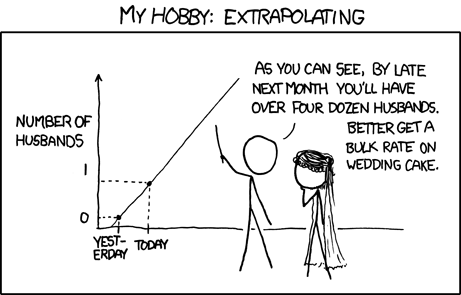
\includegraphics{media/extrapolating.png}
Originally posted \href{https://xkcd.com/605/}{here}.

\hypertarget{inquinamento-a-san-andreas}{%
\section{Inquinamento a San Andreas}\label{inquinamento-a-san-andreas}}

Iniziamo scaricando il dataset dal \href{https://www.dropbox.com/s/9zx2dtne9gnafcm/PM10dataSanAndreas.csv?dl=1}{link} dove ho isolato (e pulito) i dati raccolti dall'agenzia americana per la tutela dell'ambiente, relativi alle rilevazioni orarie della concentrazione delle PM10 nell'aria nella città di San Andreas, CA.

Questo dataset è una parte di un dataset molto più grande che si può trovare al \href{http://aqsdr1.epa.gov/aqsweb/aqstmp/airdata/download_files.html\#Raw}{link}. Queste analisi sono ispirate a \citep{Peng2015}.

Una volta salvato il file nella nostra cartella \emph{data} passiamo a leggere il suo contenuto.

\begin{Shaded}
\begin{Highlighting}[]
\NormalTok{PM10dataSA <-}\StringTok{ }\KeywordTok{read.csv}\NormalTok{(}\StringTok{"./data/PM10dataSanAndreas.csv"}\NormalTok{)}
\NormalTok{knitr}\OperatorTok{::}\KeywordTok{kable}\NormalTok{(}
\KeywordTok{head}\NormalTok{(PM10dataSA),}
\DataTypeTok{booktabs =} \OtherTok{TRUE}
\NormalTok{)}
\end{Highlighting}
\end{Shaded}

\begin{tabular}{rrrrrrrrrrllllllrlrlllrlllll}
\toprule
X.2 & X.1 & X & State.Code & County.Code & Site.Num & Parameter.Code & POC & Latitude & Longitude & Datum & Parameter.Name & Date.Local & Time.Local & Date.GMT & Time.GMT & Sample.Measurement & Units.of.Measure & MDL & Uncertainty & Qualifier & Method.Type & Method.Code & Method.Name & State.Name & County.Name & Date.of.Last.Change & DateTime.Local\\
\midrule
1 & 1 & 308088 & 6 & 9 & 1 & 81102 & 3 & 38.20185 & -120.6816 & WGS84 & PM10 Total 0-10um STP & 2016-01-01 & 00:00 & 2016-01-01 & 08:00 & 25 & Micrograms/cubic meter (25 C) & 4 & NA & NA & FEM & 122 & INSTRUMENT MET ONE 4 MODELS - BETA ATTENUATION & California & Calaveras & 2016-05-06 & 2016-01-01 00:00:00\\
2 & 2 & 308089 & 6 & 9 & 1 & 81102 & 3 & 38.20185 & -120.6816 & WGS84 & PM10 Total 0-10um STP & 2016-01-01 & 01:00 & 2016-01-01 & 09:00 & 48 & Micrograms/cubic meter (25 C) & 4 & NA & NA & FEM & 122 & INSTRUMENT MET ONE 4 MODELS - BETA ATTENUATION & California & Calaveras & 2016-05-06 & 2016-01-01 01:00:00\\
3 & 3 & 308090 & 6 & 9 & 1 & 81102 & 3 & 38.20185 & -120.6816 & WGS84 & PM10 Total 0-10um STP & 2016-01-01 & 02:00 & 2016-01-01 & 10:00 & 26 & Micrograms/cubic meter (25 C) & 4 & NA & NA & FEM & 122 & INSTRUMENT MET ONE 4 MODELS - BETA ATTENUATION & California & Calaveras & 2016-05-06 & 2016-01-01 02:00:00\\
4 & 4 & 308091 & 6 & 9 & 1 & 81102 & 3 & 38.20185 & -120.6816 & WGS84 & PM10 Total 0-10um STP & 2016-01-01 & 03:00 & 2016-01-01 & 11:00 & 14 & Micrograms/cubic meter (25 C) & 4 & NA & NA & FEM & 122 & INSTRUMENT MET ONE 4 MODELS - BETA ATTENUATION & California & Calaveras & 2016-05-06 & 2016-01-01 03:00:00\\
5 & 5 & 308092 & 6 & 9 & 1 & 81102 & 3 & 38.20185 & -120.6816 & WGS84 & PM10 Total 0-10um STP & 2016-01-01 & 04:00 & 2016-01-01 & 12:00 & 7 & Micrograms/cubic meter (25 C) & 4 & NA & NA & FEM & 122 & INSTRUMENT MET ONE 4 MODELS - BETA ATTENUATION & California & Calaveras & 2016-05-06 & 2016-01-01 04:00:00\\
\addlinespace
6 & 6 & 308093 & 6 & 9 & 1 & 81102 & 3 & 38.20185 & -120.6816 & WGS84 & PM10 Total 0-10um STP & 2016-01-01 & 05:00 & 2016-01-01 & 13:00 & 14 & Micrograms/cubic meter (25 C) & 4 & NA & NA & FEM & 122 & INSTRUMENT MET ONE 4 MODELS - BETA ATTENUATION & California & Calaveras & 2016-05-06 & 2016-01-01 05:00:00\\
\bottomrule
\end{tabular}

Possiamo iniziare a prendere confidenza con il dataset leggendo alcune informazioni essenziali, come la dimensione, il nome delle variabili, oppure ne possiamo esplorare la struttura, visualizzare le prime o le ultime righe.

\begin{Shaded}
\begin{Highlighting}[]
\KeywordTok{dim}\NormalTok{(PM10dataSA)}
\end{Highlighting}
\end{Shaded}

\begin{verbatim}
## [1] 2581   28
\end{verbatim}

Vediamo subito che il dataset contiene più di 2mila osservazioni per 26 variabili. Accediamo i nomi delle variabili per vedere se riusciamo a capirne il significato.

\begin{Shaded}
\begin{Highlighting}[]
\KeywordTok{names}\NormalTok{(PM10dataSA)}
\end{Highlighting}
\end{Shaded}

\begin{verbatim}
##  [1] "X.2"                 "X.1"                 "X"                  
##  [4] "State.Code"          "County.Code"         "Site.Num"           
##  [7] "Parameter.Code"      "POC"                 "Latitude"           
## [10] "Longitude"           "Datum"               "Parameter.Name"     
## [13] "Date.Local"          "Time.Local"          "Date.GMT"           
## [16] "Time.GMT"            "Sample.Measurement"  "Units.of.Measure"   
## [19] "MDL"                 "Uncertainty"         "Qualifier"          
## [22] "Method.Type"         "Method.Code"         "Method.Name"        
## [25] "State.Name"          "County.Name"         "Date.of.Last.Change"
## [28] "DateTime.Local"
\end{verbatim}

Proseguiamo visualizzando la struttura ed alcune righe dei dati.

\begin{Shaded}
\begin{Highlighting}[]
\KeywordTok{str}\NormalTok{(PM10dataSA)}
\end{Highlighting}
\end{Shaded}

\begin{verbatim}
## 'data.frame':    2581 obs. of  28 variables:
##  $ X.2                : int  1 2 3 4 5 6 7 8 9 10 ...
##  $ X.1                : int  1 2 3 4 5 6 7 8 9 10 ...
##  $ X                  : int  308088 308089 308090 308091 308092 308093 308094 308095 308096 308097 ...
##  $ State.Code         : int  6 6 6 6 6 6 6 6 6 6 ...
##  $ County.Code        : int  9 9 9 9 9 9 9 9 9 9 ...
##  $ Site.Num           : int  1 1 1 1 1 1 1 1 1 1 ...
##  $ Parameter.Code     : int  81102 81102 81102 81102 81102 81102 81102 81102 81102 81102 ...
##  $ POC                : int  3 3 3 3 3 3 3 3 3 3 ...
##  $ Latitude           : num  38.2 38.2 38.2 38.2 38.2 ...
##  $ Longitude          : num  -121 -121 -121 -121 -121 ...
##  $ Datum              : Factor w/ 1 level "WGS84": 1 1 1 1 1 1 1 1 1 1 ...
##  $ Parameter.Name     : Factor w/ 1 level "PM10 Total 0-10um STP": 1 1 1 1 1 1 1 1 1 1 ...
##  $ Date.Local         : Factor w/ 120 levels "2016-01-01","2016-01-02",..: 1 1 1 1 1 1 1 1 1 1 ...
##  $ Time.Local         : Factor w/ 24 levels "00:00","01:00",..: 1 2 3 4 5 6 7 8 9 10 ...
##  $ Date.GMT           : Factor w/ 122 levels "2016-01-01","2016-01-02",..: 1 1 1 1 1 1 1 1 1 1 ...
##  $ Time.GMT           : Factor w/ 24 levels "00:00","01:00",..: 9 10 11 12 13 14 15 16 17 18 ...
##  $ Sample.Measurement : int  25 48 26 14 7 14 11 16 17 11 ...
##  $ Units.of.Measure   : Factor w/ 1 level "Micrograms/cubic meter (25 C)": 1 1 1 1 1 1 1 1 1 1 ...
##  $ MDL                : int  4 4 4 4 4 4 4 4 4 4 ...
##  $ Uncertainty        : logi  NA NA NA NA NA NA ...
##  $ Qualifier          : logi  NA NA NA NA NA NA ...
##  $ Method.Type        : Factor w/ 1 level "FEM": 1 1 1 1 1 1 1 1 1 1 ...
##  $ Method.Code        : int  122 122 122 122 122 122 122 122 122 122 ...
##  $ Method.Name        : Factor w/ 1 level "INSTRUMENT MET ONE 4 MODELS - BETA ATTENUATION": 1 1 1 1 1 1 1 1 1 1 ...
##  $ State.Name         : Factor w/ 1 level "California": 1 1 1 1 1 1 1 1 1 1 ...
##  $ County.Name        : Factor w/ 1 level "Calaveras": 1 1 1 1 1 1 1 1 1 1 ...
##  $ Date.of.Last.Change: Factor w/ 4 levels "2016-05-06","2016-05-12",..: 1 1 1 1 1 1 1 1 1 1 ...
##  $ DateTime.Local     : Factor w/ 2580 levels "2016-01-01 00:00:00",..: 1 2 3 4 5 6 7 8 9 10 ...
\end{verbatim}

\begin{Shaded}
\begin{Highlighting}[]
\NormalTok{knitr}\OperatorTok{::}\KeywordTok{kable}\NormalTok{(}
\KeywordTok{head}\NormalTok{(PM10dataSA),}
\DataTypeTok{booktabs =} \OtherTok{TRUE}
\NormalTok{)}
\end{Highlighting}
\end{Shaded}

\begin{tabular}{rrrrrrrrrrllllllrlrlllrlllll}
\toprule
X.2 & X.1 & X & State.Code & County.Code & Site.Num & Parameter.Code & POC & Latitude & Longitude & Datum & Parameter.Name & Date.Local & Time.Local & Date.GMT & Time.GMT & Sample.Measurement & Units.of.Measure & MDL & Uncertainty & Qualifier & Method.Type & Method.Code & Method.Name & State.Name & County.Name & Date.of.Last.Change & DateTime.Local\\
\midrule
1 & 1 & 308088 & 6 & 9 & 1 & 81102 & 3 & 38.20185 & -120.6816 & WGS84 & PM10 Total 0-10um STP & 2016-01-01 & 00:00 & 2016-01-01 & 08:00 & 25 & Micrograms/cubic meter (25 C) & 4 & NA & NA & FEM & 122 & INSTRUMENT MET ONE 4 MODELS - BETA ATTENUATION & California & Calaveras & 2016-05-06 & 2016-01-01 00:00:00\\
2 & 2 & 308089 & 6 & 9 & 1 & 81102 & 3 & 38.20185 & -120.6816 & WGS84 & PM10 Total 0-10um STP & 2016-01-01 & 01:00 & 2016-01-01 & 09:00 & 48 & Micrograms/cubic meter (25 C) & 4 & NA & NA & FEM & 122 & INSTRUMENT MET ONE 4 MODELS - BETA ATTENUATION & California & Calaveras & 2016-05-06 & 2016-01-01 01:00:00\\
3 & 3 & 308090 & 6 & 9 & 1 & 81102 & 3 & 38.20185 & -120.6816 & WGS84 & PM10 Total 0-10um STP & 2016-01-01 & 02:00 & 2016-01-01 & 10:00 & 26 & Micrograms/cubic meter (25 C) & 4 & NA & NA & FEM & 122 & INSTRUMENT MET ONE 4 MODELS - BETA ATTENUATION & California & Calaveras & 2016-05-06 & 2016-01-01 02:00:00\\
4 & 4 & 308091 & 6 & 9 & 1 & 81102 & 3 & 38.20185 & -120.6816 & WGS84 & PM10 Total 0-10um STP & 2016-01-01 & 03:00 & 2016-01-01 & 11:00 & 14 & Micrograms/cubic meter (25 C) & 4 & NA & NA & FEM & 122 & INSTRUMENT MET ONE 4 MODELS - BETA ATTENUATION & California & Calaveras & 2016-05-06 & 2016-01-01 03:00:00\\
5 & 5 & 308092 & 6 & 9 & 1 & 81102 & 3 & 38.20185 & -120.6816 & WGS84 & PM10 Total 0-10um STP & 2016-01-01 & 04:00 & 2016-01-01 & 12:00 & 7 & Micrograms/cubic meter (25 C) & 4 & NA & NA & FEM & 122 & INSTRUMENT MET ONE 4 MODELS - BETA ATTENUATION & California & Calaveras & 2016-05-06 & 2016-01-01 04:00:00\\
\addlinespace
6 & 6 & 308093 & 6 & 9 & 1 & 81102 & 3 & 38.20185 & -120.6816 & WGS84 & PM10 Total 0-10um STP & 2016-01-01 & 05:00 & 2016-01-01 & 13:00 & 14 & Micrograms/cubic meter (25 C) & 4 & NA & NA & FEM & 122 & INSTRUMENT MET ONE 4 MODELS - BETA ATTENUATION & California & Calaveras & 2016-05-06 & 2016-01-01 05:00:00\\
\bottomrule
\end{tabular}

\begin{Shaded}
\begin{Highlighting}[]
\NormalTok{knitr}\OperatorTok{::}\KeywordTok{kable}\NormalTok{(}
\KeywordTok{tail}\NormalTok{(PM10dataSA),}
\DataTypeTok{booktabs =} \OtherTok{TRUE}
\NormalTok{)}
\end{Highlighting}
\end{Shaded}

\begin{tabular}{lrrrrrrrrrrllllllrlrlllrlllll}
\toprule
  & X.2 & X.1 & X & State.Code & County.Code & Site.Num & Parameter.Code & POC & Latitude & Longitude & Datum & Parameter.Name & Date.Local & Time.Local & Date.GMT & Time.GMT & Sample.Measurement & Units.of.Measure & MDL & Uncertainty & Qualifier & Method.Type & Method.Code & Method.Name & State.Name & County.Name & Date.of.Last.Change & DateTime.Local\\
\midrule
2576 & 2576 & 2862 & 310949 & 6 & 9 & 1 & 81102 & 3 & 38.20185 & -120.6816 & WGS84 & PM10 Total 0-10um STP & 2016-04-30 & 18:00 & 2016-05-01 & 02:00 & 15 & Micrograms/cubic meter (25 C) & 4 & NA & NA & FEM & 122 & INSTRUMENT MET ONE 4 MODELS - BETA ATTENUATION & California & Calaveras & 2016-11-08 & 2016-04-30 18:00:00\\
2577 & 2577 & 2863 & 310950 & 6 & 9 & 1 & 81102 & 3 & 38.20185 & -120.6816 & WGS84 & PM10 Total 0-10um STP & 2016-04-30 & 19:00 & 2016-05-01 & 03:00 & 13 & Micrograms/cubic meter (25 C) & 4 & NA & NA & FEM & 122 & INSTRUMENT MET ONE 4 MODELS - BETA ATTENUATION & California & Calaveras & 2016-11-08 & 2016-04-30 19:00:00\\
2578 & 2578 & 2864 & 310951 & 6 & 9 & 1 & 81102 & 3 & 38.20185 & -120.6816 & WGS84 & PM10 Total 0-10um STP & 2016-04-30 & 20:00 & 2016-05-01 & 04:00 & 9 & Micrograms/cubic meter (25 C) & 4 & NA & NA & FEM & 122 & INSTRUMENT MET ONE 4 MODELS - BETA ATTENUATION & California & Calaveras & 2016-11-08 & 2016-04-30 20:00:00\\
2579 & 2579 & 2865 & 310952 & 6 & 9 & 1 & 81102 & 3 & 38.20185 & -120.6816 & WGS84 & PM10 Total 0-10um STP & 2016-04-30 & 21:00 & 2016-05-01 & 05:00 & 4 & Micrograms/cubic meter (25 C) & 4 & NA & NA & FEM & 122 & INSTRUMENT MET ONE 4 MODELS - BETA ATTENUATION & California & Calaveras & 2016-11-08 & 2016-04-30 21:00:00\\
2580 & 2580 & 2866 & 310953 & 6 & 9 & 1 & 81102 & 3 & 38.20185 & -120.6816 & WGS84 & PM10 Total 0-10um STP & 2016-04-30 & 22:00 & 2016-05-01 & 06:00 & 6 & Micrograms/cubic meter (25 C) & 4 & NA & NA & FEM & 122 & INSTRUMENT MET ONE 4 MODELS - BETA ATTENUATION & California & Calaveras & 2016-11-08 & 2016-04-30 22:00:00\\
\addlinespace
2581 & 2581 & 2867 & 310954 & 6 & 9 & 1 & 81102 & 3 & 38.20185 & -120.6816 & WGS84 & PM10 Total 0-10um STP & 2016-04-30 & 23:00 & 2016-05-01 & 07:00 & 4 & Micrograms/cubic meter (25 C) & 4 & NA & NA & FEM & 122 & INSTRUMENT MET ONE 4 MODELS - BETA ATTENUATION & California & Calaveras & 2016-11-08 & 2016-04-30 23:00:00\\
\bottomrule
\end{tabular}

Vediamo che i dati contengono indicazioni come coordinate geografiche e lo stato dove sono stati raccolti i dati. Nel caso del dataset originale, queste informazioni sono essenziali per individuare il luogo di raccolta dati, mentre nel nostro caso potrebbero essere omesse, \textbf{dopo} aver verificato che siano consistenti in tutto il dataset.

Siamo interessati a capire l'andamento delle PM10 nel nostro dataset durante il tempo in cui sono stati raccolti i dati. Per prima cosa convertiamo i dati riguardanti le date nel giusto formato, cioè in \emph{Date}. Usiamo per ora solo le informazioni relative al fuso orario locale.

\begin{Shaded}
\begin{Highlighting}[]
\NormalTok{PM10dataSA}\OperatorTok{$}\NormalTok{Date.Local <-}\StringTok{ }\KeywordTok{as.Date}\NormalTok{(PM10dataSA}\OperatorTok{$}\NormalTok{Date.Local)}
\end{Highlighting}
\end{Shaded}

Ora che i dati sono in formato \emph{Date}, R capisce che sono numeri salvati con un particolare formato e non stringhe.

In questo modo possiamo, ad esempio, vedere il periodo temporale che coprono usano i comandi min e max.

\begin{Shaded}
\begin{Highlighting}[]
\KeywordTok{paste}\NormalTok{(}\KeywordTok{min}\NormalTok{(PM10dataSA}\OperatorTok{$}\NormalTok{Date.Local), }\KeywordTok{which.min}\NormalTok{(PM10dataSA}\OperatorTok{$}\NormalTok{Date.Local))}
\end{Highlighting}
\end{Shaded}

\begin{verbatim}
## [1] "2016-01-01 1"
\end{verbatim}

\begin{Shaded}
\begin{Highlighting}[]
\KeywordTok{paste}\NormalTok{(}\KeywordTok{max}\NormalTok{(PM10dataSA}\OperatorTok{$}\NormalTok{Date.Local), }\KeywordTok{which.max}\NormalTok{(PM10dataSA}\OperatorTok{$}\NormalTok{Date.Local))}
\end{Highlighting}
\end{Shaded}

\begin{verbatim}
## [1] "2016-04-30 2559"
\end{verbatim}

Possiamo notare che il dataset non supera Aprile e che il max non è assunto nell'ultima osservazione, che sarebbe la 2867. Usando il comando \texttt{tail()} vediamo di capire perché.

\begin{Shaded}
\begin{Highlighting}[]
\NormalTok{knitr}\OperatorTok{::}\KeywordTok{kable}\NormalTok{(}
\KeywordTok{tail}\NormalTok{(PM10dataSA),}
\DataTypeTok{booktabs =} \OtherTok{TRUE}
\NormalTok{)}
\end{Highlighting}
\end{Shaded}

\begin{tabular}{lrrrrrrrrrrllllllrlrlllrlllll}
\toprule
  & X.2 & X.1 & X & State.Code & County.Code & Site.Num & Parameter.Code & POC & Latitude & Longitude & Datum & Parameter.Name & Date.Local & Time.Local & Date.GMT & Time.GMT & Sample.Measurement & Units.of.Measure & MDL & Uncertainty & Qualifier & Method.Type & Method.Code & Method.Name & State.Name & County.Name & Date.of.Last.Change & DateTime.Local\\
\midrule
2576 & 2576 & 2862 & 310949 & 6 & 9 & 1 & 81102 & 3 & 38.20185 & -120.6816 & WGS84 & PM10 Total 0-10um STP & 2016-04-30 & 18:00 & 2016-05-01 & 02:00 & 15 & Micrograms/cubic meter (25 C) & 4 & NA & NA & FEM & 122 & INSTRUMENT MET ONE 4 MODELS - BETA ATTENUATION & California & Calaveras & 2016-11-08 & 2016-04-30 18:00:00\\
2577 & 2577 & 2863 & 310950 & 6 & 9 & 1 & 81102 & 3 & 38.20185 & -120.6816 & WGS84 & PM10 Total 0-10um STP & 2016-04-30 & 19:00 & 2016-05-01 & 03:00 & 13 & Micrograms/cubic meter (25 C) & 4 & NA & NA & FEM & 122 & INSTRUMENT MET ONE 4 MODELS - BETA ATTENUATION & California & Calaveras & 2016-11-08 & 2016-04-30 19:00:00\\
2578 & 2578 & 2864 & 310951 & 6 & 9 & 1 & 81102 & 3 & 38.20185 & -120.6816 & WGS84 & PM10 Total 0-10um STP & 2016-04-30 & 20:00 & 2016-05-01 & 04:00 & 9 & Micrograms/cubic meter (25 C) & 4 & NA & NA & FEM & 122 & INSTRUMENT MET ONE 4 MODELS - BETA ATTENUATION & California & Calaveras & 2016-11-08 & 2016-04-30 20:00:00\\
2579 & 2579 & 2865 & 310952 & 6 & 9 & 1 & 81102 & 3 & 38.20185 & -120.6816 & WGS84 & PM10 Total 0-10um STP & 2016-04-30 & 21:00 & 2016-05-01 & 05:00 & 4 & Micrograms/cubic meter (25 C) & 4 & NA & NA & FEM & 122 & INSTRUMENT MET ONE 4 MODELS - BETA ATTENUATION & California & Calaveras & 2016-11-08 & 2016-04-30 21:00:00\\
2580 & 2580 & 2866 & 310953 & 6 & 9 & 1 & 81102 & 3 & 38.20185 & -120.6816 & WGS84 & PM10 Total 0-10um STP & 2016-04-30 & 22:00 & 2016-05-01 & 06:00 & 6 & Micrograms/cubic meter (25 C) & 4 & NA & NA & FEM & 122 & INSTRUMENT MET ONE 4 MODELS - BETA ATTENUATION & California & Calaveras & 2016-11-08 & 2016-04-30 22:00:00\\
\addlinespace
2581 & 2581 & 2867 & 310954 & 6 & 9 & 1 & 81102 & 3 & 38.20185 & -120.6816 & WGS84 & PM10 Total 0-10um STP & 2016-04-30 & 23:00 & 2016-05-01 & 07:00 & 4 & Micrograms/cubic meter (25 C) & 4 & NA & NA & FEM & 122 & INSTRUMENT MET ONE 4 MODELS - BETA ATTENUATION & California & Calaveras & 2016-11-08 & 2016-04-30 23:00:00\\
\bottomrule
\end{tabular}

\begin{Shaded}
\begin{Highlighting}[]
\NormalTok{knitr}\OperatorTok{::}\KeywordTok{kable}\NormalTok{(}
\KeywordTok{tail}\NormalTok{(PM10dataSA}\OperatorTok{$}\NormalTok{Date.Local, }\DecValTok{25}\NormalTok{),}
\DataTypeTok{booktabs =} \OtherTok{TRUE}
\NormalTok{)}
\end{Highlighting}
\end{Shaded}

\begin{tabular}{l}
\toprule
x\\
\midrule
2016-04-29\\
2016-04-29\\
2016-04-30\\
2016-04-30\\
2016-04-30\\
\addlinespace
2016-04-30\\
2016-04-30\\
2016-04-30\\
2016-04-30\\
2016-04-30\\
\addlinespace
2016-04-30\\
2016-04-30\\
2016-04-30\\
2016-04-30\\
2016-04-30\\
\addlinespace
2016-04-30\\
2016-04-30\\
2016-04-30\\
2016-04-30\\
2016-04-30\\
\addlinespace
2016-04-30\\
2016-04-30\\
2016-04-30\\
2016-04-30\\
2016-04-30\\
\bottomrule
\end{tabular}

Fortunatamente vediamo che tutte le ultime 24 rilevazioni sono state fatte durante lo stesso giorno, pertanto il risultato di \texttt{which.min()} non è un errore. Ce lo potevamo aspettare, visto che le misurazioni sono ogni ora, ma è sempre meglio controllare.

Usando la funzione \texttt{summary()} estrapoliamo altre informazioni dal dataset.

\begin{Shaded}
\begin{Highlighting}[]
\KeywordTok{summary}\NormalTok{(PM10dataSA)}
\end{Highlighting}
\end{Shaded}

\begin{verbatim}
##       X.2            X.1             X            State.Code  County.Code
##  Min.   :   1   Min.   :   1   Min.   :308088   Min.   :6    Min.   :9   
##  1st Qu.: 646   1st Qu.: 771   1st Qu.:308858   1st Qu.:6    1st Qu.:9   
##  Median :1291   Median :1442   Median :309529   Median :6    Median :9   
##  Mean   :1291   Mean   :1464   Mean   :309551   Mean   :6    Mean   :9   
##  3rd Qu.:1936   3rd Qu.:2192   3rd Qu.:310279   3rd Qu.:6    3rd Qu.:9   
##  Max.   :2581   Max.   :2867   Max.   :310954   Max.   :6    Max.   :9   
##                                                                          
##     Site.Num Parameter.Code       POC       Latitude      Longitude     
##  Min.   :1   Min.   :81102   Min.   :3   Min.   :38.2   Min.   :-120.7  
##  1st Qu.:1   1st Qu.:81102   1st Qu.:3   1st Qu.:38.2   1st Qu.:-120.7  
##  Median :1   Median :81102   Median :3   Median :38.2   Median :-120.7  
##  Mean   :1   Mean   :81102   Mean   :3   Mean   :38.2   Mean   :-120.7  
##  3rd Qu.:1   3rd Qu.:81102   3rd Qu.:3   3rd Qu.:38.2   3rd Qu.:-120.7  
##  Max.   :1   Max.   :81102   Max.   :3   Max.   :38.2   Max.   :-120.7  
##                                                                         
##    Datum                    Parameter.Name   Date.Local        
##  WGS84:2581   PM10 Total 0-10um STP:2581   Min.   :2016-01-01  
##                                            1st Qu.:2016-02-02  
##                                            Median :2016-03-01  
##                                            Mean   :2016-03-02  
##                                            3rd Qu.:2016-04-02  
##                                            Max.   :2016-04-30  
##                                                                
##    Time.Local         Date.GMT       Time.GMT    Sample.Measurement
##  19:00  : 116   2016-01-02:  24   03:00  : 116   Min.   : 1.00     
##  20:00  : 116   2016-01-03:  24   04:00  : 116   1st Qu.: 4.00     
##  06:00  : 113   2016-01-04:  24   02:00  : 113   Median : 7.00     
##  07:00  : 113   2016-01-26:  24   05:00  : 113   Mean   : 8.24     
##  18:00  : 113   2016-01-28:  24   14:00  : 113   3rd Qu.:11.00     
##  21:00  : 113   2016-01-29:  24   15:00  : 113   Max.   :60.00     
##  (Other):1897   (Other)   :2437   (Other):1897                     
##                       Units.of.Measure      MDL    Uncertainty   
##  Micrograms/cubic meter (25 C):2581    Min.   :4   Mode:logical  
##                                        1st Qu.:4   NA's:2581     
##                                        Median :4                 
##                                        Mean   :4                 
##                                        3rd Qu.:4                 
##                                        Max.   :4                 
##                                                                  
##  Qualifier      Method.Type  Method.Code 
##  Mode:logical   FEM:2581    Min.   :122  
##  NA's:2581                  1st Qu.:122  
##                             Median :122  
##                             Mean   :122  
##                             3rd Qu.:122  
##                             Max.   :122  
##                                          
##                                          Method.Name        State.Name  
##  INSTRUMENT MET ONE 4 MODELS - BETA ATTENUATION:2581   California:2581  
##                                                                         
##                                                                         
##                                                                         
##                                                                         
##                                                                         
##                                                                         
##     County.Name   Date.of.Last.Change             DateTime.Local
##  Calaveras:2581   2016-05-06:619      2016-01-01 00:00:00:   1  
##                   2016-05-12:656      2016-01-01 01:00:00:   1  
##                   2016-06-22:618      2016-01-01 02:00:00:   1  
##                   2016-11-08:688      2016-01-01 03:00:00:   1  
##                                       2016-01-01 04:00:00:   1  
##                                       (Other)            :2575  
##                                       NA's               :   1
\end{verbatim}

Possiamo notare che alcune delle variabili sono trattate come numeriche anche se dovrebbero essere di tipo Factor. Possiamo o convertirle, o semplicemente tenerlo a mente qualora dovessimo lavorarci. Inoltre potremmo eliminare le colonne che non ci interessano usano l'assegnazione \texttt{\textless{}-\ NULL}. Ad esempio, \textbf{dopo} aver verificato che latitudine e longitudine sono le stesse in tutto il dataset, e corrispondono alla città di San Andreas, potremmo eliminarle. Va prima verificato che il dataset non contenga dati estranei, altrimenti eliminando una variabile, potremmo non essere più in grado di capirlo!

Tale verifica si può fare (in questo caso, ma può dipende dai dati) o usando il comando \texttt{unique()}, o anche leggendo i risultati di \texttt{summary()}.

Volendo visualizzare i dati, che sono raccolti giornalmente, potrebbe fare comodo una colonna che riporta data e ora, in un formato che R riconosce.
Possiamo ottenere tutto ciò con un solo comando. Va segnalato che il datset che è stato fornito, già contiene tale colonna, che è stata creata con il comando:

\begin{Shaded}
\begin{Highlighting}[]
\KeywordTok{Sys.setenv}\NormalTok{(}\DataTypeTok{TZ=}\StringTok{'GMT'}\NormalTok{)}
\CommentTok{#Sys.setlocale("LC_TIME","it_IT")}
\NormalTok{PM10dataSA}\OperatorTok{$}\NormalTok{DateTime.Local <-}\StringTok{ }\KeywordTok{as.POSIXct}\NormalTok{(}\KeywordTok{paste}\NormalTok{(PM10dataSA[,}\KeywordTok{c}\NormalTok{(}\StringTok{"Date.Local"}\NormalTok{)] , PM10dataSA[,}\KeywordTok{c}\NormalTok{(}\StringTok{"Time.Local"}\NormalTok{)] ), }\DataTypeTok{format =} \StringTok{"%Y-%m-%d %H:%M"}\NormalTok{,  }\DataTypeTok{tz=}\StringTok{"America/Los_Angeles"}\NormalTok{,}\DataTypeTok{usetz=}\OtherTok{TRUE}\NormalTok{)}
\end{Highlighting}
\end{Shaded}

Ora possiamo visualizzare i dati usando la funzione \texttt{plot()} aggiungendo delle opportune label lungo gli assi per migliorare la leggibilità.

\begin{Shaded}
\begin{Highlighting}[]
\KeywordTok{plot}\NormalTok{(PM10dataSA}\OperatorTok{$}\NormalTok{DateTime.Local, PM10dataSA}\OperatorTok{$}\NormalTok{Sample.Measurement, }\DataTypeTok{xlab =} \StringTok{"2016"}\NormalTok{, }\DataTypeTok{ylab=} \StringTok{"PM 10 (ug/m3)"}\NormalTok{, }\DataTypeTok{cex =} \FloatTok{.5}\NormalTok{)}
\end{Highlighting}
\end{Shaded}

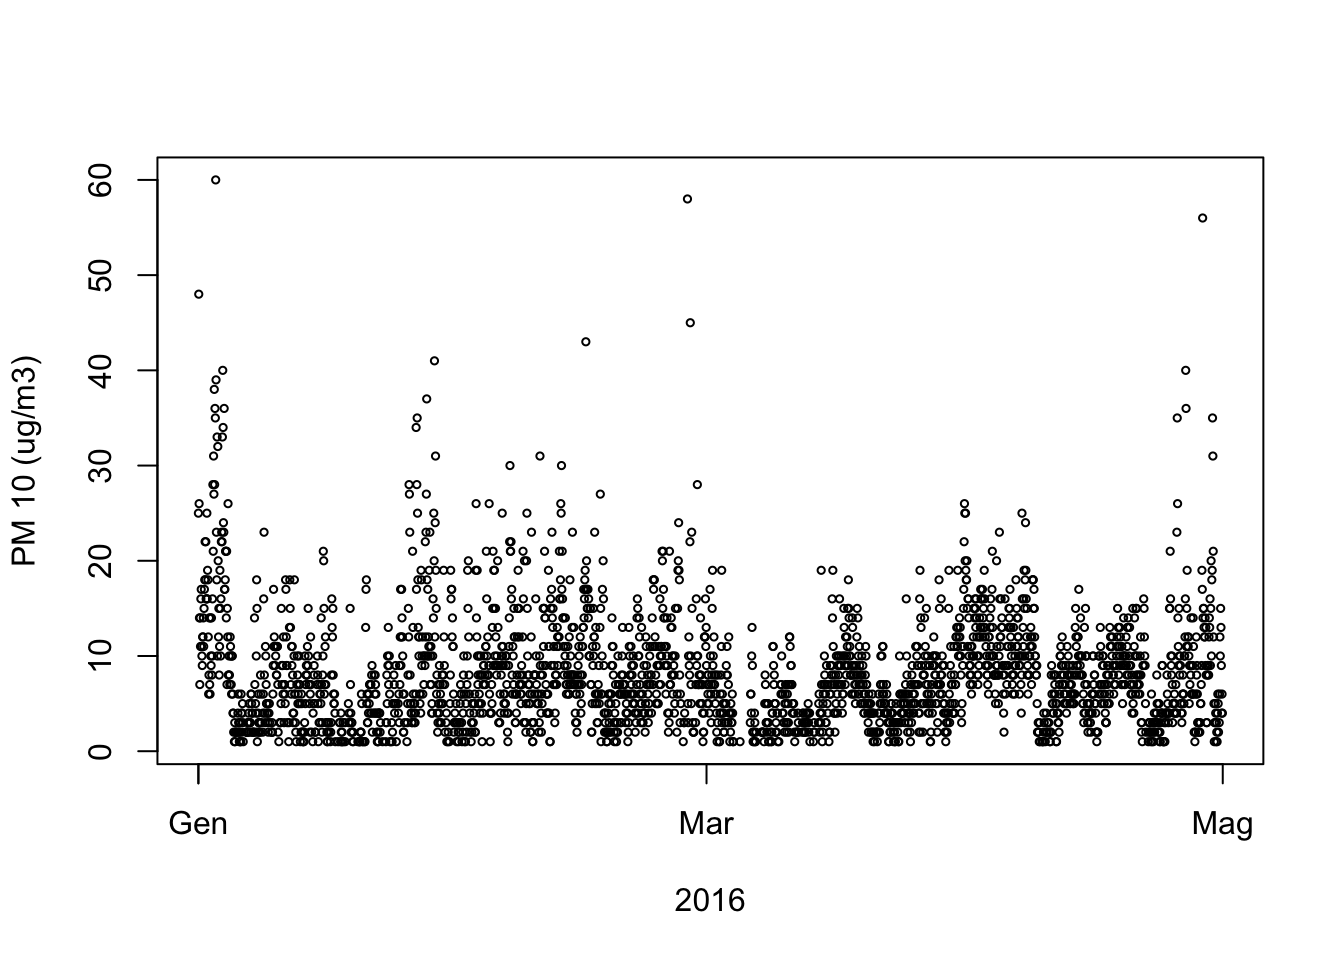
\includegraphics{bookdown_files/figure-latex/unnamed-chunk-71-1.pdf}

Poiché il grafico contiene un punto per ogni misurazione oraria, il grafico contiene moltissime informazioni.

Aggiungiamo una linea che indica il limite massimo giornaliero di PM 10 consentito (in Italia).

\begin{Shaded}
\begin{Highlighting}[]
\KeywordTok{plot}\NormalTok{(PM10dataSA}\OperatorTok{$}\NormalTok{DateTime.Local, PM10dataSA}\OperatorTok{$}\NormalTok{Sample.Measurement, }\DataTypeTok{xlab =} \StringTok{"2016"}\NormalTok{, }\DataTypeTok{ylab=} \StringTok{"PM 10 (ug/m3)"}\NormalTok{, }\DataTypeTok{cex =} \FloatTok{.5}\NormalTok{)}
\KeywordTok{abline}\NormalTok{(}\DataTypeTok{h =} \DecValTok{50}\NormalTok{, }\DataTypeTok{col =} \StringTok{"red"}\NormalTok{)}
\end{Highlighting}
\end{Shaded}

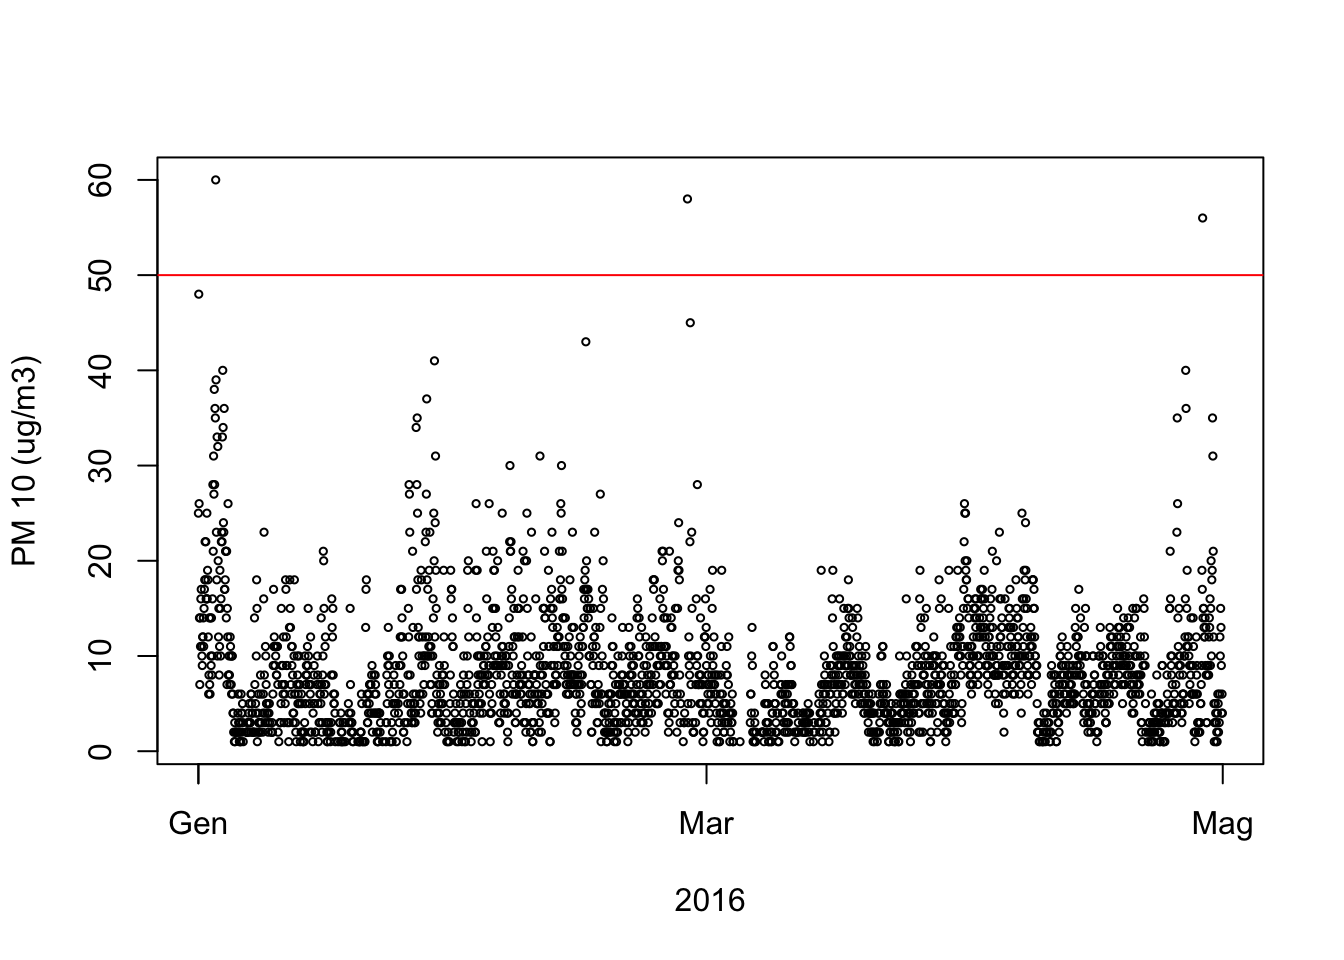
\includegraphics{bookdown_files/figure-latex/unnamed-chunk-72-1.pdf}

\begin{Shaded}
\begin{Highlighting}[]
\CommentTok{# Per salviare l'immagine}
\CommentTok{#png(filename="../plot/DailyPM10.png")}
\end{Highlighting}
\end{Shaded}

Si può notare che (fortunatamente) poche misurazioni superano i limiti consentiti.

\hypertarget{dati-giornalieri}{%
\subsection{Dati giornalieri}\label{dati-giornalieri}}

Vediamo di ridurle il numero di dati, aggregandoli per avere misurazioni giornaliere. Possiamo farlo usando la funzione \texttt{aggregate()} che ci permette di applicare una funzione ad un dataset indicando. Possiamo, ad esempio, decidere di salvare in un nuovo dataset le misure medie e massime per i dati di SA.

\begin{Shaded}
\begin{Highlighting}[]
\NormalTok{DailyVal <-}\StringTok{ }\KeywordTok{aggregate}\NormalTok{(PM10dataSA}\OperatorTok{$}\NormalTok{Sample.Measurement }\OperatorTok{~}\StringTok{ }\NormalTok{Date.Local, }\DataTypeTok{data =}\NormalTok{ PM10dataSA, }\DataTypeTok{FUN =}\NormalTok{ mean)}
\NormalTok{DailyVal[,}\DecValTok{3}\NormalTok{] <-}\StringTok{ }\KeywordTok{aggregate}\NormalTok{(PM10dataSA}\OperatorTok{$}\NormalTok{Sample.Measurement }\OperatorTok{~}\StringTok{ }\NormalTok{Date.Local, }\DataTypeTok{data =}\NormalTok{ PM10dataSA, }\DataTypeTok{FUN =}\NormalTok{ max)[}\DecValTok{2}\NormalTok{]}
\KeywordTok{head}\NormalTok{(DailyVal)}
\end{Highlighting}
\end{Shaded}

\begin{verbatim}
##   Date.Local PM10dataSA$Sample.Measurement PM10dataSA$Sample.Measurement.1
## 1 2016-01-01                      16.70833                              48
## 2 2016-01-02                      17.54167                              38
## 3 2016-01-03                      23.91667                              60
## 4 2016-01-04                      14.37500                              36
## 5 2016-01-05                       3.05000                              10
## 6 2016-01-06                       2.87500                               6
\end{verbatim}

Possiamo migliorare la leggibilità del dataset cambiando i nomi delle variabili.

\begin{Shaded}
\begin{Highlighting}[]
\KeywordTok{names}\NormalTok{(DailyVal)[}\DecValTok{2}\OperatorTok{:}\DecValTok{3}\NormalTok{] <-}\StringTok{ }\KeywordTok{c}\NormalTok{(}\StringTok{"mean daily PM10"}\NormalTok{, }\StringTok{"max daily PM 10"}\NormalTok{)}
\KeywordTok{head}\NormalTok{(DailyVal)}
\end{Highlighting}
\end{Shaded}

\begin{verbatim}
##   Date.Local mean daily PM10 max daily PM 10
## 1 2016-01-01        16.70833              48
## 2 2016-01-02        17.54167              38
## 3 2016-01-03        23.91667              60
## 4 2016-01-04        14.37500              36
## 5 2016-01-05         3.05000              10
## 6 2016-01-06         2.87500               6
\end{verbatim}

Visualizziamo ora i dati medi e massimi giornalieri:

\begin{Shaded}
\begin{Highlighting}[]
\KeywordTok{plot}\NormalTok{(DailyVal}\OperatorTok{$}\NormalTok{Date.Local, DailyVal}\OperatorTok{$}\StringTok{`}\DataTypeTok{mean daily PM10}\StringTok{`}\NormalTok{, }\DataTypeTok{xlab =} \StringTok{"2016"}\NormalTok{, }\DataTypeTok{ylab=} \StringTok{"PM 10 (ug/m3)"}\NormalTok{, }\DataTypeTok{cex =} \FloatTok{.8}\NormalTok{, }\DataTypeTok{main =} \StringTok{"Concentrazione media giornaliera di PM10"}\NormalTok{)}
\end{Highlighting}
\end{Shaded}

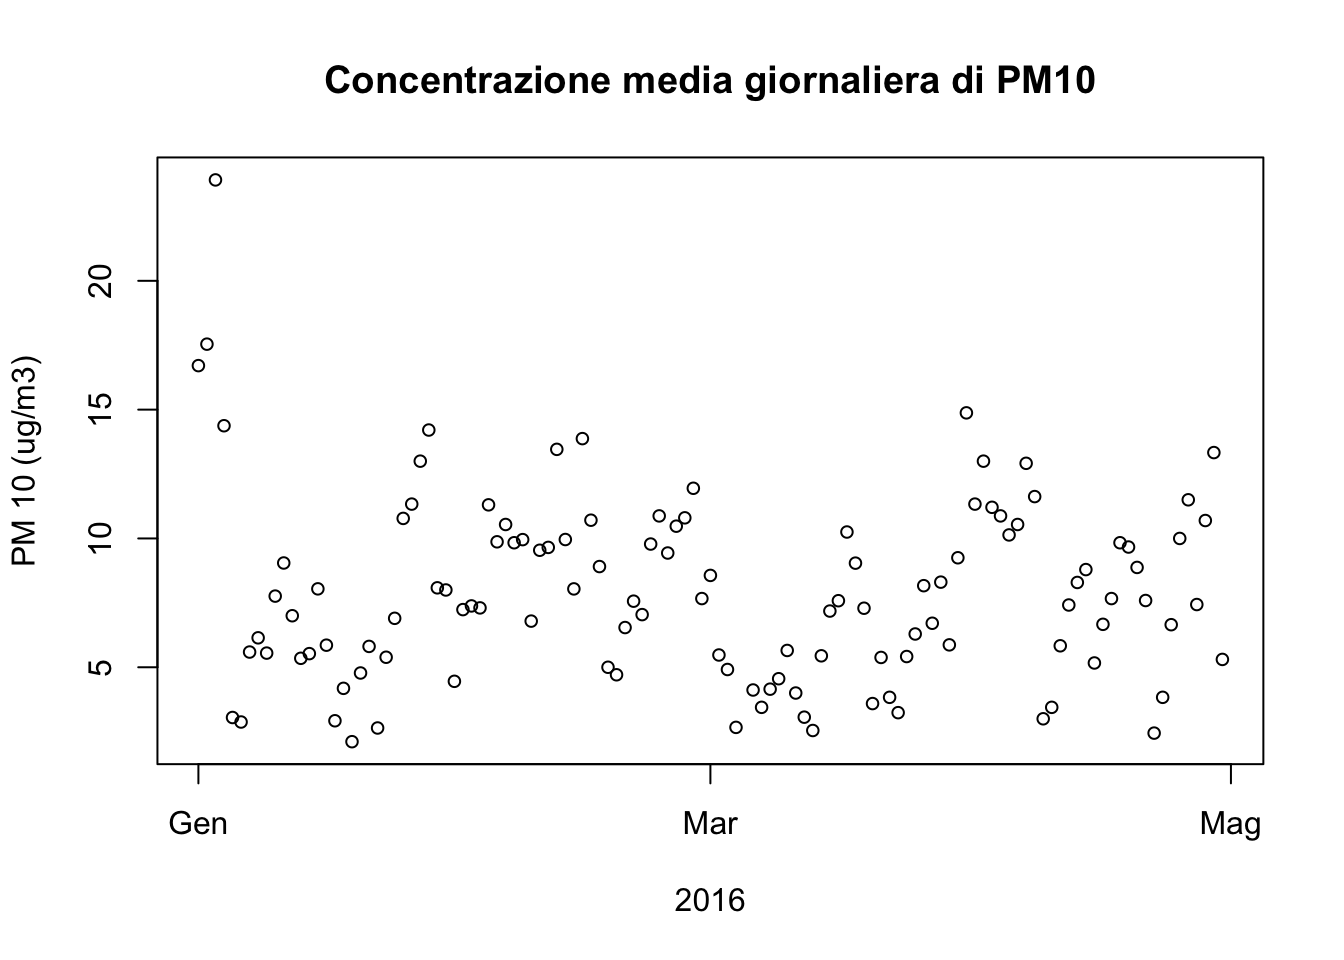
\includegraphics{bookdown_files/figure-latex/unnamed-chunk-75-1.pdf}

\begin{Shaded}
\begin{Highlighting}[]
\KeywordTok{plot}\NormalTok{(DailyVal}\OperatorTok{$}\NormalTok{Date.Local, DailyVal}\OperatorTok{$}\StringTok{`}\DataTypeTok{max daily PM 10}\StringTok{`}\NormalTok{, }\DataTypeTok{xlab =} \StringTok{"2016"}\NormalTok{, }\DataTypeTok{ylab=} \StringTok{"PM 10 (ug/m3)"}\NormalTok{, }\DataTypeTok{cex =} \FloatTok{.8}\NormalTok{, }\DataTypeTok{main =} \StringTok{"Concentrazione massima giornaliera di PM10"}\NormalTok{)}
\KeywordTok{abline}\NormalTok{(}\DataTypeTok{h =} \DecValTok{50}\NormalTok{, }\DataTypeTok{col =} \StringTok{"red"}\NormalTok{)}
\end{Highlighting}
\end{Shaded}

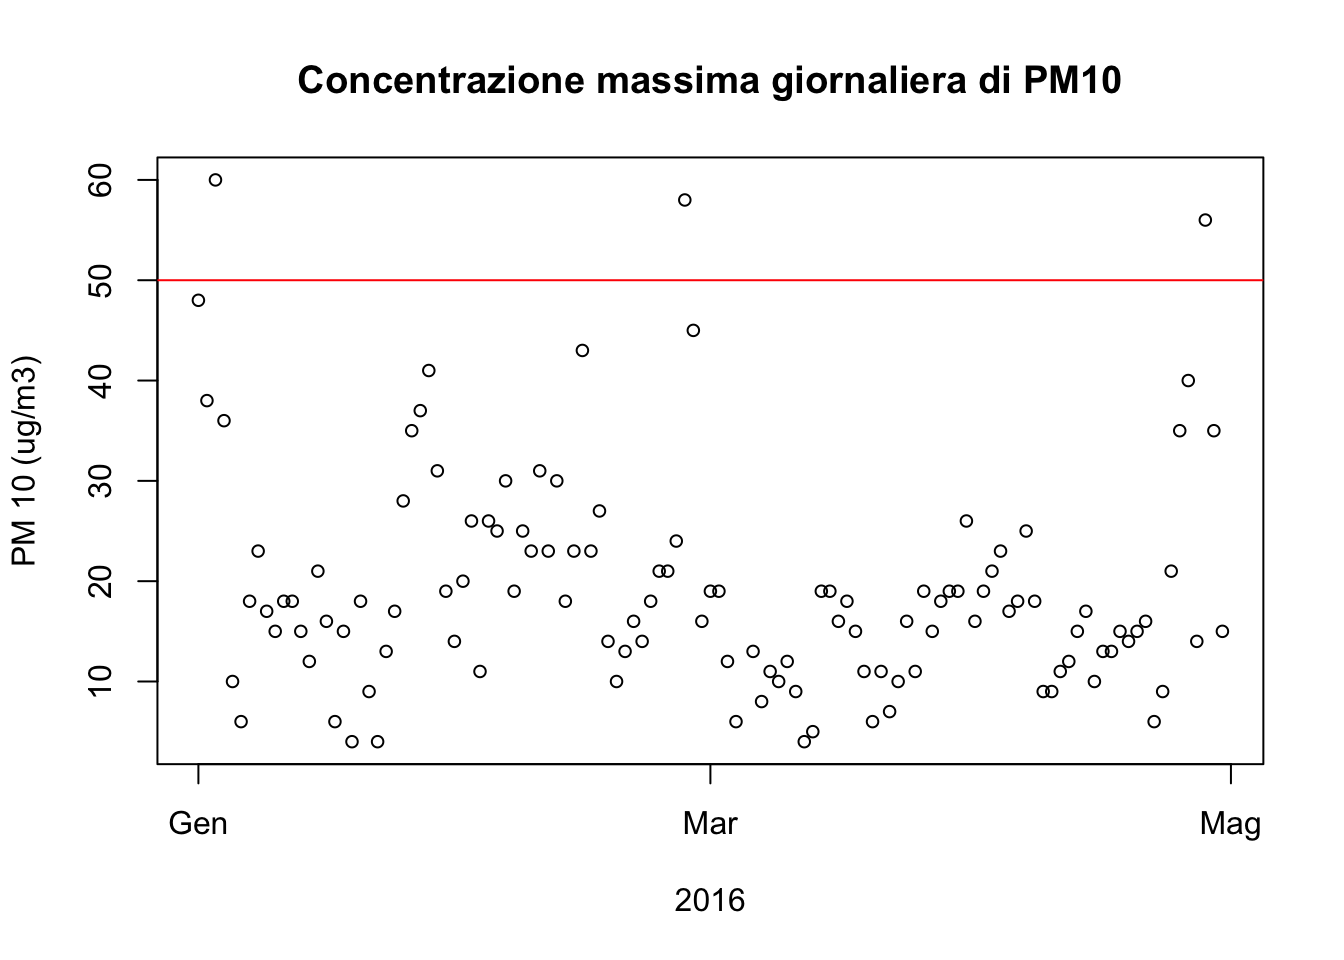
\includegraphics{bookdown_files/figure-latex/unnamed-chunk-76-1.pdf}

Potrebbe essere interessante vedere se il giorno della settimana influenza la concentrazione di PM10, ad esempio in giorni con più traffico potremmo aspettarci più inquinamento.

\begin{Shaded}
\begin{Highlighting}[]
\KeywordTok{typeof}\NormalTok{(DailyVal}\OperatorTok{$}\NormalTok{Date.Local)}
\end{Highlighting}
\end{Shaded}

\begin{verbatim}
## [1] "double"
\end{verbatim}

\begin{Shaded}
\begin{Highlighting}[]
\CommentTok{#Sys.setlocale("LC_TIME","C") #Nomi }
\NormalTok{DailyVal}\OperatorTok{$}\NormalTok{DayOfTheWeek <-}\StringTok{ }\KeywordTok{weekdays}\NormalTok{(DailyVal}\OperatorTok{$}\NormalTok{Date.Local, }\DataTypeTok{abbreviate =} \OtherTok{TRUE}\NormalTok{)}
\KeywordTok{head}\NormalTok{(DailyVal)}
\end{Highlighting}
\end{Shaded}

\begin{verbatim}
##   Date.Local mean daily PM10 max daily PM 10 DayOfTheWeek
## 1 2016-01-01        16.70833              48          Ven
## 2 2016-01-02        17.54167              38          Sab
## 3 2016-01-03        23.91667              60          Dom
## 4 2016-01-04        14.37500              36          Lun
## 5 2016-01-05         3.05000              10          Mar
## 6 2016-01-06         2.87500               6          Mer
\end{verbatim}

\begin{Shaded}
\begin{Highlighting}[]
\CommentTok{#ordiniamo i giorni in modo che la settimana inizi di lunedì}
\CommentTok{# ci sarà utile dopo}
\NormalTok{DailyVal}\OperatorTok{$}\NormalTok{DayOfTheWeek <-}\StringTok{ }\KeywordTok{ordered}\NormalTok{(DailyVal}\OperatorTok{$}\NormalTok{DayOfTheWeek, }\DataTypeTok{levels=}\KeywordTok{c}\NormalTok{( }\StringTok{"Lun"}\NormalTok{ , }\StringTok{"Mar"}\NormalTok{, }\StringTok{"Mer"}\NormalTok{ , }\StringTok{"Gio"}\NormalTok{, }\StringTok{"Ven"}\NormalTok{ ,  }\StringTok{"Sab"}\NormalTok{, }\StringTok{"Dom"}\NormalTok{ ))}
\end{Highlighting}
\end{Shaded}

Vediamo di colorare il grafico precedente usando un colore diverso per ogni giorno della settimana.

\begin{Shaded}
\begin{Highlighting}[]
\KeywordTok{plot}\NormalTok{(DailyVal}\OperatorTok{$}\NormalTok{Date.Local, DailyVal}\OperatorTok{$}\StringTok{`}\DataTypeTok{max daily PM 10}\StringTok{`}\NormalTok{, }\DataTypeTok{xlab =} \StringTok{"2016"}\NormalTok{, }\DataTypeTok{ylab=} \StringTok{"PM 10 (ug/m3)"}\NormalTok{, }\DataTypeTok{cex =} \FloatTok{.8}\NormalTok{, }\DataTypeTok{main =} \StringTok{"Concentrazione massima giornaliera di PM10"}\NormalTok{, }\DataTypeTok{col =}\NormalTok{ DailyVal}\OperatorTok{$}\NormalTok{DayOfTheWeek)}
\KeywordTok{abline}\NormalTok{(}\DataTypeTok{h =} \DecValTok{50}\NormalTok{, }\DataTypeTok{col =} \StringTok{"red"}\NormalTok{)}
\end{Highlighting}
\end{Shaded}

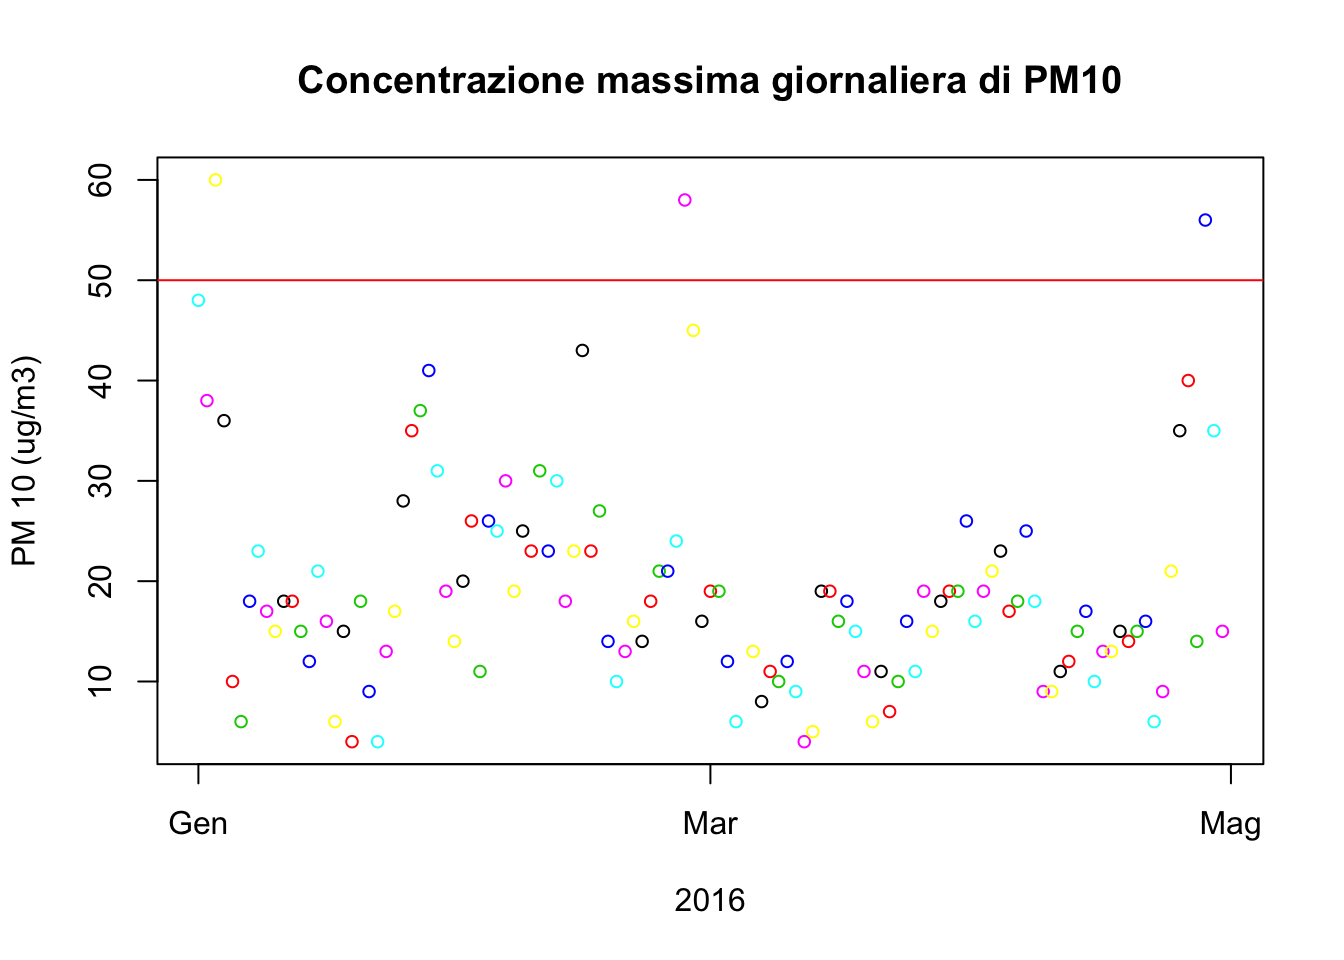
\includegraphics{bookdown_files/figure-latex/unnamed-chunk-78-1.pdf}

Vediamo che non sembra che i picchi siano raggiunti negli stessi giorni. Comunque una legenda andrebbe aggiunta. Vediamo con dei boxplot come la quantità media di polveri PM10 è distribuita rispetto ai giorni della settimana.

\begin{Shaded}
\begin{Highlighting}[]
\KeywordTok{boxplot}\NormalTok{(}\StringTok{`}\DataTypeTok{mean daily PM10}\StringTok{`} \OperatorTok{~}\StringTok{ }\NormalTok{DayOfTheWeek, }\DataTypeTok{data =}\NormalTok{ DailyVal, }\DataTypeTok{ylab=} \StringTok{"PM 10 (ug/m3)"}\NormalTok{)}
\end{Highlighting}
\end{Shaded}

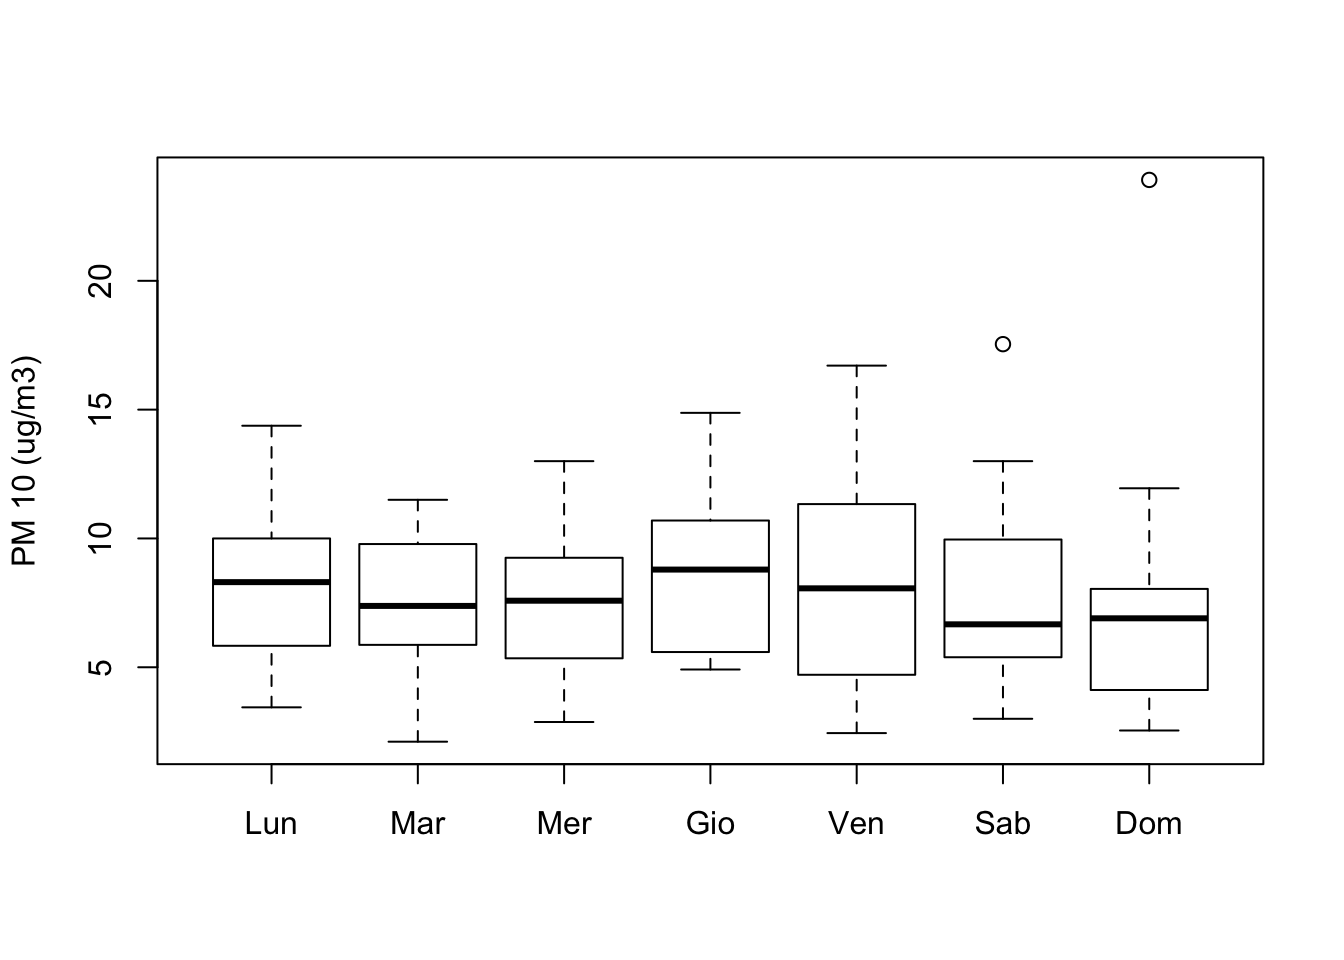
\includegraphics{bookdown_files/figure-latex/unnamed-chunk-79-1.pdf}

Aggiungere ad esempio una linea che indica le media delle misurazioni, aiuta a fare un confronto tra i dati.

\begin{Shaded}
\begin{Highlighting}[]
\KeywordTok{boxplot}\NormalTok{( }\StringTok{`}\DataTypeTok{mean daily PM10}\StringTok{`} \OperatorTok{~}\StringTok{ }\NormalTok{DayOfTheWeek, }\DataTypeTok{data =}\NormalTok{ DailyVal, }\DataTypeTok{ylab=} \StringTok{"PM 10 (ug/m3)"}\NormalTok{)}
\KeywordTok{abline}\NormalTok{(}\DataTypeTok{h =} \KeywordTok{mean}\NormalTok{(DailyVal}\OperatorTok{$}\StringTok{`}\DataTypeTok{mean daily PM10}\StringTok{`}\NormalTok{), }\DataTypeTok{col =} \StringTok{"red"}\NormalTok{)}
\end{Highlighting}
\end{Shaded}

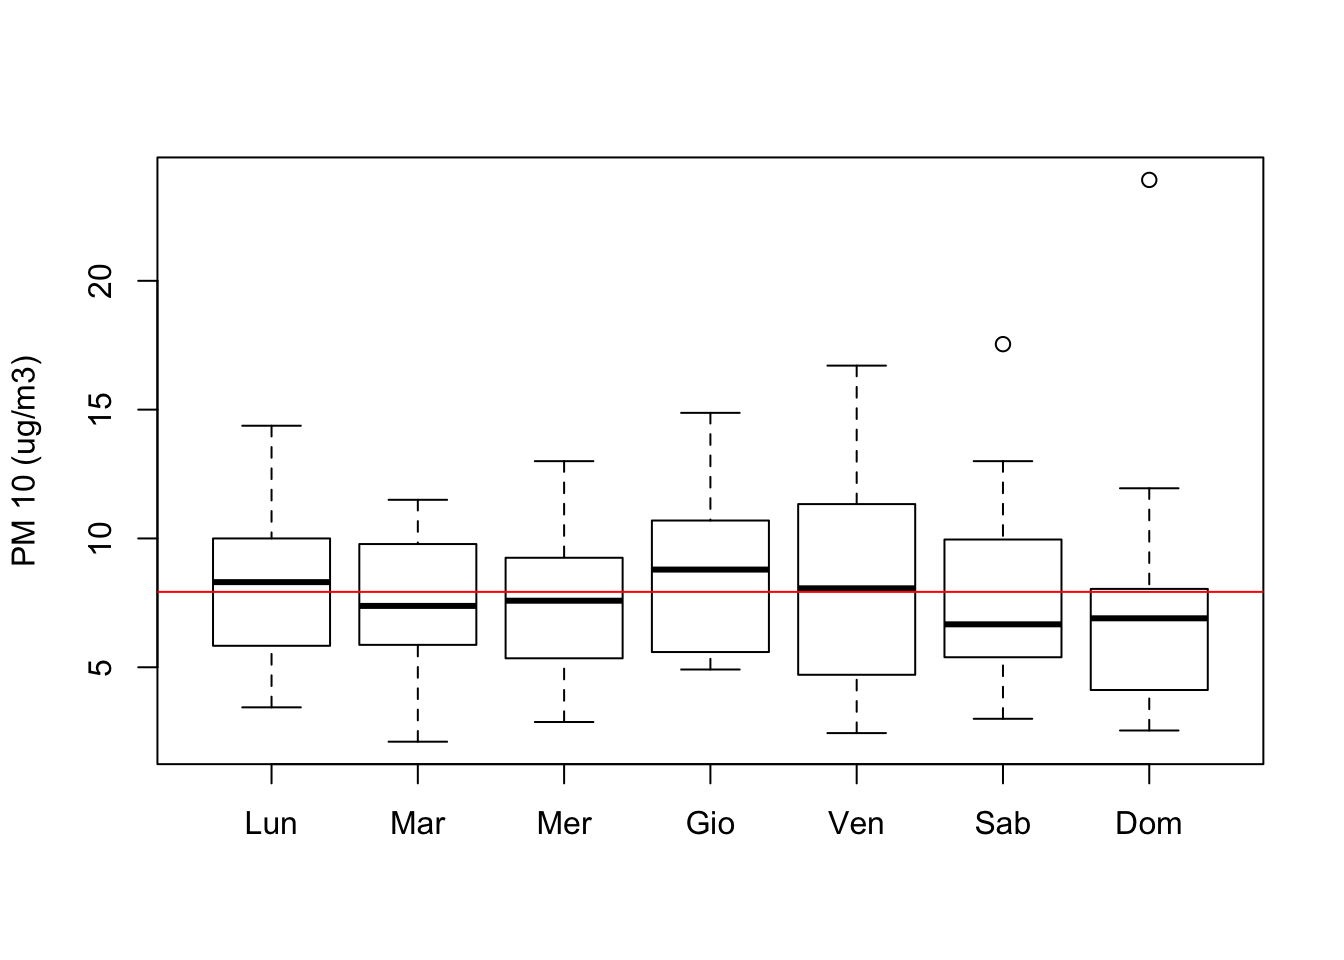
\includegraphics{bookdown_files/figure-latex/unnamed-chunk-80-1.pdf}

Vediamo la data in cui è stato assunto il valore massimo:

\begin{Shaded}
\begin{Highlighting}[]
\NormalTok{DailyVal[DailyVal}\OperatorTok{$}\StringTok{`}\DataTypeTok{mean daily PM10}\StringTok{`} \OperatorTok{>}\StringTok{ }\DecValTok{20}\NormalTok{,]}
\end{Highlighting}
\end{Shaded}

\begin{verbatim}
##   Date.Local mean daily PM10 max daily PM 10 DayOfTheWeek
## 3 2016-01-03        23.91667              60          Dom
\end{verbatim}

Che sarà successo quel giorno? Potrebbe essere un errore di lettura?

Se volessimo visualizzare la distribuzione dei dati rispetto ai giorni, possiamo usare la funzione \texttt{hist()}. Purtroppo tale funzione non supporta la notazione \texttt{\textasciitilde{}}, perciò dovremo specificare un grafico per giorno della settimana.

\begin{Shaded}
\begin{Highlighting}[]
\KeywordTok{par}\NormalTok{(}\DataTypeTok{mfrow =} \KeywordTok{c}\NormalTok{(}\DecValTok{7}\NormalTok{,}\DecValTok{1}\NormalTok{), }\DataTypeTok{mar =} \KeywordTok{c}\NormalTok{(}\DecValTok{2}\NormalTok{,}\DecValTok{2}\NormalTok{,}\DecValTok{1}\NormalTok{,}\DecValTok{1}\NormalTok{))}
\ControlFlowTok{for}\NormalTok{ (i }\ControlFlowTok{in} \KeywordTok{levels}\NormalTok{(DailyVal}\OperatorTok{$}\NormalTok{DayOfTheWeek) ) \{}
  \KeywordTok{hist}\NormalTok{( DailyVal[DailyVal}\OperatorTok{$}\NormalTok{DayOfTheWeek }\OperatorTok{==}\StringTok{ }\NormalTok{i, }\StringTok{"mean daily PM10"}\NormalTok{] , }\DataTypeTok{freq =} \OtherTok{FALSE}\NormalTok{, }\DataTypeTok{main =}\NormalTok{ i, }\DataTypeTok{ylim =} \KeywordTok{c}\NormalTok{(}\DecValTok{0}\NormalTok{, }\FloatTok{0.2}\NormalTok{) , }\DataTypeTok{breaks =} \KeywordTok{seq}\NormalTok{(}\DecValTok{0}\NormalTok{,}\DecValTok{26}\NormalTok{,}\DecValTok{2}\NormalTok{))}
\NormalTok{\}}
\end{Highlighting}
\end{Shaded}

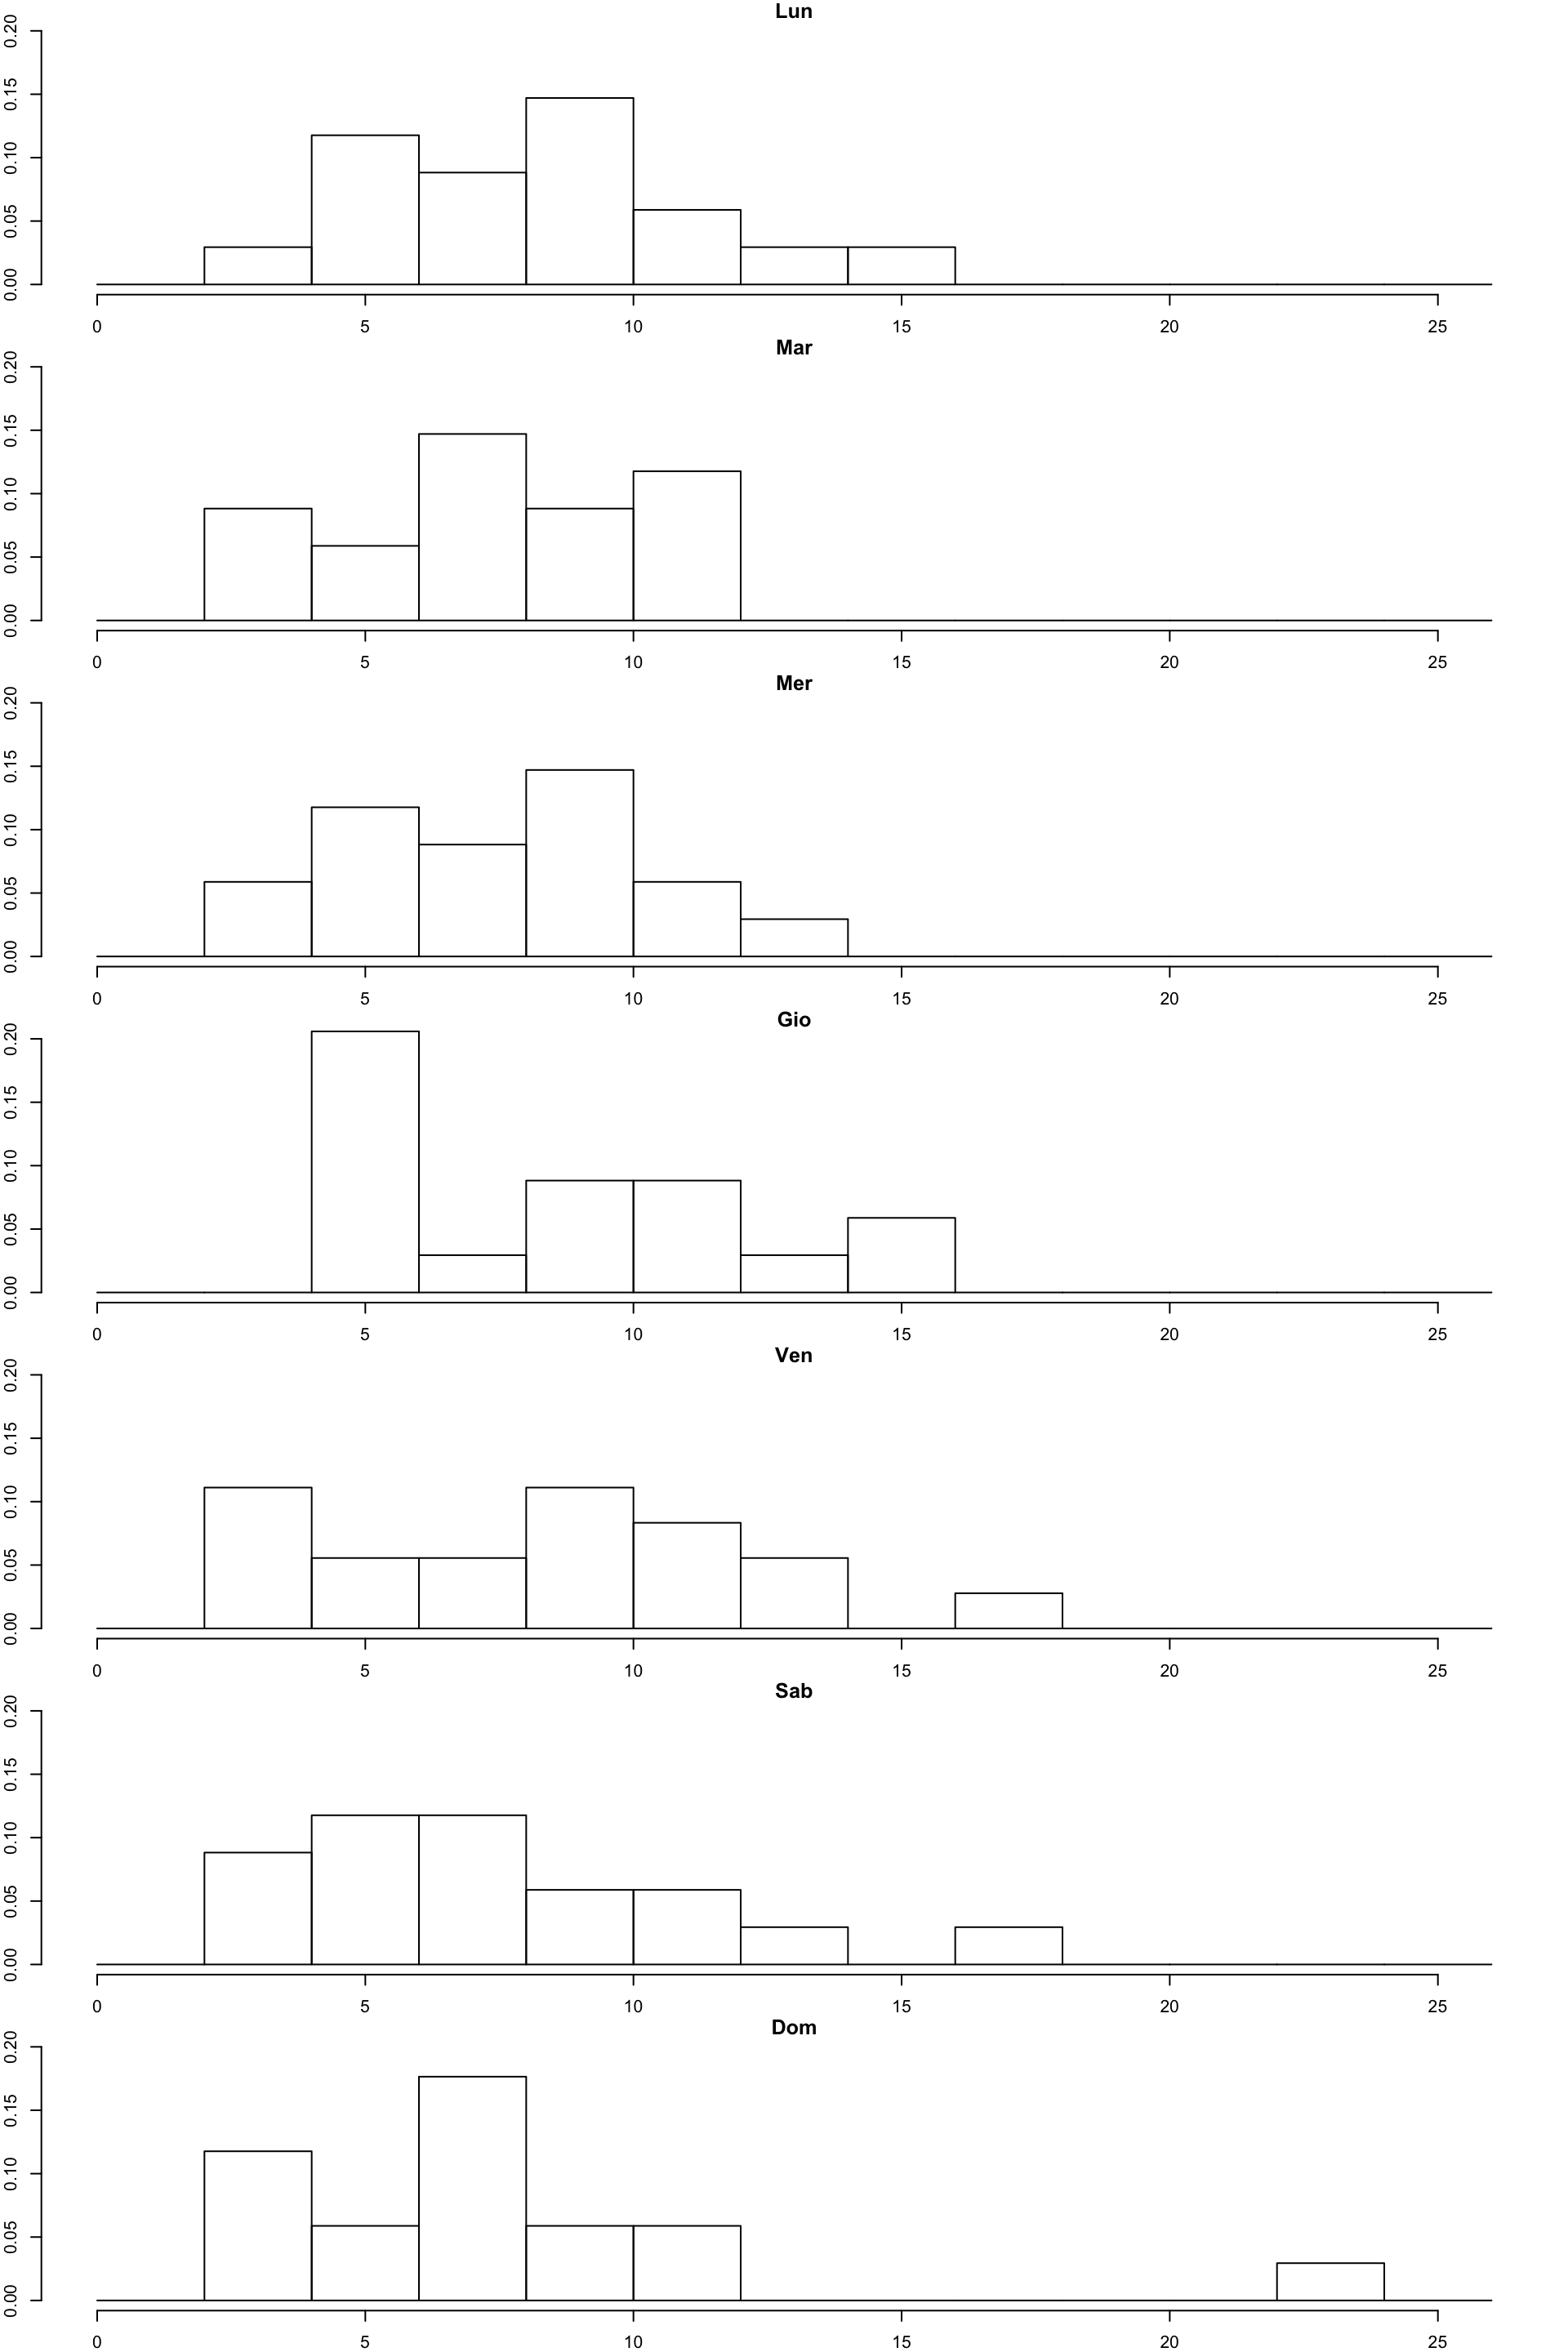
\includegraphics{bookdown_files/figure-latex/unnamed-chunk-82-1.pdf}

Dal grafico possiamo capire come si distribuiscono le misurazioni rispetto ai giorni della settimana.
Si usi l'help per comprendere i parametri che sono stati usati.

\hypertarget{inquinamento-in-california}{%
\section{Inquinamento in California}\label{inquinamento-in-california}}

Decidiamo ora di concentrare la nostra attenzione sull'inquinamento in California e dopo aver letto il \href{https://www.dropbox.com/s/z926dmp2lvdz48p/daily_81102_2016.csv?dl=1}{dataset} che contiene i valori \textbf{medi giornalieri} di PM10, salviamo un sottoinsieme di dati che contiene solo dati relativi alla California.

\begin{Shaded}
\begin{Highlighting}[]
\NormalTok{PM10data <-}\StringTok{ }\KeywordTok{read.csv}\NormalTok{(}\StringTok{"./data/daily_81102_2016.csv"}\NormalTok{)}
\KeywordTok{dim}\NormalTok{(PM10data)}
\end{Highlighting}
\end{Shaded}

\begin{verbatim}
## [1] 118885     29
\end{verbatim}

Vediamo che il file è molto grande, contiene molte righe e molte variabili. R impiega diverso tempo a leggerlo.

\begin{Shaded}
\begin{Highlighting}[]
\NormalTok{PM10dataCAL <-}\StringTok{ }\NormalTok{PM10data[PM10data}\OperatorTok{$}\NormalTok{State.Name }\OperatorTok{==}\StringTok{ "California"}\NormalTok{,]}
\NormalTok{knitr}\OperatorTok{::}\KeywordTok{kable}\NormalTok{(}
\KeywordTok{head}\NormalTok{(PM10dataCAL),}
\DataTypeTok{booktabs =} \OtherTok{TRUE}
\NormalTok{)}
\end{Highlighting}
\end{Shaded}

\begin{tabular}{lrrrrrrrlllllllrrrrrrrllllllll}
\toprule
  & State.Code & County.Code & Site.Num & Parameter.Code & POC & Latitude & Longitude & Datum & Parameter.Name & Sample.Duration & Pollutant.Standard & Date.Local & Units.of.Measure & Event.Type & Observation.Count & Observation.Percent & Arithmetic.Mean & X1st.Max.Value & X1st.Max.Hour & AQI & Method.Code & Method.Name & Local.Site.Name & Address & State.Name & County.Name & City.Name & CBSA.Name & Date.of.Last.Change\\
\midrule
15472 & 6 & 7 & 8 & 81102 & 3 & 39.76154 & -121.8416 & WGS84 & PM10 Total 0-10um STP & 24-HR BLK AVG & PM10 24-hour 2006 & 2016-01-01 & Micrograms/cubic meter (25 C) & None & 1 & 100 & 21 & 21 & 23 & 19 & NA & - & Chico-East Avenue & 984 East Avenue, Chico & California & Butte & Chico & Chico, CA & 2016-11-08\\
15473 & 6 & 7 & 8 & 81102 & 3 & 39.76154 & -121.8416 & WGS84 & PM10 Total 0-10um STP & 24-HR BLK AVG & PM10 24-hour 2006 & 2016-01-02 & Micrograms/cubic meter (25 C) & None & 1 & 100 & 18 & 18 & 23 & 17 & NA & - & Chico-East Avenue & 984 East Avenue, Chico & California & Butte & Chico & Chico, CA & 2016-11-08\\
15474 & 6 & 7 & 8 & 81102 & 3 & 39.76154 & -121.8416 & WGS84 & PM10 Total 0-10um STP & 24-HR BLK AVG & PM10 24-hour 2006 & 2016-01-03 & Micrograms/cubic meter (25 C) & None & 1 & 100 & 23 & 23 & 23 & 21 & NA & - & Chico-East Avenue & 984 East Avenue, Chico & California & Butte & Chico & Chico, CA & 2016-11-08\\
15475 & 6 & 7 & 8 & 81102 & 3 & 39.76154 & -121.8416 & WGS84 & PM10 Total 0-10um STP & 24-HR BLK AVG & PM10 24-hour 2006 & 2016-01-04 & Micrograms/cubic meter (25 C) & None & 1 & 100 & 31 & 31 & 23 & 29 & NA & - & Chico-East Avenue & 984 East Avenue, Chico & California & Butte & Chico & Chico, CA & 2016-11-08\\
15476 & 6 & 7 & 8 & 81102 & 3 & 39.76154 & -121.8416 & WGS84 & PM10 Total 0-10um STP & 24-HR BLK AVG & PM10 24-hour 2006 & 2016-01-05 & Micrograms/cubic meter (25 C) & None & 1 & 100 & 9 & 9 & 23 & 8 & NA & - & Chico-East Avenue & 984 East Avenue, Chico & California & Butte & Chico & Chico, CA & 2016-11-08\\
\addlinespace
15477 & 6 & 7 & 8 & 81102 & 3 & 39.76154 & -121.8416 & WGS84 & PM10 Total 0-10um STP & 24-HR BLK AVG & PM10 24-hour 2006 & 2016-01-06 & Micrograms/cubic meter (25 C) & None & 1 & 100 & 6 & 6 & 23 & 6 & NA & - & Chico-East Avenue & 984 East Avenue, Chico & California & Butte & Chico & Chico, CA & 2016-11-08\\
\bottomrule
\end{tabular}

In questo caso il nome della variabile che ci interessa è \emph{Arithmetic.Mean}.

Ora vogliamo visualizzare su una mappa quali sono lo città che superano la soglia di inquinamento consentita durante le osservazioni. In R, questa operazione è molto semplice usando i pacchetti \texttt{maps} o \texttt{RgoogleMaps}.

\begin{Shaded}
\begin{Highlighting}[]
\CommentTok{#install.packages("maps")}
\KeywordTok{library}\NormalTok{(maps)}
\KeywordTok{map}\NormalTok{(}\StringTok{"county"}\NormalTok{, }\StringTok{"california"}\NormalTok{, }\DataTypeTok{xlim=}\KeywordTok{c}\NormalTok{(}\OperatorTok{-}\DecValTok{125}\NormalTok{,}\OperatorTok{-}\DecValTok{114}\NormalTok{), }\DataTypeTok{ylim=}\KeywordTok{c}\NormalTok{(}\DecValTok{32}\NormalTok{,}\DecValTok{43}\NormalTok{))}
\KeywordTok{points}\NormalTok{( PM10dataCAL[PM10dataCAL}\OperatorTok{$}\NormalTok{Arithmetic.Mean }\OperatorTok{>}\StringTok{ }\DecValTok{50}\NormalTok{,}\KeywordTok{c}\NormalTok{(}\StringTok{"Longitude"}\NormalTok{, }\StringTok{"Latitude"}\NormalTok{)] ,}\DataTypeTok{cex =} \FloatTok{.8}\NormalTok{, }\DataTypeTok{col =} \StringTok{"red"}\NormalTok{)}
\end{Highlighting}
\end{Shaded}

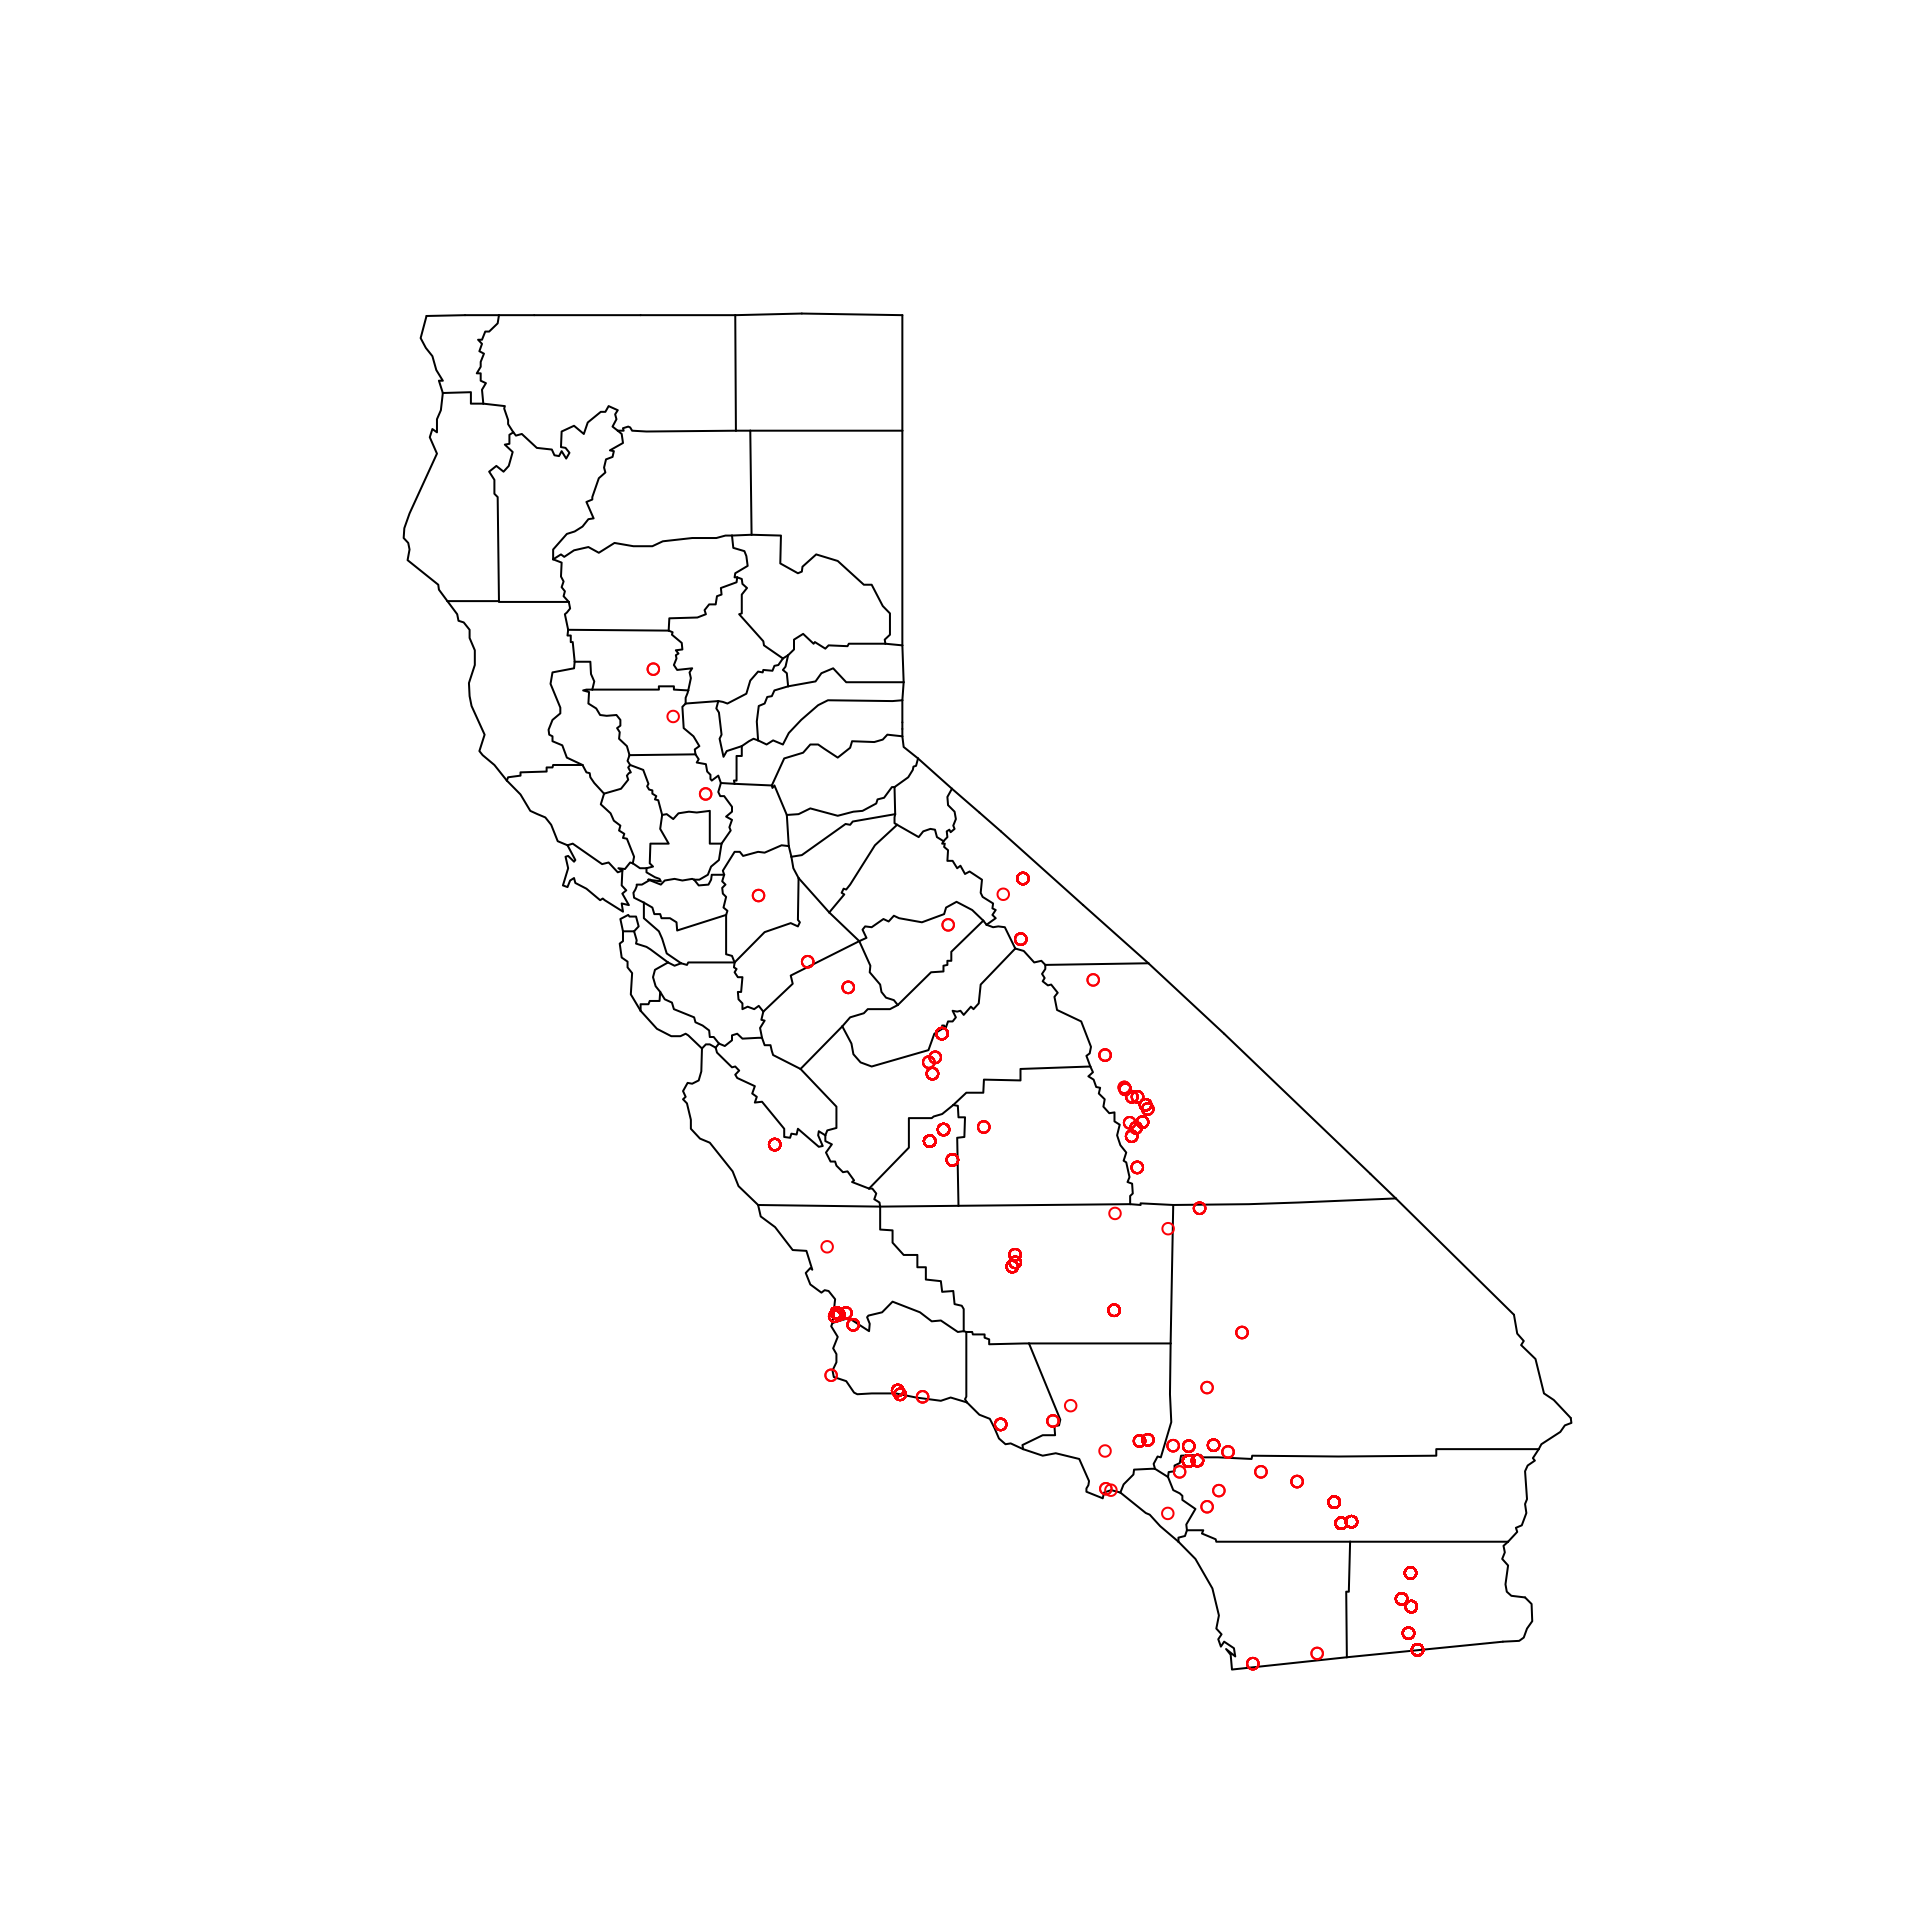
\includegraphics{bookdown_files/figure-latex/unnamed-chunk-85-1.pdf}

\hypertarget{inquinamento-a-los-angeles}{%
\section{Inquinamento a Los Angeles}\label{inquinamento-a-los-angeles}}

Usiamo lo stesso dataset contenente i dati giornalieri relativi alle PM10 negli Stati Uniti e concentriamoci sulla sola città di Los Angeles.

\begin{Shaded}
\begin{Highlighting}[]
\NormalTok{PM10dataLA <-}\StringTok{ }\NormalTok{PM10data[PM10data}\OperatorTok{$}\NormalTok{City.Name}\OperatorTok{==}\StringTok{ "Los Angeles"}\NormalTok{,]}
\KeywordTok{dim}\NormalTok{(PM10dataLA)}
\end{Highlighting}
\end{Shaded}

\begin{verbatim}
## [1] 90 29
\end{verbatim}

Vediamo che sono state raccolte 90 osservazioni relative alla sola città di LA, cerchiamo di capire quando e con che frequenza sono state raccolte.

\begin{Shaded}
\begin{Highlighting}[]
\KeywordTok{typeof}\NormalTok{(PM10dataLA)}
\end{Highlighting}
\end{Shaded}

\begin{verbatim}
## [1] "list"
\end{verbatim}

\begin{Shaded}
\begin{Highlighting}[]
\NormalTok{PM10dataLA}\OperatorTok{$}\NormalTok{Date.Local[}\DecValTok{1}\OperatorTok{:}\DecValTok{10}\NormalTok{]}
\end{Highlighting}
\end{Shaded}

\begin{verbatim}
##  [1] 2016-01-01 2016-01-07 2016-01-13 2016-01-19 2016-01-25 2016-01-31
##  [7] 2016-02-06 2016-02-12 2016-02-18 2016-02-24
## 336 Levels: 2016-01-01 2016-01-02 2016-01-03 2016-01-04 ... 2016-12-02
\end{verbatim}

Vediamo che le date sono state salvate come liste. In realtà, come già visto, R prevede il formato \emph{Date} che potrebbe essere utile e più maneggevole di una lista per fare ``operazioni aritmetiche''. Convertiamo quindi la colonna in \emph{Date}.

\begin{Shaded}
\begin{Highlighting}[]
\NormalTok{PM10dataLA}\OperatorTok{$}\NormalTok{Date.Local <-}\StringTok{ }\KeywordTok{as.Date}\NormalTok{(PM10dataLA}\OperatorTok{$}\NormalTok{Date.Local)}
\KeywordTok{typeof}\NormalTok{(PM10dataLA}\OperatorTok{$}\NormalTok{Date.Local)}
\end{Highlighting}
\end{Shaded}

\begin{verbatim}
## [1] "double"
\end{verbatim}

La variabile ora risulta di tipo \emph{Date.} Questo ci permette, ad esempio, di vedere quanti giorni passano tra una rilevazione e l'altra.

\begin{Shaded}
\begin{Highlighting}[]
\KeywordTok{diff}\NormalTok{(PM10dataLA}\OperatorTok{$}\NormalTok{Date.Local)}
\end{Highlighting}
\end{Shaded}

\begin{verbatim}
## Time differences in days
##  [1]    6    6    6    6    6    6    6    6    6    6    6    6    6    6
## [15]    6    6    6    6    6    6    7    5    6    6    6    6    6    6
## [29]    6    6    6    6    6    6    6    6    6    6    6    6    6    6
## [43]    6   12 -270    6    6    6    6    6    6    6    6    6    6    6
## [57]    6    6   12    6    6    6    6    6    6    6    6    6    6    6
## [71]    6    6    6    6    6    6    6    6    6    6    6    6    6    6
## [85]    6    6    6    6    6
\end{verbatim}

Salta all'occhio che la frequenza delle registrazioni è circa ogni 6 giorni, ma compare un dato inatteso. Investighiamo meglio cosa è successo.

\begin{Shaded}
\begin{Highlighting}[]
\KeywordTok{unique}\NormalTok{(PM10dataLA}\OperatorTok{$}\NormalTok{Date.Local)}
\end{Highlighting}
\end{Shaded}

\begin{verbatim}
##  [1] "2016-01-01" "2016-01-07" "2016-01-13" "2016-01-19" "2016-01-25"
##  [6] "2016-01-31" "2016-02-06" "2016-02-12" "2016-02-18" "2016-02-24"
## [11] "2016-03-01" "2016-03-07" "2016-03-13" "2016-03-19" "2016-03-25"
## [16] "2016-03-31" "2016-04-06" "2016-04-12" "2016-04-18" "2016-04-24"
## [21] "2016-04-30" "2016-05-07" "2016-05-12" "2016-05-18" "2016-05-24"
## [26] "2016-05-30" "2016-06-05" "2016-06-11" "2016-06-17" "2016-06-23"
## [31] "2016-06-29" "2016-07-05" "2016-07-11" "2016-07-17" "2016-07-23"
## [36] "2016-07-29" "2016-08-04" "2016-08-10" "2016-08-16" "2016-08-22"
## [41] "2016-08-28" "2016-09-03" "2016-09-09" "2016-09-15" "2016-09-27"
## [46] "2016-05-06" "2016-09-21"
\end{verbatim}

\begin{Shaded}
\begin{Highlighting}[]
\KeywordTok{length}\NormalTok{(}\KeywordTok{unique}\NormalTok{(PM10dataLA}\OperatorTok{$}\NormalTok{Date.Local))}
\end{Highlighting}
\end{Shaded}

\begin{verbatim}
## [1] 47
\end{verbatim}

Capiamo che sebbene le osservazioni siano 90, non tutte si riferiscono a giorni differenti, quindi bisogna capire come gestire le misurazioni ripetute durante lo stesso giorno. Vediamo, ad esempio, cosa caratterizza le misurazioni ripetute del primo giorno dell'anno.

\begin{Shaded}
\begin{Highlighting}[]
\NormalTok{PM10dataLA[PM10dataLA}\OperatorTok{$}\NormalTok{Date.Local}\OperatorTok{==}\StringTok{ "2016-01-01"}\NormalTok{,]}
\end{Highlighting}
\end{Shaded}

\begin{verbatim}
##       State.Code County.Code Site.Num Parameter.Code POC Latitude
## 23477          6          37     1103          81102   2 34.06659
## 23613          6          37     5005          81102   1 33.95080
##       Longitude Datum        Parameter.Name Sample.Duration
## 23477 -118.2269 WGS84 PM10 Total 0-10um STP         24 HOUR
## 23613 -118.4304 WGS84 PM10 Total 0-10um STP         24 HOUR
##       Pollutant.Standard Date.Local              Units.of.Measure
## 23477  PM10 24-hour 2006 2016-01-01 Micrograms/cubic meter (25 C)
## 23613  PM10 24-hour 2006 2016-01-01 Micrograms/cubic meter (25 C)
##       Event.Type Observation.Count Observation.Percent Arithmetic.Mean
## 23477       None                 1                 100              17
## 23613       None                 1                 100              12
##       X1st.Max.Value X1st.Max.Hour AQI Method.Code
## 23477             17             0  16          63
## 23613             12             0  11          63
##                            Method.Name               Local.Site.Name
## 23477 HI-VOL SA/GMW-1200 - GRAVIMETRIC Los Angeles-North Main Street
## 23613 HI-VOL SA/GMW-1200 - GRAVIMETRIC                  LAX Hastings
##                           Address State.Name County.Name   City.Name
## 23477 1630 N MAIN ST, LOS ANGELES California Los Angeles Los Angeles
## 23613 7201 W. WESTCHESTER PARKWAY California Los Angeles Los Angeles
##                                CBSA.Name Date.of.Last.Change
## 23477 Los Angeles-Long Beach-Anaheim, CA          2016-12-20
## 23613 Los Angeles-Long Beach-Anaheim, CA          2016-12-20
\end{verbatim}

Possiamo osservare che ci sono almeno due siti diversi dove vengono raccolti i dati. Questa osservazione segue sia la comparsa di due diversi \emph{Site.Num} per la stessa data, sia le differenze nei valori di \emph{Latitude} e \emph{Longitude}. Vediamo se esistono solo due siti o più.

\begin{Shaded}
\begin{Highlighting}[]
\KeywordTok{paste}\NormalTok{(}\KeywordTok{unique}\NormalTok{(PM10dataLA}\OperatorTok{$}\NormalTok{Site.Num) , }\KeywordTok{unique}\NormalTok{(PM10dataLA}\OperatorTok{$}\NormalTok{Latitude), }\KeywordTok{unique}\NormalTok{(PM10dataLA}\OperatorTok{$}\NormalTok{Longitude))}
\end{Highlighting}
\end{Shaded}

\begin{verbatim}
## [1] "1103 34.06659 -118.22688" "5005 33.9508 -118.43043"
\end{verbatim}

Abbiamo appurato che esistono due (e solo due) siti individuati da diverse coordinate geografiche.

Estrapoliamo ora alcune informazioni per le variabili numeriche usando il comando \texttt{summary()}.

\begin{Shaded}
\begin{Highlighting}[]
\KeywordTok{summary}\NormalTok{(PM10dataLA)}
\end{Highlighting}
\end{Shaded}

\begin{verbatim}
##    State.Code  County.Code    Site.Num    Parameter.Code       POC     
##  Min.   :6    Min.   :37   Min.   :1103   Min.   :81102   Min.   :1.0  
##  1st Qu.:6    1st Qu.:37   1st Qu.:1103   1st Qu.:81102   1st Qu.:1.0  
##  Median :6    Median :37   Median :3054   Median :81102   Median :1.5  
##  Mean   :6    Mean   :37   Mean   :3054   Mean   :81102   Mean   :1.5  
##  3rd Qu.:6    3rd Qu.:37   3rd Qu.:5005   3rd Qu.:81102   3rd Qu.:2.0  
##  Max.   :6    Max.   :37   Max.   :5005   Max.   :81102   Max.   :2.0  
##                                                                        
##     Latitude       Longitude        Datum                  Parameter.Name
##  Min.   :33.95   Min.   :-118.4   NAD83: 0   PM10 Total 0-10um STP:90    
##  1st Qu.:33.95   1st Qu.:-118.4   WGS84:90                               
##  Median :34.01   Median :-118.3                                          
##  Mean   :34.01   Mean   :-118.3                                          
##  3rd Qu.:34.07   3rd Qu.:-118.2                                          
##  Max.   :34.07   Max.   :-118.2                                          
##                                                                          
##       Sample.Duration         Pollutant.Standard   Date.Local        
##  24 HOUR      :90     PM10 24-hour 2006:90       Min.   :2016-01-01  
##  24-HR BLK AVG: 0                                1st Qu.:2016-03-07  
##                                                  Median :2016-05-15  
##                                                  Mean   :2016-05-14  
##                                                  3rd Qu.:2016-07-21  
##                                                  Max.   :2016-09-27  
##                                                                      
##                       Units.of.Measure    Event.Type Observation.Count
##  Micrograms/cubic meter (25 C):90      Excluded: 0   Min.   :1        
##                                        Included: 0   1st Qu.:1        
##                                        None    :90   Median :1        
##                                                      Mean   :1        
##                                                      3rd Qu.:1        
##                                                      Max.   :1        
##                                                                       
##  Observation.Percent Arithmetic.Mean X1st.Max.Value  X1st.Max.Hour
##  Min.   :100         Min.   : 6.00   Min.   : 6.00   Min.   :0    
##  1st Qu.:100         1st Qu.:16.00   1st Qu.:16.00   1st Qu.:0    
##  Median :100         Median :20.50   Median :20.50   Median :0    
##  Mean   :100         Mean   :22.18   Mean   :22.18   Mean   :0    
##  3rd Qu.:100         3rd Qu.:28.00   3rd Qu.:28.00   3rd Qu.:0    
##  Max.   :100         Max.   :57.00   Max.   :57.00   Max.   :0    
##                                                                   
##       AQI         Method.Code
##  Min.   : 6.00   Min.   :63  
##  1st Qu.:15.00   1st Qu.:63  
##  Median :19.00   Median :63  
##  Mean   :20.54   Mean   :63  
##  3rd Qu.:26.00   3rd Qu.:63  
##  Max.   :52.00   Max.   :63  
##                              
##                                       Method.Name
##  HI-VOL SA/GMW-1200 - GRAVIMETRIC           :90  
##   -                                         : 0  
##  BGI Inc. Model PQ200 PM10 - Gravimetric    : 0  
##  Hi Vol SSI Ecotech Model 3000 - Gravimetric: 0  
##  HI-VOL-SA/GMW-321-B - GRAVIMETRIC          : 0  
##  HI-VOL-WEDDING-INLET - GRAVIMETRIC         : 0  
##  (Other)                                    : 0  
##                                              Local.Site.Name
##  LAX Hastings                                        :45    
##  Los Angeles-North Main Street                       :45    
##                                                      : 0    
##  1 Site (Met Station and Hi-Vols BA1 and BA1-B)      : 0    
##  10 METER TOWER, AT NW CORNER, U OF I RESEARCH CENTER: 0    
##  19th & Burt                                         : 0    
##  (Other)                                             : 0    
##                                    Address        State.Name
##  1630 N MAIN ST, LOS ANGELES           :45   California:90  
##  7201 W. WESTCHESTER PARKWAY           :45   Alabama   : 0  
##   151 NO SUNRISE BLVD, ROSEVILLE, CA   : 0   Alaska    : 0  
##   201 ASHVILLE ROAD                    : 0   Arizona   : 0  
##   2220 NORTH STREET, ANDERSON, CA 96007: 0   Arkansas  : 0  
##   3337 Sandy Way, South Lake Tahoe, CA : 0   Colorado  : 0  
##  (Other)                               : 0   (Other)   : 0  
##       County.Name           City.Name 
##  Los Angeles:90   Los Angeles    :90  
##  Ada        : 0   Aberdeen       : 0  
##  Adair      : 0   Ajo            : 0  
##  Adams      : 0   Ak-Chin Village: 0  
##  Alamosa    : 0   Alamosa        : 0  
##  Albany     : 0   Albuquerque    : 0  
##  (Other)    : 0   (Other)        : 0  
##                               CBSA.Name  Date.of.Last.Change
##  Los Angeles-Long Beach-Anaheim, CA:90   2016-12-20:90      
##                                    : 0   2016-04-11: 0      
##  Aberdeen, SD                      : 0   2016-04-15: 0      
##  Albuquerque, NM                   : 0   2016-05-11: 0      
##  Allentown-Bethlehem-Easton, PA-NJ : 0   2016-05-13: 0      
##  Altoona, PA                       : 0   2016-05-18: 0      
##  (Other)                           : 0   (Other)   : 0
\end{verbatim}

Possiamo notare che, anche in questo caso, alcune delle variabili sono trattate come numeriche anche se dovrebbero essere di tipo Factor. Possiamo o convertirle, o semplicemente tenerlo a mente qualora dovessimo lavorarci. Possiamo altrimenti rimuoverle come visto prima.

Per prima cosa, definiamo un campo di interesse. Se vogliamo, ad esempio, vedere l'andamento delle misurazioni medie di PM10 nei due siti, molte delle variabili non ci interessano. Possiamo investigare più nel dettaglio le variabili legate alla nostra indagine e non considerare le altre:

\begin{Shaded}
\begin{Highlighting}[]
\KeywordTok{boxplot}\NormalTok{(Arithmetic.Mean }\OperatorTok{~}\StringTok{ }\NormalTok{Site.Num, }\DataTypeTok{data =}\NormalTok{ PM10dataLA)}
\end{Highlighting}
\end{Shaded}

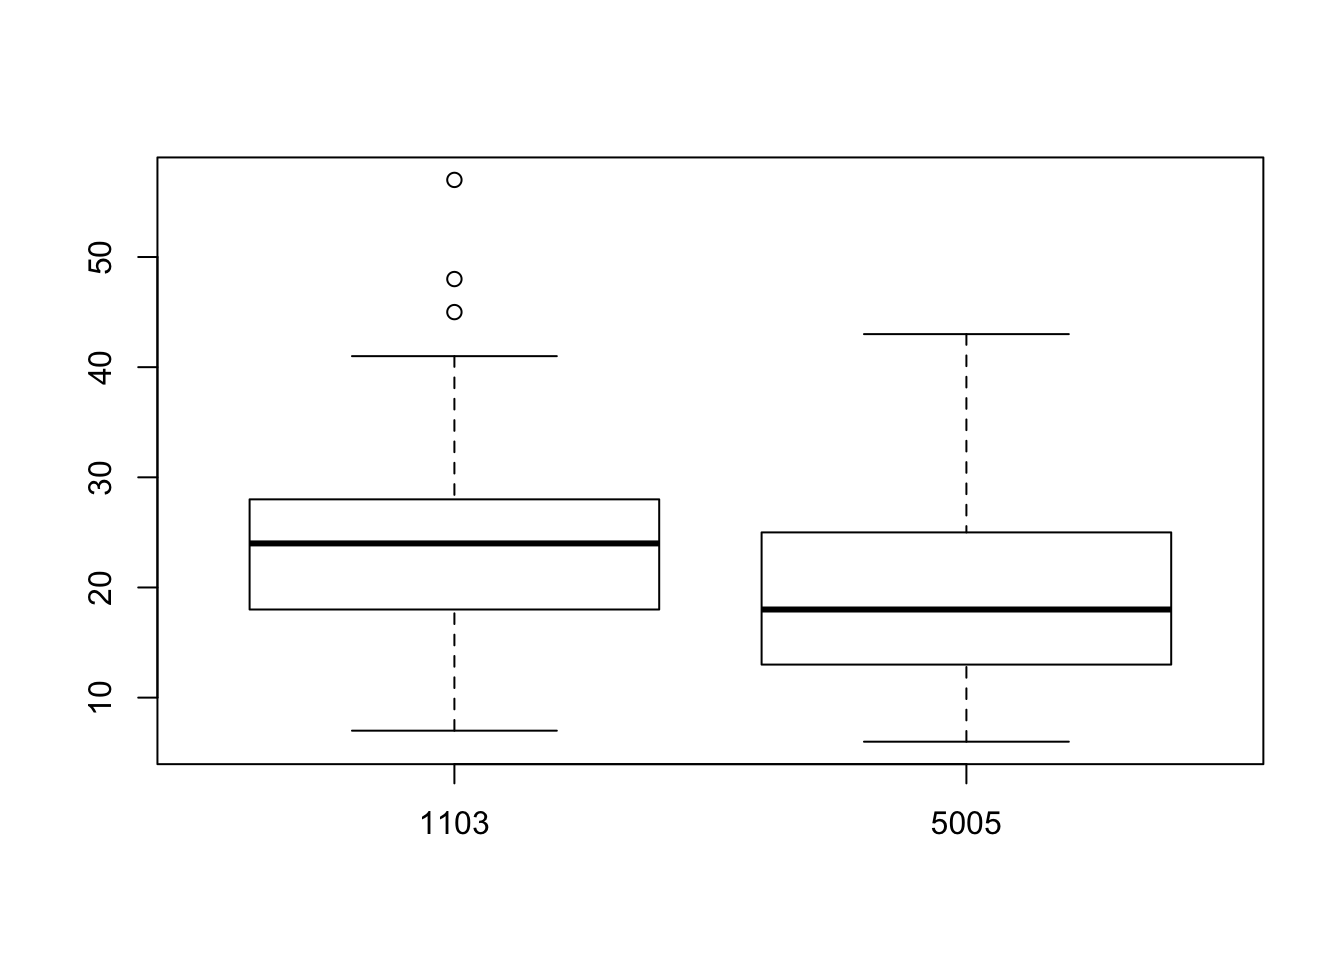
\includegraphics{bookdown_files/figure-latex/unnamed-chunk-94-1.pdf}

Possiamo notare che uno dei due siti presenta delle misurazioni che in generale sono più alte.

\begin{Shaded}
\begin{Highlighting}[]
\KeywordTok{plot}\NormalTok{(PM10dataLA}\OperatorTok{$}\NormalTok{Date.Local , PM10dataLA}\OperatorTok{$}\NormalTok{Arithmetic.Mean, }\DataTypeTok{col=}\NormalTok{ PM10dataLA}\OperatorTok{$}\NormalTok{Site.Num, }\DataTypeTok{xlab =} \StringTok{"2016"}\NormalTok{, }\DataTypeTok{ylab =} \StringTok{"mean PM10"}\NormalTok{)}
\KeywordTok{legend}\NormalTok{( }\StringTok{"topright"}\NormalTok{, }\DataTypeTok{legend =} \KeywordTok{c}\NormalTok{(}\StringTok{"1103"}\NormalTok{,}\StringTok{"5005"}\NormalTok{ ), }\DataTypeTok{col=} \KeywordTok{unique}\NormalTok{(PM10dataLA}\OperatorTok{$}\NormalTok{Site.Num), }\DataTypeTok{pch =} \KeywordTok{c}\NormalTok{(}\DecValTok{1}\NormalTok{,}\DecValTok{1}\NormalTok{) )}
\end{Highlighting}
\end{Shaded}

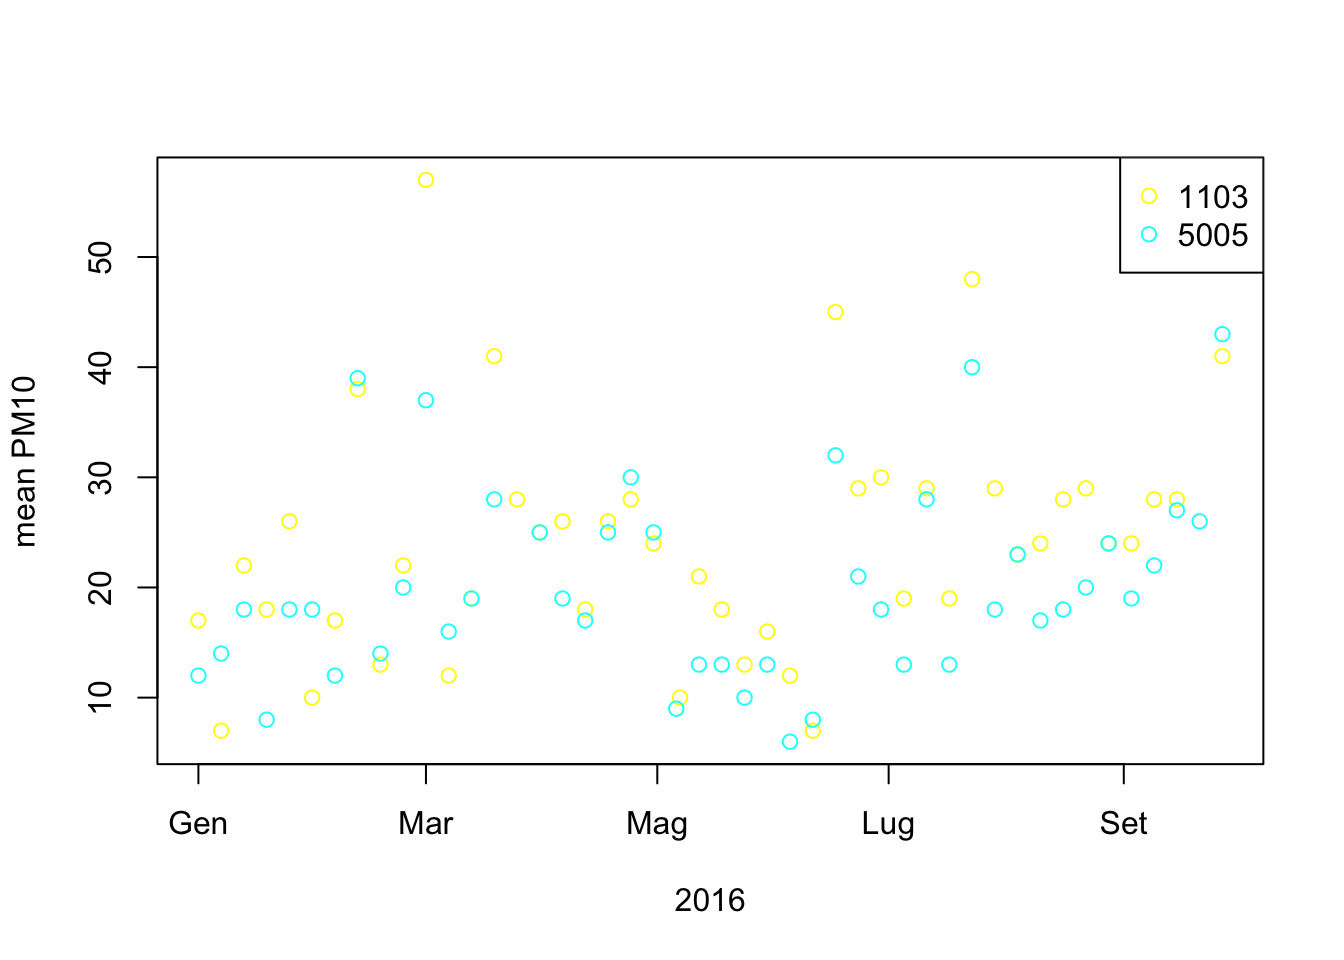
\includegraphics{bookdown_files/figure-latex/unnamed-chunk-95-1.pdf}

\hypertarget{esercizi-2}{%
\section{Esercizi}\label{esercizi-2}}

\hypertarget{esercizio-1-2}{%
\subsection{Esercizio 1}\label{esercizio-1-2}}

Si trovi un modo adeguato per importare i dati relativi al \href{http://docs.google.com/spreadsheet/pub?key=0ArfEDsV3bBwCdGhJcHAwanc2aFdZeXl1WTVZQnJjb1E\&output=xlsx}{reddito nazionale lordo pro capite} e alla \href{http://docs.google.com/spreadsheet/pub?key=0AkBd6lyS3EmpdDBKd2V5VmxkYlJuUHAtOURzUkZzNEE\&output=csv}{percentuale di strade asfaltate} in R. Dopo aver analizzato e preparato i dataset, si usino i dati per investigare le due variabili rispetto ad un paese del G7, un paese in via di sviluppo ed un paese del terzo mondo a scelta, nel periodo dal 1990 al 2009.
Si analizzino i dati e si visualizzino.

\hypertarget{esercizio-2-2}{%
\subsection{Esercizio 2}\label{esercizio-2-2}}

Si svolga il primo capitolo del \href{https://www.datacamp.com/courses/introduction-to-credit-risk-modeling-in-r}{corso online} di DataCamp che riguarda i modelli di rischio nel credito. Il primo capitolo del corso (in inglese) è gratuito.

\hypertarget{esercizio-3-1}{%
\subsection{Esercizio 3}\label{esercizio-3-1}}

Si importi il \href{https://raw.githubusercontent.com/socviz/soc880/master/data/gapminder.csv}{dataset} contenente i dati relativi alla aspettativa di vita, popolazione e prodotto interno lordo pro capite di 142 paesi del mondo.
Si aggreghino i dati per continenti e si visualizzi l'andamento dell'aspettativa di vita rispetto alle variabili tempo, reddito pro capite e popolazione.
Si investighi una possibile trasformazione dei dati per rendere più informativa l'analisi e si ripetano le analisi sui dati trasformati.

\hypertarget{esercizio-4-1}{%
\subsection{Esercizio 4}\label{esercizio-4-1}}

Si consideri il \href{https://www.kaggle.com/ronitf/heart-disease-uci}{dataset} che riporta 14 parametri di 303 pazienti con problemi di cuore. Si importi il dataset e si visualizzino con degli istogrammi le distribuzioni delle variabili. Inoltre usando la funzione \texttt{aggregate}, si determini al variare dell'età, il valore medio e massimo delle variabili \texttt{chol} (colesterolo) e \texttt{thalach} (frequenza cardiaca massima).

\hypertarget{esercizio-5}{%
\subsection{Esercizio 5}\label{esercizio-5}}

Dopo aver svolto l'Esercizio 4 del capitolo 4, si consulti il notebook R al \href{https://www.kaggle.com/naik170106027/prediction-of-heart-diseases}{link}. Quali sono gli obbiettivi dell'autore? Quale tecniche utilizza? Quale di queste non sono ancora state trattate nel nostro corso?

\hypertarget{regressione}{%
\chapter{Regressione}\label{regressione}}

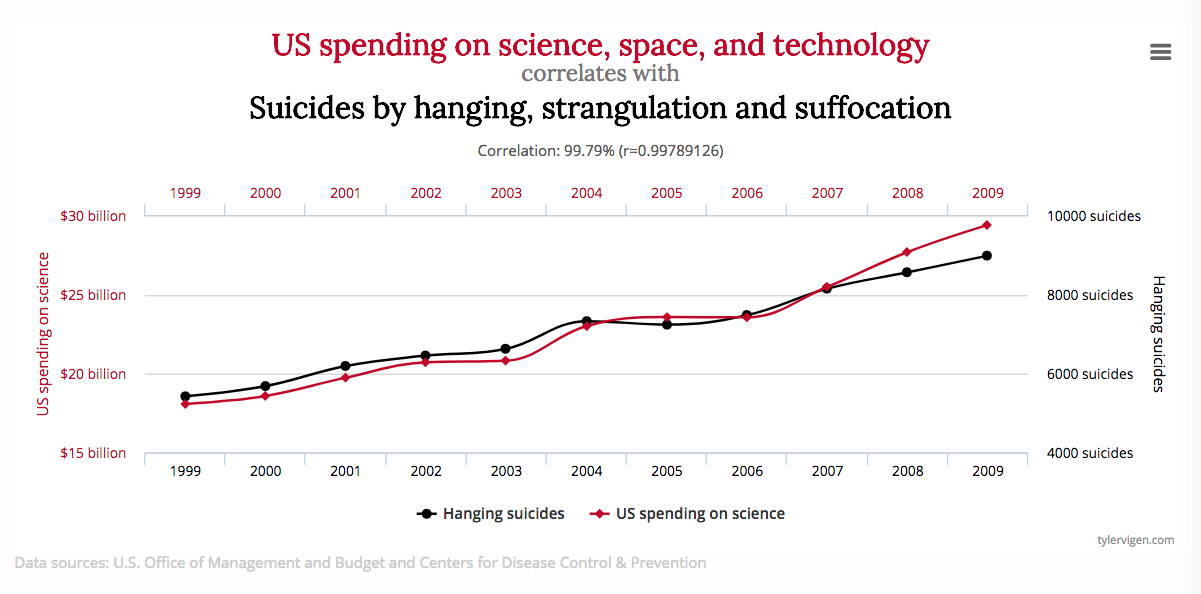
\includegraphics{./media/spurCorr.png}
Originally posted \href{http://www.tylervigen.com/spurious-correlations}{here}.

Il contenuto di questo capitolo si basa sull'omonimo capitolo del libro Calcolo delle probabilità e statistica di Paolo Baldi \citep{Baldi1998}.

Si consideri il problema, piuttosto comune, di voler esprimere una variabile, ad esempio \(y\), in funzione di altre variabili, ad esempio \(x_1, \dots , x_n\), più delle perturbazioni aleatorie.

\hypertarget{regressione-lineare}{%
\section{Regressione lineare}\label{regressione-lineare}}

Prendiamo in considerazione il caso in cui tale funzione sia lineare. Parleremo di \emph{regressione lineare}. Ciò significa che assumiamo che la variabile \(y\), detta \emph{dipendente}, si possa esprimere come
\[
y = \beta_0 + \beta_1 \cdot x + \omega
\]
dove \(\beta_0, \beta_1\) sono parametri da determinare e \(\omega\) è una perturbazione stocastica con distribuzione normale di media 0 e varianza \(\sigma^2\). I parametri \(\beta_0, \beta_1\) vengono solitamente determinati in base a diversi valori di \(x\) e \(y\).

Se abbiamo più osservazioni per la variabile \(y\), ottenute rispetto a diversi valori di \(x\), indicheremo con \(y_i\) e \(x_i\) tali valori.

Se l'assunzione che la dipendenza sia lineare è plausibile, ci aspettiamo che per le varie osservazioni valga:
\[
y_i = \beta_0 + \beta_1 x_i + \omega_i, \quad i= 1, \dots , n
\]
con \(\omega_i\) indipendenti e tutti con distribuzione \(N(0,\sigma^2)\), con \(\sigma^2\) che non dipende da \(i\).

\hypertarget{stimare-beta_0-e-beta_1}{%
\section{\texorpdfstring{Stimare \(\beta_0\) e \(\beta_1\)}{Stimare \textbackslash{}beta\_0 e \textbackslash{}beta\_1}}\label{stimare-beta_0-e-beta_1}}

Il problema di stimare \(\beta_0, \beta_1\) viene risolto andando a trovare quei valori per i parametri che minimizzano la distanza tra i dati osservati (\(y_i\)) e i valori prodotti dal modello:
\[
\hat{y_i} = \beta_0 + \beta_1 x_i
\]
La formulazione diviene quindi:
\[
\min_{\beta_0, \beta_1 } S = S(\beta_0, \beta_1 ) = \sum_{i=1}^n \left( y_i - \beta_0 + \beta_1 x_i \right)^2
\]

Questo problema di minimizzazione quadratica ammette soluzione (unica) e si può ottenere andando ad imporre che il gradiente si annulli. Questo porta alla soluzione \((b_0, b_1)\) tale che:
\[
b_0  = \bar{y} - b_1 \bar{x}
\]

\[
b_1 = \frac{\sum_i (y_i - \bar{y}) x_i}{\sum_i x_i (x_i - \bar{x})} = \frac{\bar{\sigma}
_{x y }} {\bar{\sigma_{x}^2}}
\]
con
\[
 \bar{x} = \frac{1}{n} \sum_i x_i \, \text{ e } \bar{y} = \frac{1}{n} \sum_i y_i
\]
I valori di \(b_0\) e \(b_1\) così ottenuti sono \emph{stimatori} per i parametri \(\beta_0\) e \(\beta_1\). In particolare è possibile dimostrare che sono degli stimatori \textbf{non distorti}.

Inoltre c'è tutta una serie di risultati (che non dimostreremo) che permettono di provare, usando anche le ipotesi sugli \(\omega_i\), che:
\[
b_0 \sim N\left( \beta_0, \sigma^2 (\frac{1}{n} + \frac{\bar{x}^2}{\bar{\sigma}_x^2}) \right), \, b_1 \sim N\left( \beta_1, \frac{\sigma^2}{\bar{\sigma}_x^2}) \right)
\]
Ovviamente è possibile associare degli intervalli di confidenza ai valori ottenuti, così come eseguire altri test statistici, ma noi non tratteremo questa parte.

Se indichiamo con \(r_i = y_i - \hat{y_i}\), i così detti \textbf{residui}, possiamo definire:
\[
s^2 = \frac{1}{n-2} \sum_i r_i^2 
\]
che è uno stimatore non distorto di \(\sigma^2\), la varianza (sconosciuta) delle perturbazioni aleatorie. Inoltre vale che:
\[
\frac{s^2}{\sigma^2}(n-2) \sim \chi^2(n-2)
\]
dove \(\chi^2\) indica la distribuzione \href{https://it.wikipedia.org/wiki/Distribuzione_chi_quadrato}{Chi quadrato}.
Usando R con il comando \texttt{lm()} è possibile non solo definire un modello di regressione lineare, ma anche accedere a molte di queste informazioni.

\hypertarget{valutare-il-modello-r2}{%
\section{\texorpdfstring{Valutare il modello: \(R^2\)}{Valutare il modello: R\^{}2}}\label{valutare-il-modello-r2}}

Un utile valore per valutare la correttezza del modello, è il valore di \(R^2\), definito come:
\[
R^2 = \frac{\sum_i (\hat{y_i} - \bar{y} )^2}{\sum_i (y_i - \bar{y})^2} = 1 -\frac{\sum_i (y_i - \hat{y_i})^2}{\sum_i (y_i - \bar{y})^2} 
\]

Questo valore, che assume valori tra 0 e 1, quantifica la proporzione di varianza dei dati che è spiegata dal modello. Più tale valore si avvicina a 1, migliore è il modello. Se invece tale valore è piccolo, o il modello è inadeguato (relazione non lineare o ipotesi non soddisfatte), o \(\sigma^2\) potrebbe avere un valore elevato.

\hypertarget{regressione-lineare-in-r}{%
\section{Regressione lineare in R}\label{regressione-lineare-in-r}}

Ricordiamo che per applicare la regressione lineare dobbiamo essere sicuri che le ipotesi siano soddisfatte. In particolare dovremo assicurarci che i residui seguano una distribuzione normale centrata in 0 e siano indipendenti.

Alcune delle funzioni già viste possono aiutarci in questo compito.

Definire e richiamare un modello lineare in R è molto semplice. Basta infatti utilizzare la funzione \texttt{lm()}, dove va specificata la \emph{variabile dipendente} e il \emph{predittore} ed i dati da usare per definire il modello.

Sebbene i modelli di \emph{regressione multipla} siano concettualmente e praticamente più complessi, R li supporta usando la stessa funzione e la stessa notazione. In tal caso, invece che indicare un predittore, se ne indicano più usando il simbolo \texttt{+} per elencarli.

\hypertarget{mtcars}{%
\subsection{Mtcars}\label{mtcars}}

Vediamo alcuni esempi usando il dataset \texttt{mtcars}.

Supponiamo di voler investigare se il consumo di carburante e il numero di cavalli seguono una relazione lineare.

Un ottimo metodo per intuire se la relazione possa essere in qualche modo lineare è quello di disegnare la variabile dipendente in funzione del predittore.

\begin{Shaded}
\begin{Highlighting}[]
\KeywordTok{plot}\NormalTok{(mpg }\OperatorTok{~}\StringTok{ }\NormalTok{hp, }\DataTypeTok{data =}\NormalTok{ mtcars)}
\end{Highlighting}
\end{Shaded}

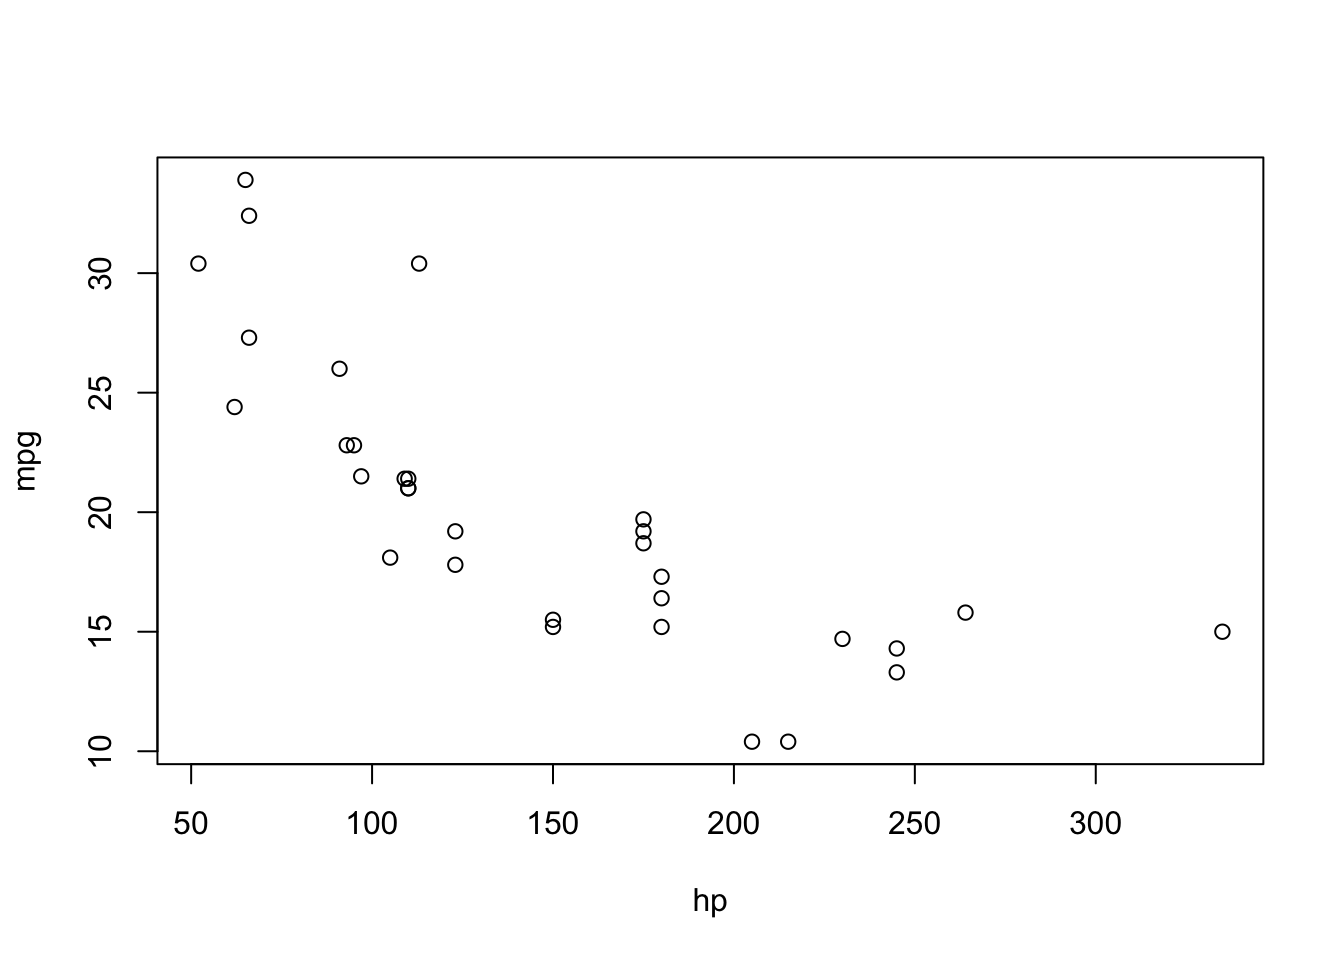
\includegraphics{bookdown_files/figure-latex/unnamed-chunk-96-1.pdf}

Secondo i risultati della nostra analisi preliminare sembra plausibile che la relazione sia lineare. Continuiamo la nostra investigazione definendo il modello con la funzione \texttt{lm()} e visualizzando il risultato usando la ben nota funzione \texttt{summary()}.

\begin{Shaded}
\begin{Highlighting}[]
\NormalTok{mtcars_reg <-}\StringTok{ }\KeywordTok{lm}\NormalTok{(mpg }\OperatorTok{~}\StringTok{ }\NormalTok{hp, }\DataTypeTok{data =}\NormalTok{ mtcars)}
\KeywordTok{summary}\NormalTok{(mtcars_reg)}
\end{Highlighting}
\end{Shaded}

\begin{verbatim}
## 
## Call:
## lm(formula = mpg ~ hp, data = mtcars)
## 
## Residuals:
##     Min      1Q  Median      3Q     Max 
## -5.7121 -2.1122 -0.8854  1.5819  8.2360 
## 
## Coefficients:
##             Estimate Std. Error t value Pr(>|t|)    
## (Intercept) 30.09886    1.63392  18.421  < 2e-16 ***
## hp          -0.06823    0.01012  -6.742 1.79e-07 ***
## ---
## Signif. codes:  0 '***' 0.001 '**' 0.01 '*' 0.05 '.' 0.1 ' ' 1
## 
## Residual standard error: 3.863 on 30 degrees of freedom
## Multiple R-squared:  0.6024, Adjusted R-squared:  0.5892 
## F-statistic: 45.46 on 1 and 30 DF,  p-value: 1.788e-07
\end{verbatim}

Si può accedere ai vari elementi elencati da \texttt{summary()} usando la notazione \texttt{\$}.

Tra le informazioni che fornisce summary, è presente anche il valore \textbf{R-squared} (R quadro), che è la \textbf{proporzione di varianza della variabile dipendente che viene spiegata dal predittore}. Tale valore è compreso tra 0 e 1. Valori vicino a 1 indicano un buon modello, mentre valori bassi possono indicare o che il modello non spieghi completamente/correttamente i dati, o che la varianza dei residui è molto alta.

Una volta definito il modello, è importante visualizzare i risultati per valutarne la bontà e per capire il comportamento dei residui. In questo modo è infatti possibile verificare \textbf{quantitativamente} (non formalmente) se i residui soddisfano le ipotesi di indipendenza (non si devono osservare dei pattern) e che la distribuzione dei quantili sia confrontabile con quella di una normale.

I seguenti comandi permettono di visualizzare la retta di regressione, i quantili e di confrontarli con la distribuzione in quantili di una normale.

\begin{Shaded}
\begin{Highlighting}[]
\KeywordTok{par}\NormalTok{(}\DataTypeTok{mfrow =} \KeywordTok{c}\NormalTok{(}\DecValTok{3}\NormalTok{,}\DecValTok{1}\NormalTok{), }\DataTypeTok{mar =} \KeywordTok{c}\NormalTok{(}\DecValTok{2}\NormalTok{,}\DecValTok{2}\NormalTok{,}\DecValTok{1}\NormalTok{,}\DecValTok{1}\NormalTok{))}
\CommentTok{# Retta di regressione}
\KeywordTok{plot}\NormalTok{(mpg }\OperatorTok{~}\StringTok{ }\NormalTok{hp, }\DataTypeTok{data =}\NormalTok{ mtcars)}
\KeywordTok{abline}\NormalTok{(mtcars_reg}\OperatorTok{$}\NormalTok{coefficients, }\DataTypeTok{col =} \StringTok{"red"}\NormalTok{)}
\CommentTok{# Pattern nei residui}
\KeywordTok{plot}\NormalTok{(mtcars_reg}\OperatorTok{$}\NormalTok{residuals, }\DataTypeTok{main =} \StringTok{"Residui"}\NormalTok{)}
\CommentTok{# Distribuzione in quantili }
\KeywordTok{qqnorm}\NormalTok{(mtcars_reg}\OperatorTok{$}\NormalTok{residuals)}
\KeywordTok{qqline}\NormalTok{(mtcars_reg}\OperatorTok{$}\NormalTok{residuals)}
\end{Highlighting}
\end{Shaded}

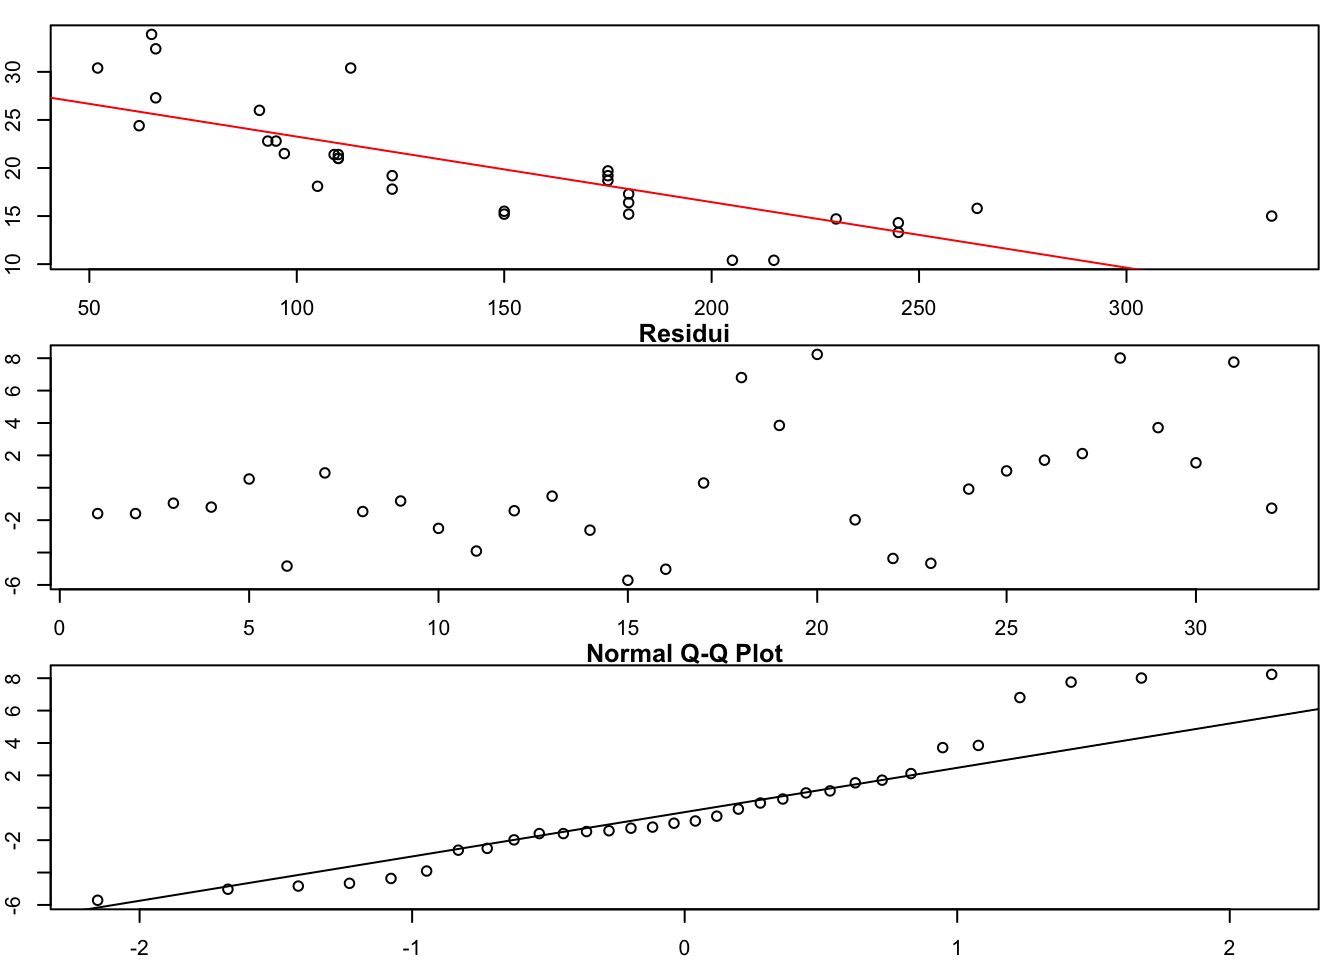
\includegraphics{bookdown_files/figure-latex/unnamed-chunk-98-1.pdf}

\hypertarget{esercizio-a}{%
\subsubsection*{Esercizio A}\label{esercizio-a}}
\addcontentsline{toc}{subsubsection}{Esercizio A}

In modo analogo a quanto fato sopra, si investighi la relazione tra consumo e peso delle auto in esame.

\hypertarget{esercizio-b}{%
\subsubsection*{Esercizio B}\label{esercizio-b}}
\addcontentsline{toc}{subsubsection}{Esercizio B}

Si discuta un modello lineare per le variabili \textbf{x} e \textbf{y} di \textbf{Esercizo 1}.

\hypertarget{regressione-multipla}{%
\section{Regressione multipla}\label{regressione-multipla}}

Come anticipato, se volessimo considerare una regressione multipla, e per esempio considerare come predittori sia la potenza (cavalli) che il peso, possiamo implementare il modello in modo simile in R.

\begin{Shaded}
\begin{Highlighting}[]
\NormalTok{mtcars_reg_hp_wt <-}\StringTok{ }\KeywordTok{lm}\NormalTok{(mpg }\OperatorTok{~}\StringTok{ }\NormalTok{hp }\OperatorTok{+}\StringTok{ }\NormalTok{wt, }\DataTypeTok{data =}\NormalTok{ mtcars)}
\KeywordTok{summary}\NormalTok{(mtcars_reg_hp_wt)}
\end{Highlighting}
\end{Shaded}

\begin{verbatim}
## 
## Call:
## lm(formula = mpg ~ hp + wt, data = mtcars)
## 
## Residuals:
##    Min     1Q Median     3Q    Max 
## -3.941 -1.600 -0.182  1.050  5.854 
## 
## Coefficients:
##             Estimate Std. Error t value Pr(>|t|)    
## (Intercept) 37.22727    1.59879  23.285  < 2e-16 ***
## hp          -0.03177    0.00903  -3.519  0.00145 ** 
## wt          -3.87783    0.63273  -6.129 1.12e-06 ***
## ---
## Signif. codes:  0 '***' 0.001 '**' 0.01 '*' 0.05 '.' 0.1 ' ' 1
## 
## Residual standard error: 2.593 on 29 degrees of freedom
## Multiple R-squared:  0.8268, Adjusted R-squared:  0.8148 
## F-statistic: 69.21 on 2 and 29 DF,  p-value: 9.109e-12
\end{verbatim}

\hypertarget{esercitazione-1}{%
\chapter{Esercitazione 1}\label{esercitazione-1}}

Si scarichi il dataset al \href{https://www.dropbox.com/s/8uoacrlaeio1hy3/DataL5.tsv?dl=1}{link} e si eseguano le operazioni:

\begin{enumerate}
\def\labelenumi{\arabic{enumi}.}
\tightlist
\item
  Si importi il dataset.
\item
  Si crei un nuovo dataset contenente solo le righe corrispondenti alla variabile \textbf{Idataset} uguale all'ultimo numero del proprio numero di matricola. Dopo aver fatto ciò, si rimuova la variabile. Le seguenti analisi si intendono su questo dataset.
\item
  Si analizzi la struttura del dataset, si verifichi il numero di righe e colonne contenute. Il dataset è stato letto bene? E' tidy?
\item
  Si verifichi la presenza di eventuali errori nei dati e si sostituiscano con la mediana.
\item
  Si calcolino media, mediana, minimo, massimo e quartili e deviazione standard.
\item
  Si visualizzi la distribuzione delle variabili \textbf{x} e \textbf{y} e i loro box plot.
\item
  Si visualizzino i dati mediante uno scatterplot.
\end{enumerate}

Il dataset completo e una discussione riguardo i dati usati per l'esercizio sono disponibili \href{https://www.autodeskresearch.com/publications/samestats}{qui}.

\hypertarget{esercizi-3}{%
\section{Esercizi}\label{esercizi-3}}

\hypertarget{esercizio-1-3}{%
\subsection{Esercizio 1}\label{esercizio-1-3}}

Si importi il \href{https://www.dropbox.com/s/boesoonvh04nqym/Gray_Kangaroos.tsv?dl=1}{dataset} (\href{http://college.cengage.com/mathematics/brase/understandable_statistics/7e/students/datasets/slr/frames/frame.html}{descrizione}) e si analizzi la relazione tra le due variabili usando la regressione lineare. Si analizzino i risultati e si visualizzino i residui.

\hypertarget{esercizio-2-3}{%
\subsection{Esercizio 2}\label{esercizio-2-3}}

Si trovi un modo adeguato per importare i dati relativi al \href{http://docs.google.com/spreadsheet/pub?key=0ArfEDsV3bBwCdGhJcHAwanc2aFdZeXl1WTVZQnJjb1E\&output=xlsx}{reddito nazionale lordo pro capite} e alla \href{http://docs.google.com/spreadsheet/pub?key=0AkBd6lyS3EmpdDBKd2V5VmxkYlJuUHAtOURzUkZzNEE\&output=csv}{percentuale di strade asfaltate} in R. Dopo aver analizzato e preparato i dataset, si usino i dati per investigare le due variabili rispetto ad un paese del G7, un paese in via di sviluppo ed un paese del terzo mondo a scelta, nel periodo dal 1990 al 2009.
Si analizzino i dati e si visualizzino. Inoltre si usi la regressione lineare per analizzare la relazione tra le variabili. Si commentino e discutano i risultati.

\hypertarget{esercizio-3-2}{%
\subsection{Esercizio 3}\label{esercizio-3-2}}

Usando il dataset ottenuto nell'Esercizio 3 del capitolo 5, si investighi usando la regressione lineare la relazione tra prodotto interno lordo e aspettativa di vita per ognuno dei continenti. Si usi la funzione \texttt{predict()} per valutare il modello su dati diversi da quelli usati per definirlo. In particolare, si valuti il modello ottenuto per l'America sui dati europei e viceversa. Si visualizzino e si discutano i risultati ottenuti, dandone anche un interpretazione.

\hypertarget{esercizio-4-2}{%
\subsection{Esercizio 4}\label{esercizio-4-2}}

Si considerino i modelli ottenuto nell'Esercizio 3. Si valuti separatamente il modello ottenuto per l'America e quello l'Europa usando i dati dei paesi \emph{Canada}, \emph{Italy}, \emph{Argentina} e \emph{Sierra Leone} contentuti nel dataset originale. Si valutino i valori di R quadro ottenuti e si discutano i risultati.

\emph{Suggerimento} si usi la formulazione equivalente di R quadro:

\bibliography{book.bib,packages.bib}


\end{document}
